\documentclass[11pt]{article}

\usepackage[a4paper,margin=2.2cm]{geometry}
\usepackage{amsmath}
\usepackage{booktabs}
\usepackage{caption}
\usepackage{float}
\usepackage{graphicx}
\usepackage{hyperref}
\usepackage{listings}
\usepackage{placeins}
\usepackage{subcaption}
\usepackage{xcolor}

\graphicspath{{../outputs/figures_en/}}
\hypersetup{colorlinks=true, linkcolor=blue, urlcolor=blue}
\setlength{\parindent}{0pt}
\setlength{\parskip}{0.45em}
\captionsetup{font=small, labelfont=bf}
\lstset{
  basicstyle=\ttfamily\small,
  breaklines=true,
  frame=single,
  columns=fullflexible,
  keepspaces=true,
  keywordstyle=\color{blue!60!black},
  commentstyle=\color{green!35!black}
}

\title{\textbf{Experiment 2: Spectral Estimation Lab Report}}
\author{Yanzhe Zhao}
\date{April 30, 2026}

\begin{document}
\maketitle

\begin{abstract}
This report completes four spectral-estimation experiments on synthetic signals and closed-eye resting-state EEG from the LEMON dataset. All spectra are shown as absolute one-sided power spectral density in dB/Hz, without per-curve normalization. The experiments compare direct FFT, windowed periodogram, autocorrelation, Welch, and Yule-Walker AR spectra, with emphasis on bias-variance trade-offs, leakage, resolution, zero-padding interpretation, AR order selection, and statistical stability.
\end{abstract}

\section{Data, Methods, and Reproducibility}

\subsection{Data and Segments}
The synthetic signals use a sampling rate of 250 Hz and fixed random seed 20260430. The real EEG data are the provided LEMON EC EEGLAB \texttt{.set/.fdt} files, containing 60 channels sampled at 250 Hz. The Oz channel is used throughout. The main real EEG segment for Experiments 1 and 2 is 58.84--117.84 s, the segment for Experiment 3 is 126.61--134.61 s, and the segment for Experiment 4 is 58.84--112.84 s.

EEG samples are internally represented in volts. MNE is used first; if the legacy file name inside the EEGLAB \texttt{.set} file prevents MNE loading, the fallback reader loads the metadata with \texttt{scipy.io.loadmat}, reads the \texttt{.fdt} file with \texttt{np.fromfile}, and multiplies the microvolt-scale EEGLAB data by 0.000001. This keeps the absolute dB/Hz scale consistent between the MNE and fallback paths.

\subsection{Common PSD Convention}
For windowed FFT-based spectra, the one-sided density estimate is
\[
P_{xx}(f)=\frac{|\mathrm{FFT}\{x[n]w[n]\}|^2}{f_s\sum_n w^2[n]},
\]
with one-sided doubling for non-DC, non-Nyquist bins. The direct method is the rectangular-window full-record FFT. The periodogram method differs mainly through the window. The autocorrelation method uses the biased full-lag autocorrelation sequence followed by an FFT; under this full-lag rectangular setting it is expected to be nearly equivalent to the direct FFT by the Wiener-Khinchin relation. A truncated or additionally windowed autocorrelation sequence would produce a visibly smoother but more biased estimate.

Welch spectra average overlapping short-window periodograms. This reduces estimator variance but uses the segment length, not the full record length, as the effective resolution scale. AR spectra use Yule-Walker parameter estimation. FPE is used as an order-selection criterion:
\[
\mathrm{FPE}(p)=\hat{\sigma}_p^2\frac{N+p+1}{N-p-1}.
\]
Alpha metrics are defined in the 8--13 Hz band. Alpha prominence is the alpha peak power minus the mean 15--30 Hz background power.

\subsection{Reproduction Commands}
\begin{verbatim}
.\.venv\Scripts\python.exe -m experiments.run_all
.\.venv\Scripts\python.exe -m experiments.run_all_en
.\.venv\Scripts\python.exe report\build_report_en.py
\end{verbatim}

\begin{figure}[H]
\centering
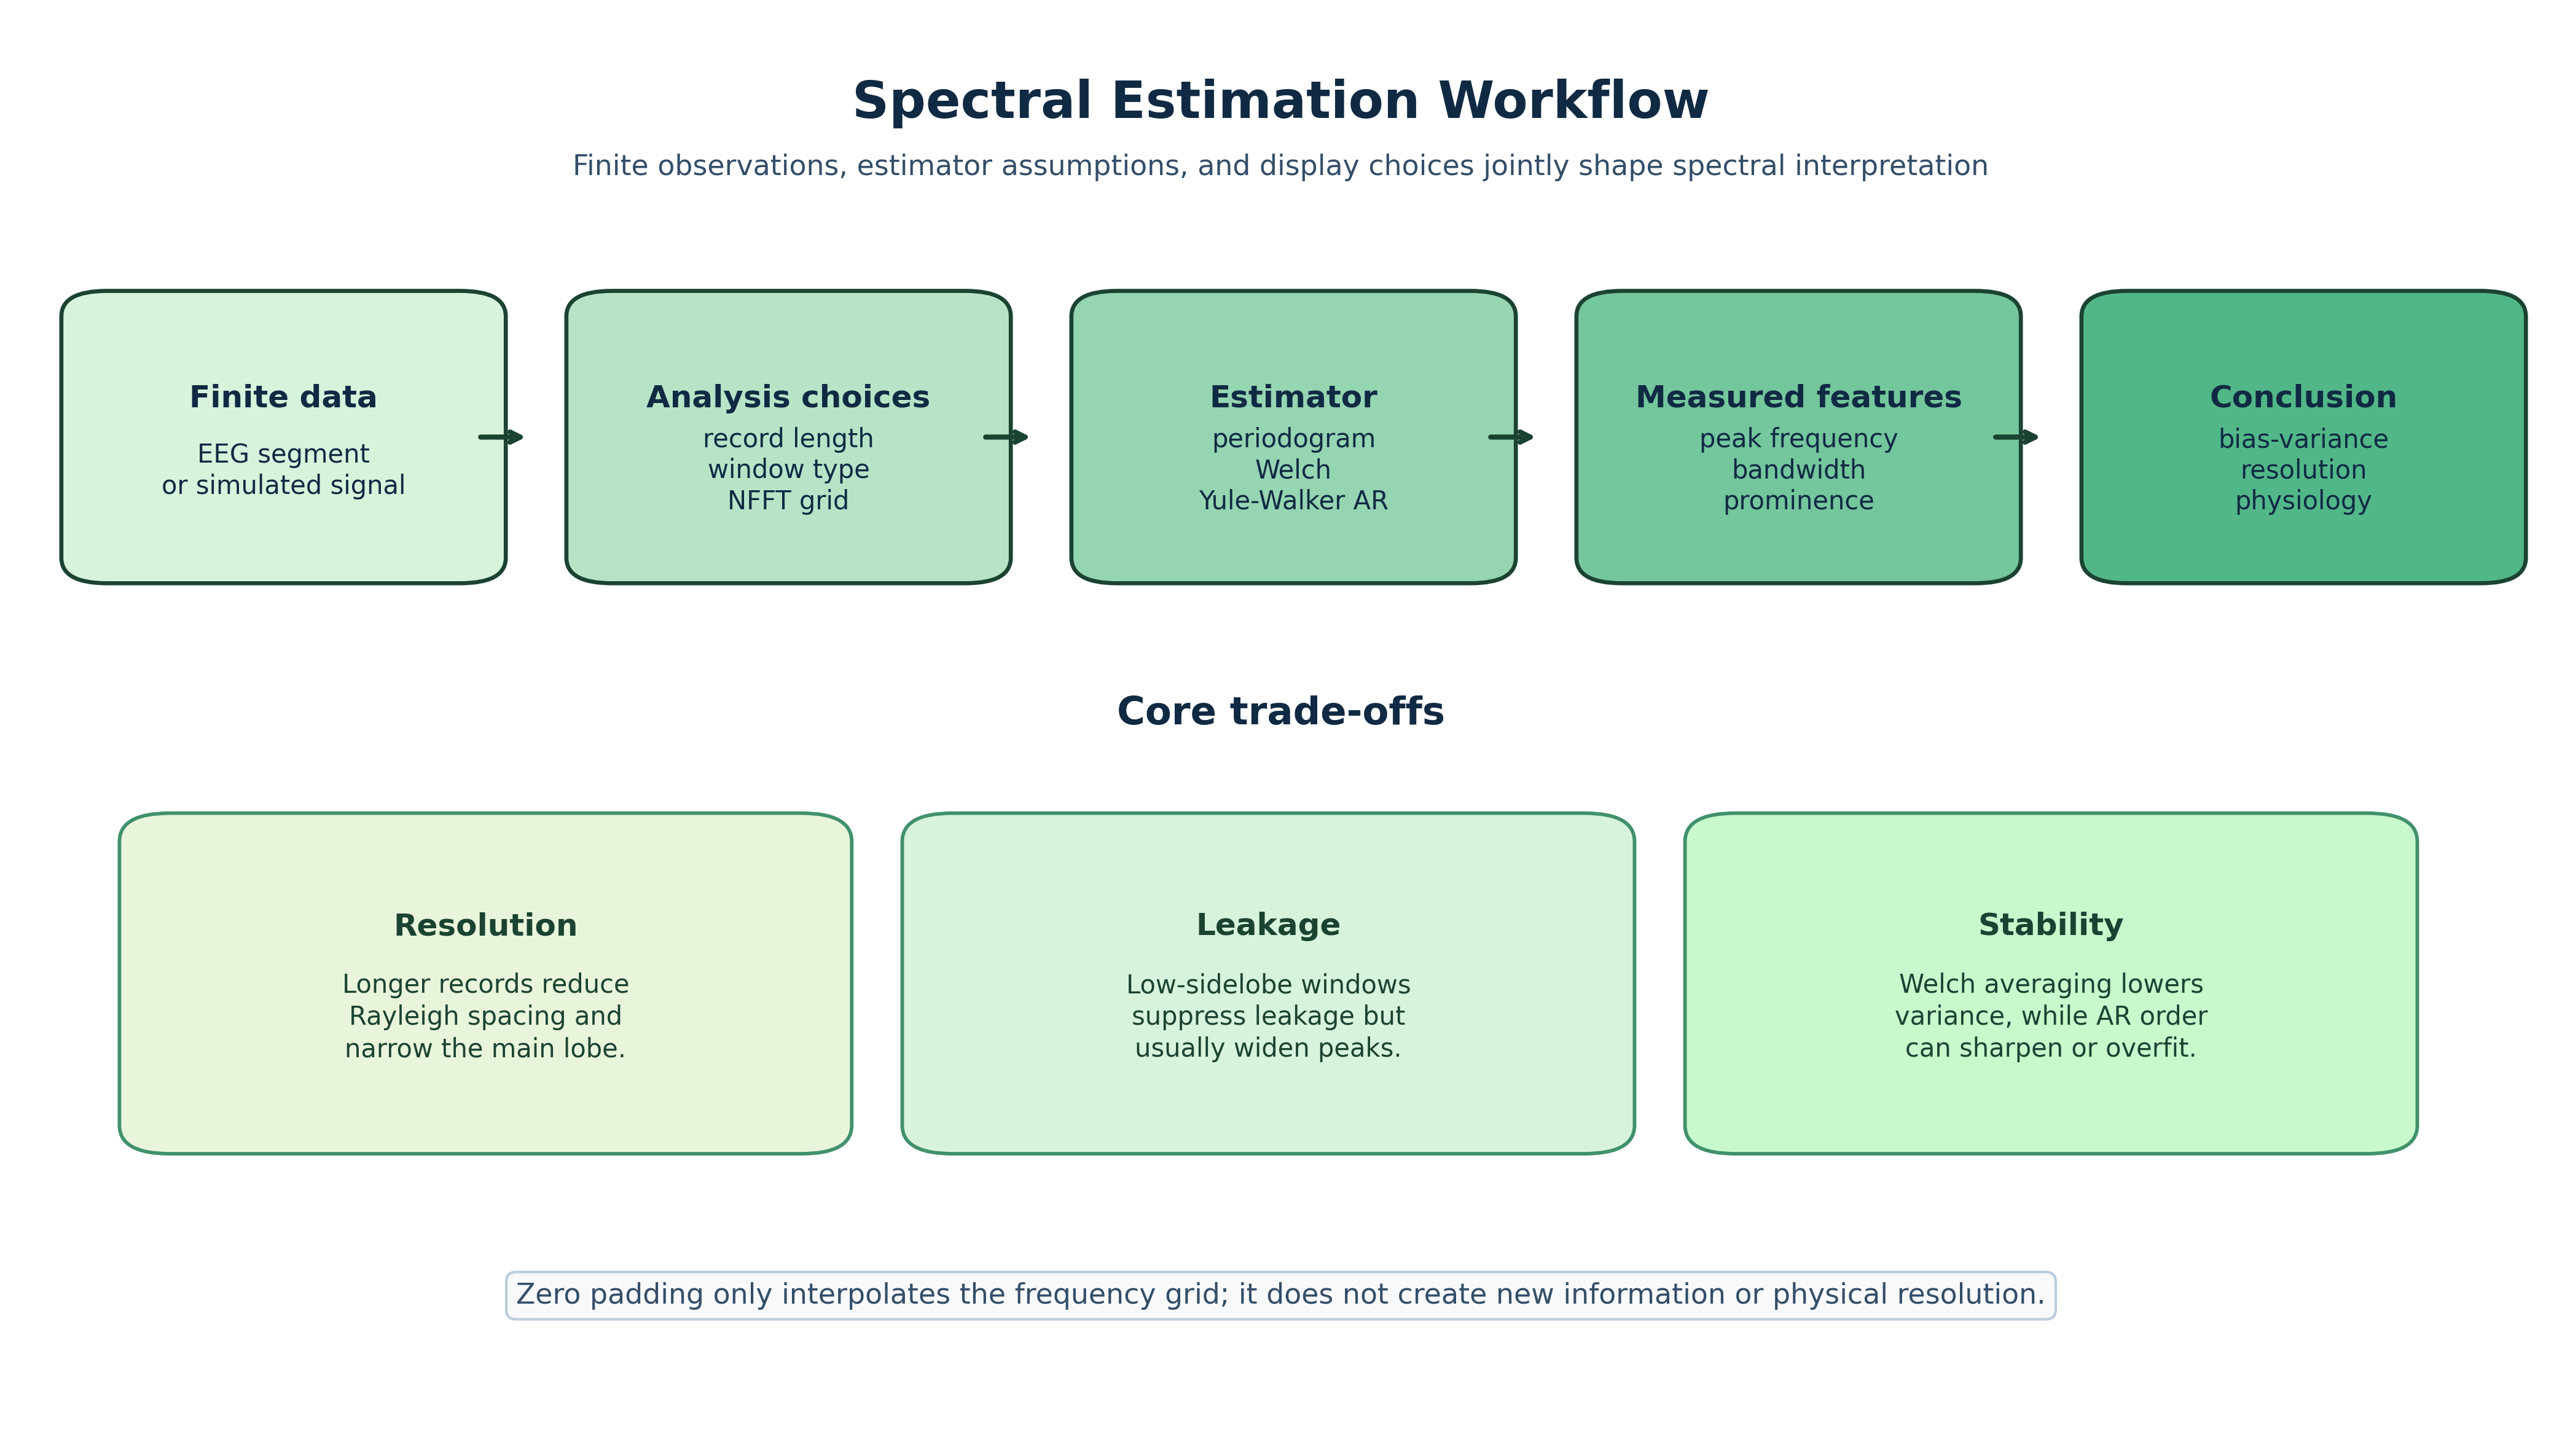
\includegraphics[width=\textwidth]{spectral_pipeline_mechanism_en.png}
\caption{Spectral estimation workflow and the core methodological trade-offs.}
\end{figure}

\section{Experiment 1: Classical Nonparametric PSD Estimates}

\subsection{Design}
The artificial signal is
\[
x(t)=\sin(2\pi\cdot12t)+0.6\sin(2\pi\cdot24t)+0.8w(t),
\]
where $w(t)$ is zero-mean unit-variance Gaussian noise. Direct FFT, Hamming periodogram, full-lag autocorrelation, and Welch spectra are compared on the same data. Welch uses 1 s segments, 50\% overlap, and a Hamming window. The same four estimators are then applied to the Oz EEG segment from 58.84 to 117.84 s.

\begin{figure}[H]
\centering
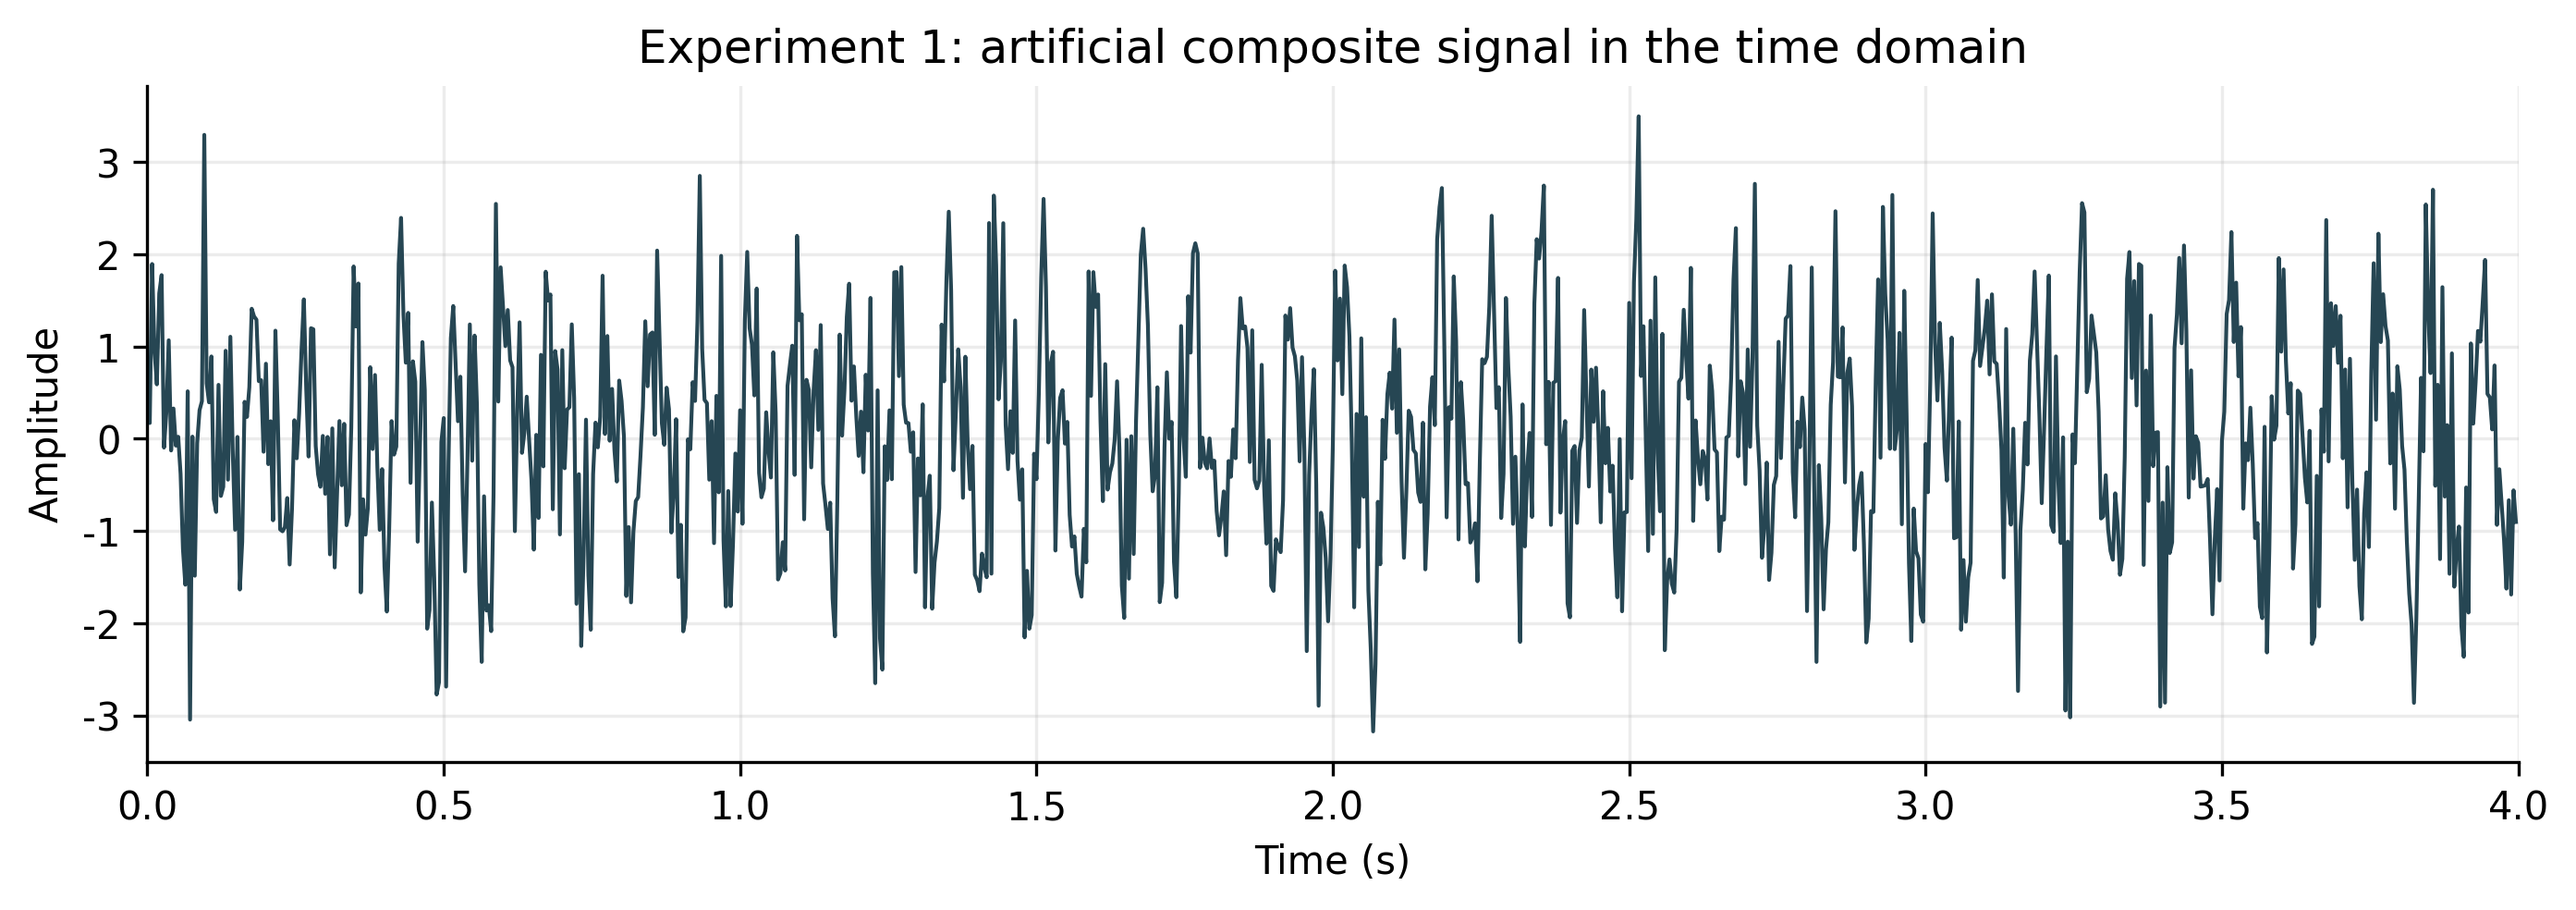
\includegraphics[width=\textwidth]{exp1_artificial_time_signal_en.png}
\caption{Time-domain artificial signal.}
\end{figure}

\begin{figure}[H]
\centering
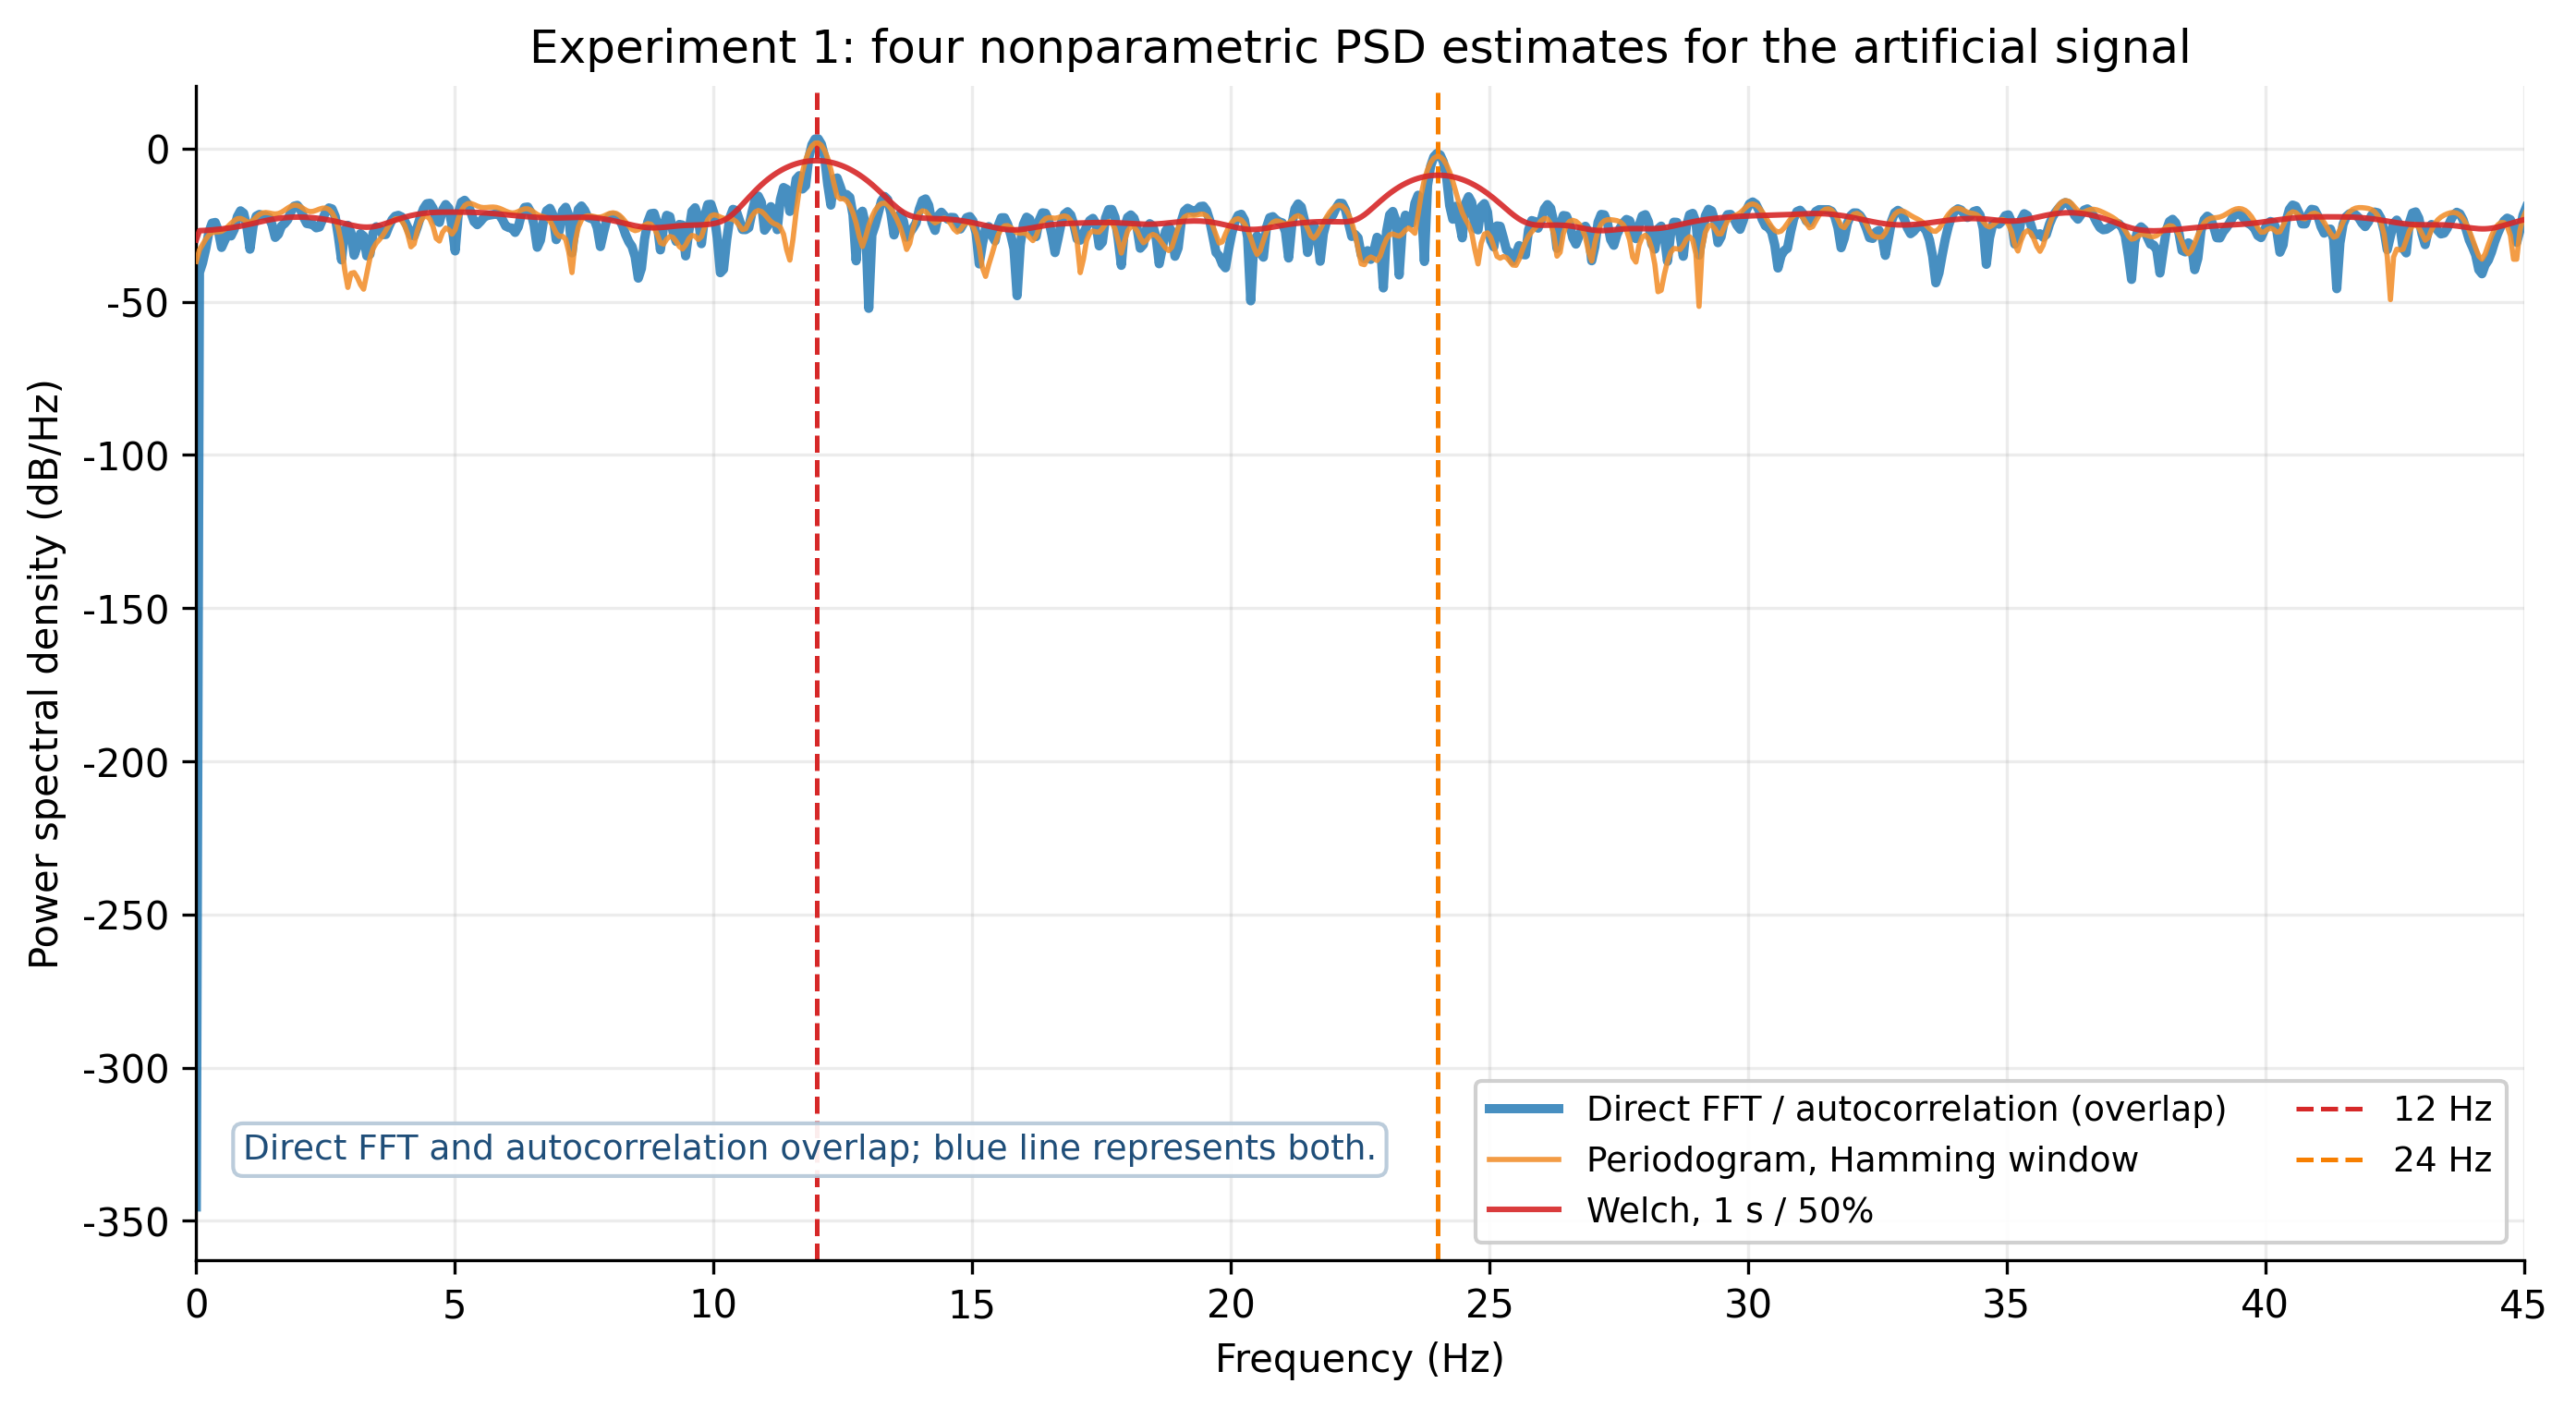
\includegraphics[width=\textwidth]{exp1_artificial_methods_en.png}
\caption{Four nonparametric PSD estimates for the artificial signal.}
\end{figure}

\input{generated_en/table_exp1_artificial.tex}

\begin{figure}[H]
\centering
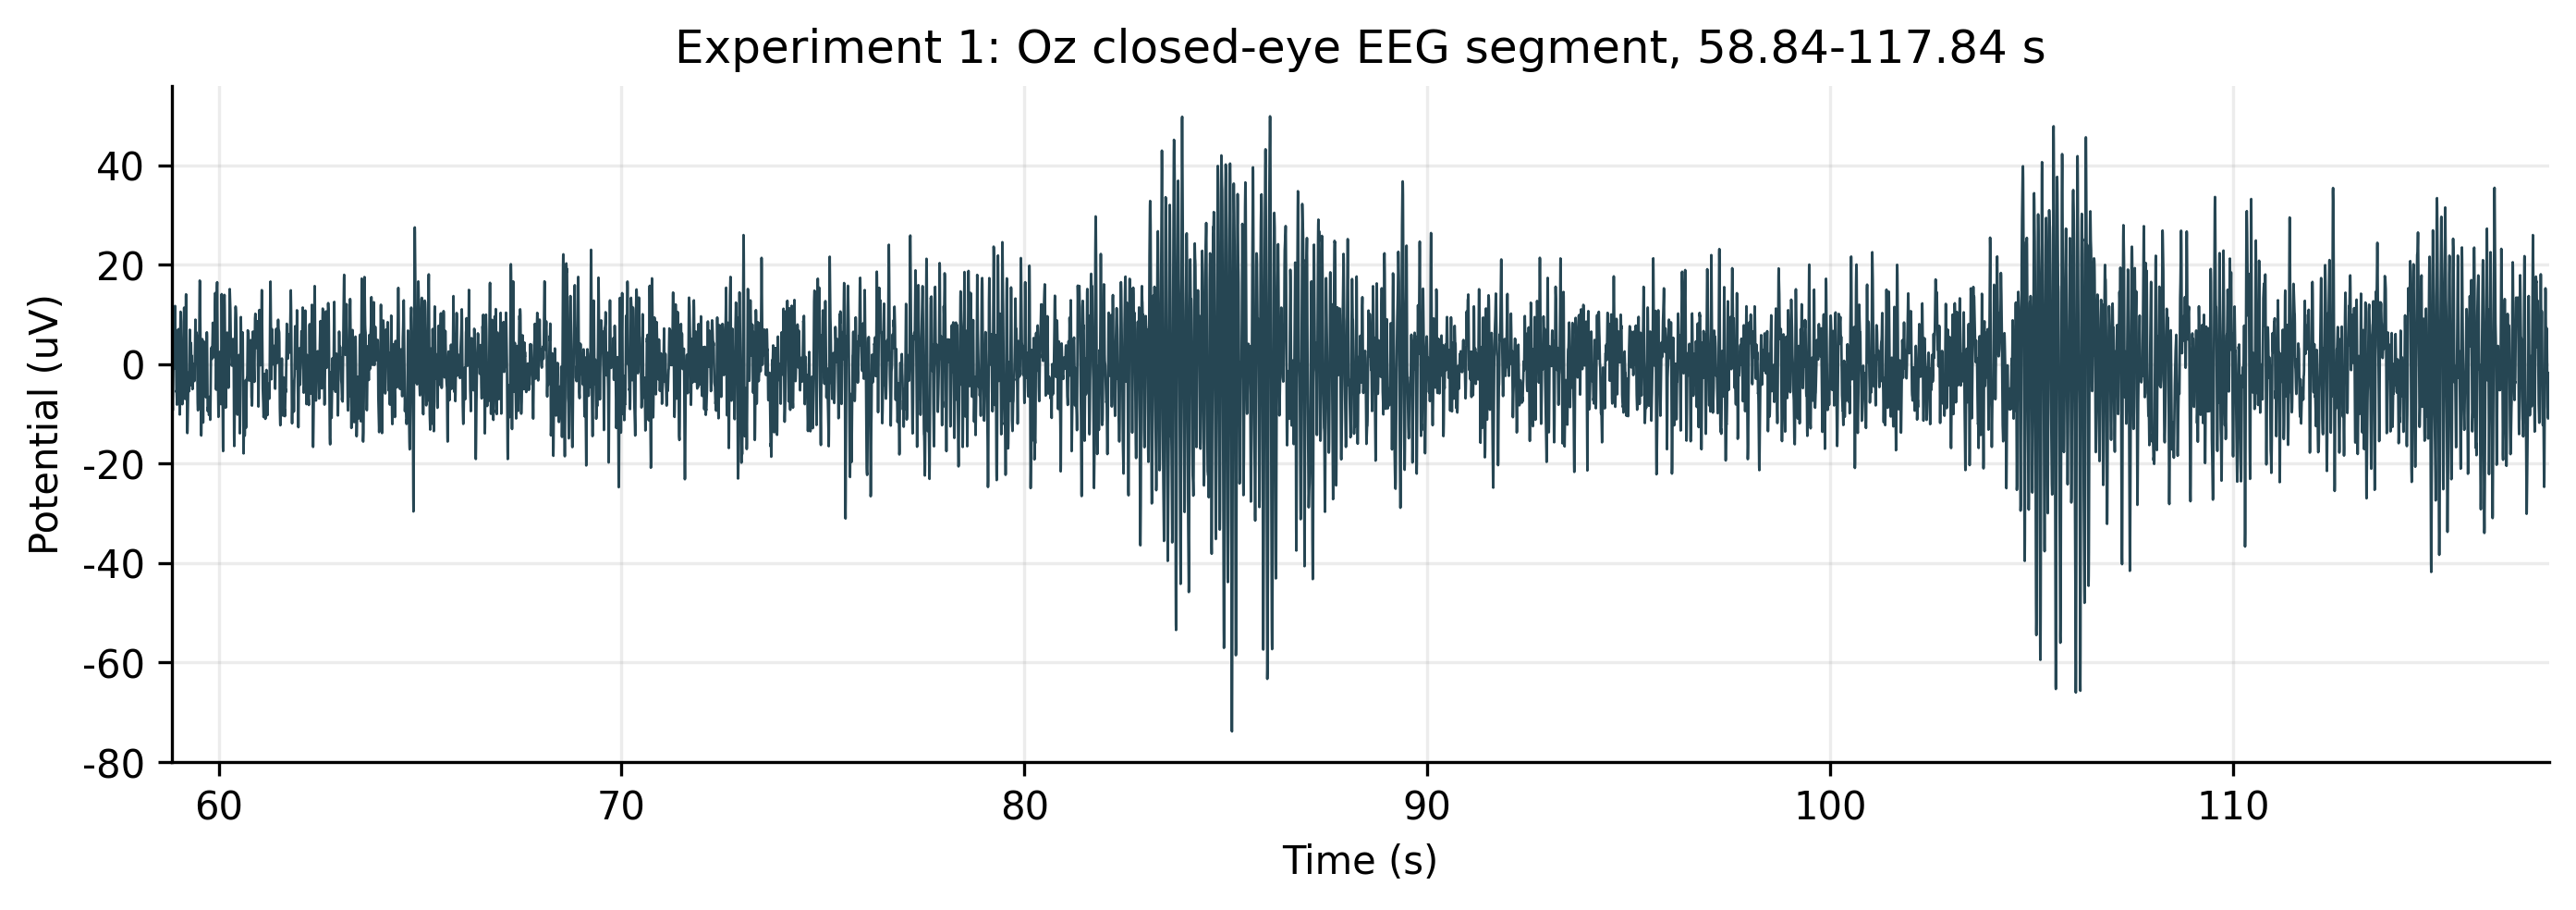
\includegraphics[width=\textwidth]{exp1_real_eeg_time_segment_en.png}
\caption{Oz closed-eye EEG segment used for the real-data comparison.}
\end{figure}

\begin{figure}[H]
\centering
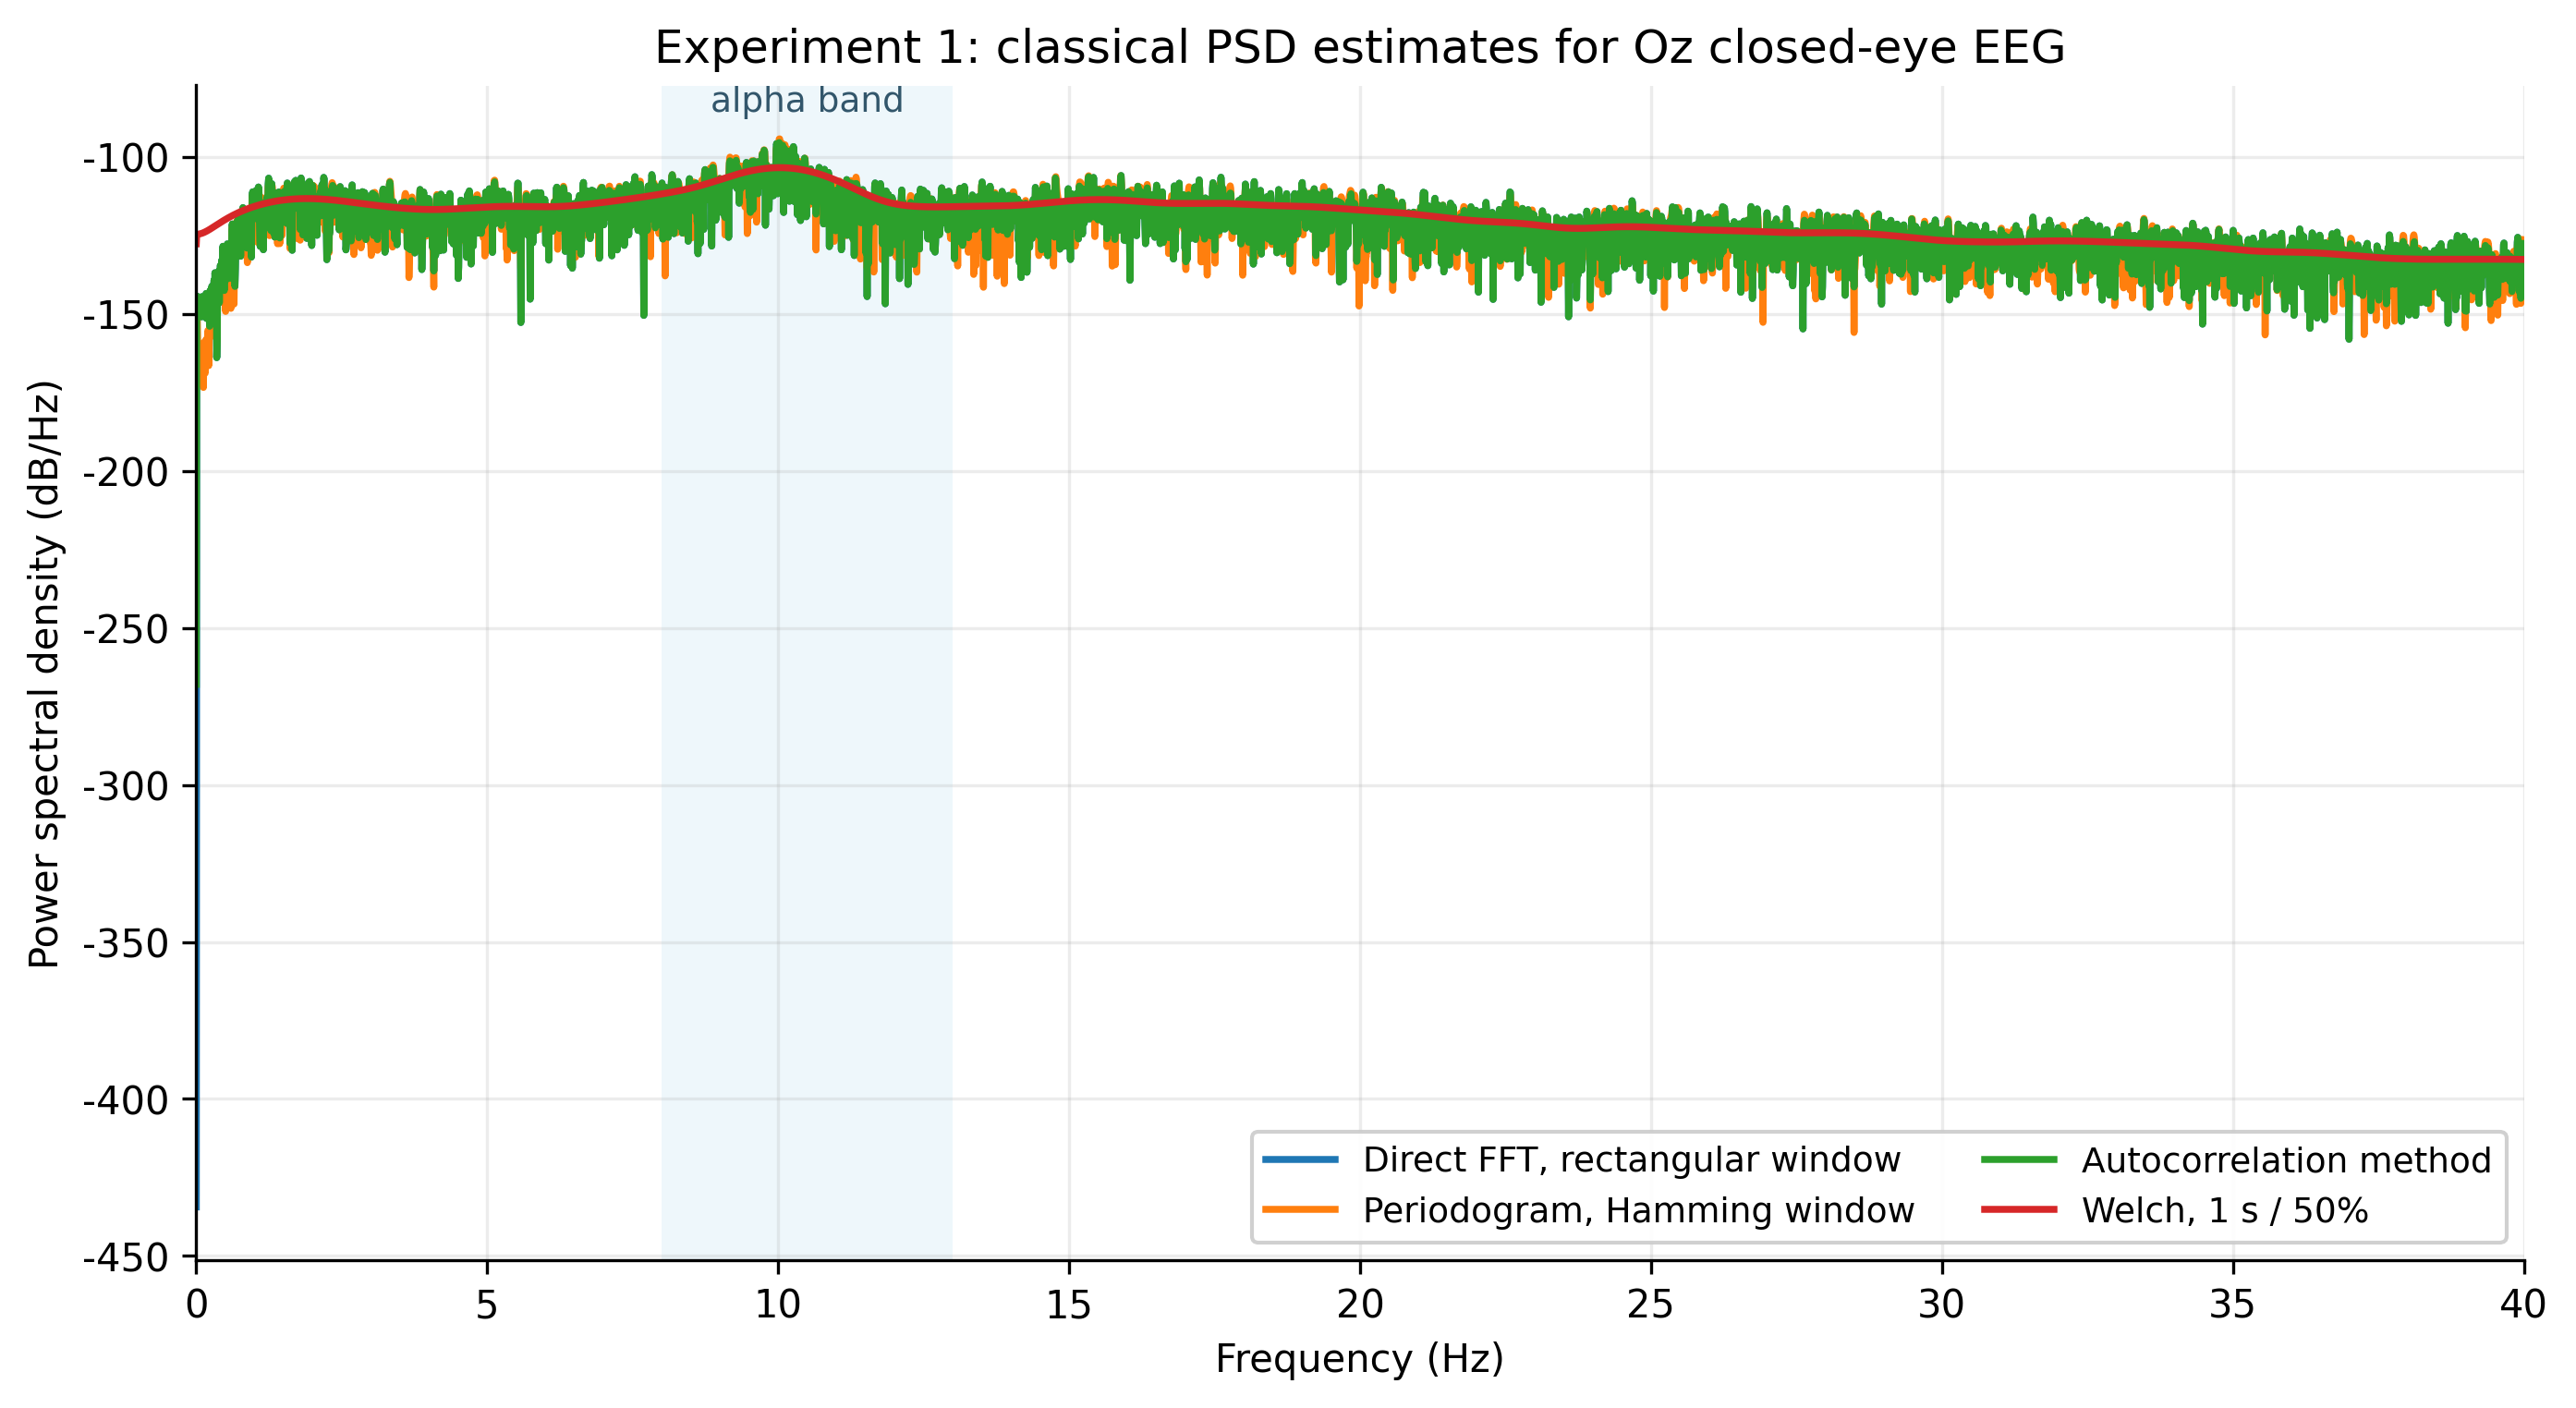
\includegraphics[width=\textwidth]{exp1_real_eeg_methods_en.png}
\caption{Four classical PSD estimates for the real Oz EEG segment.}
\end{figure}

\input{generated_en/table_exp1_real.tex}

\subsection{Discussion}
All methods identify the 12 Hz fundamental in the artificial signal. The 24 Hz harmonic is visible but more sensitive to smoothing and leakage. Welch produces a smoother curve by averaging segment periodograms, not because it knows the true spectrum better. The real EEG results show the same methodological dependence: alpha peak height, bandwidth, and background floor all change with estimator choice.

\textbf{Question: Why can the same closed-eye EEG segment yield different alpha peak shapes across estimators?}
Answer: A finite EEG segment is not a spectrum by itself. The estimator, window, averaging rule, and model assumptions determine leakage, variance, and smoothing, so they directly change peak height, bandwidth, and background-floor shape.

\textbf{Question: Does a smoother spectrum imply a more accurate spectrum?}
Answer: No. Smoothness usually means lower variance, often bought by bias or reduced resolution. A smoothed spectrum can suppress a real narrow component or hide transient structure.

\section{Experiment 2: Leakage, Resolution, and NFFT}

\subsection{Synthetic Signals}
For length-resolution analysis, the signal is $\sin(2\pi10t)+0.8\sin(2\pi11t)$ with record lengths 1, 2, 4, and 8 s. For leakage analysis, the signal is $\sin(2\pi10.3t)+0.15\sin(2\pi14.1t)$ with length 1.8 s. For the NFFT experiment, the signal is $\sin(2\pi10t)+0.8\sin(2\pi10.4t)$ with length 1 s and varying NFFT.

\begin{figure}[H]
\centering
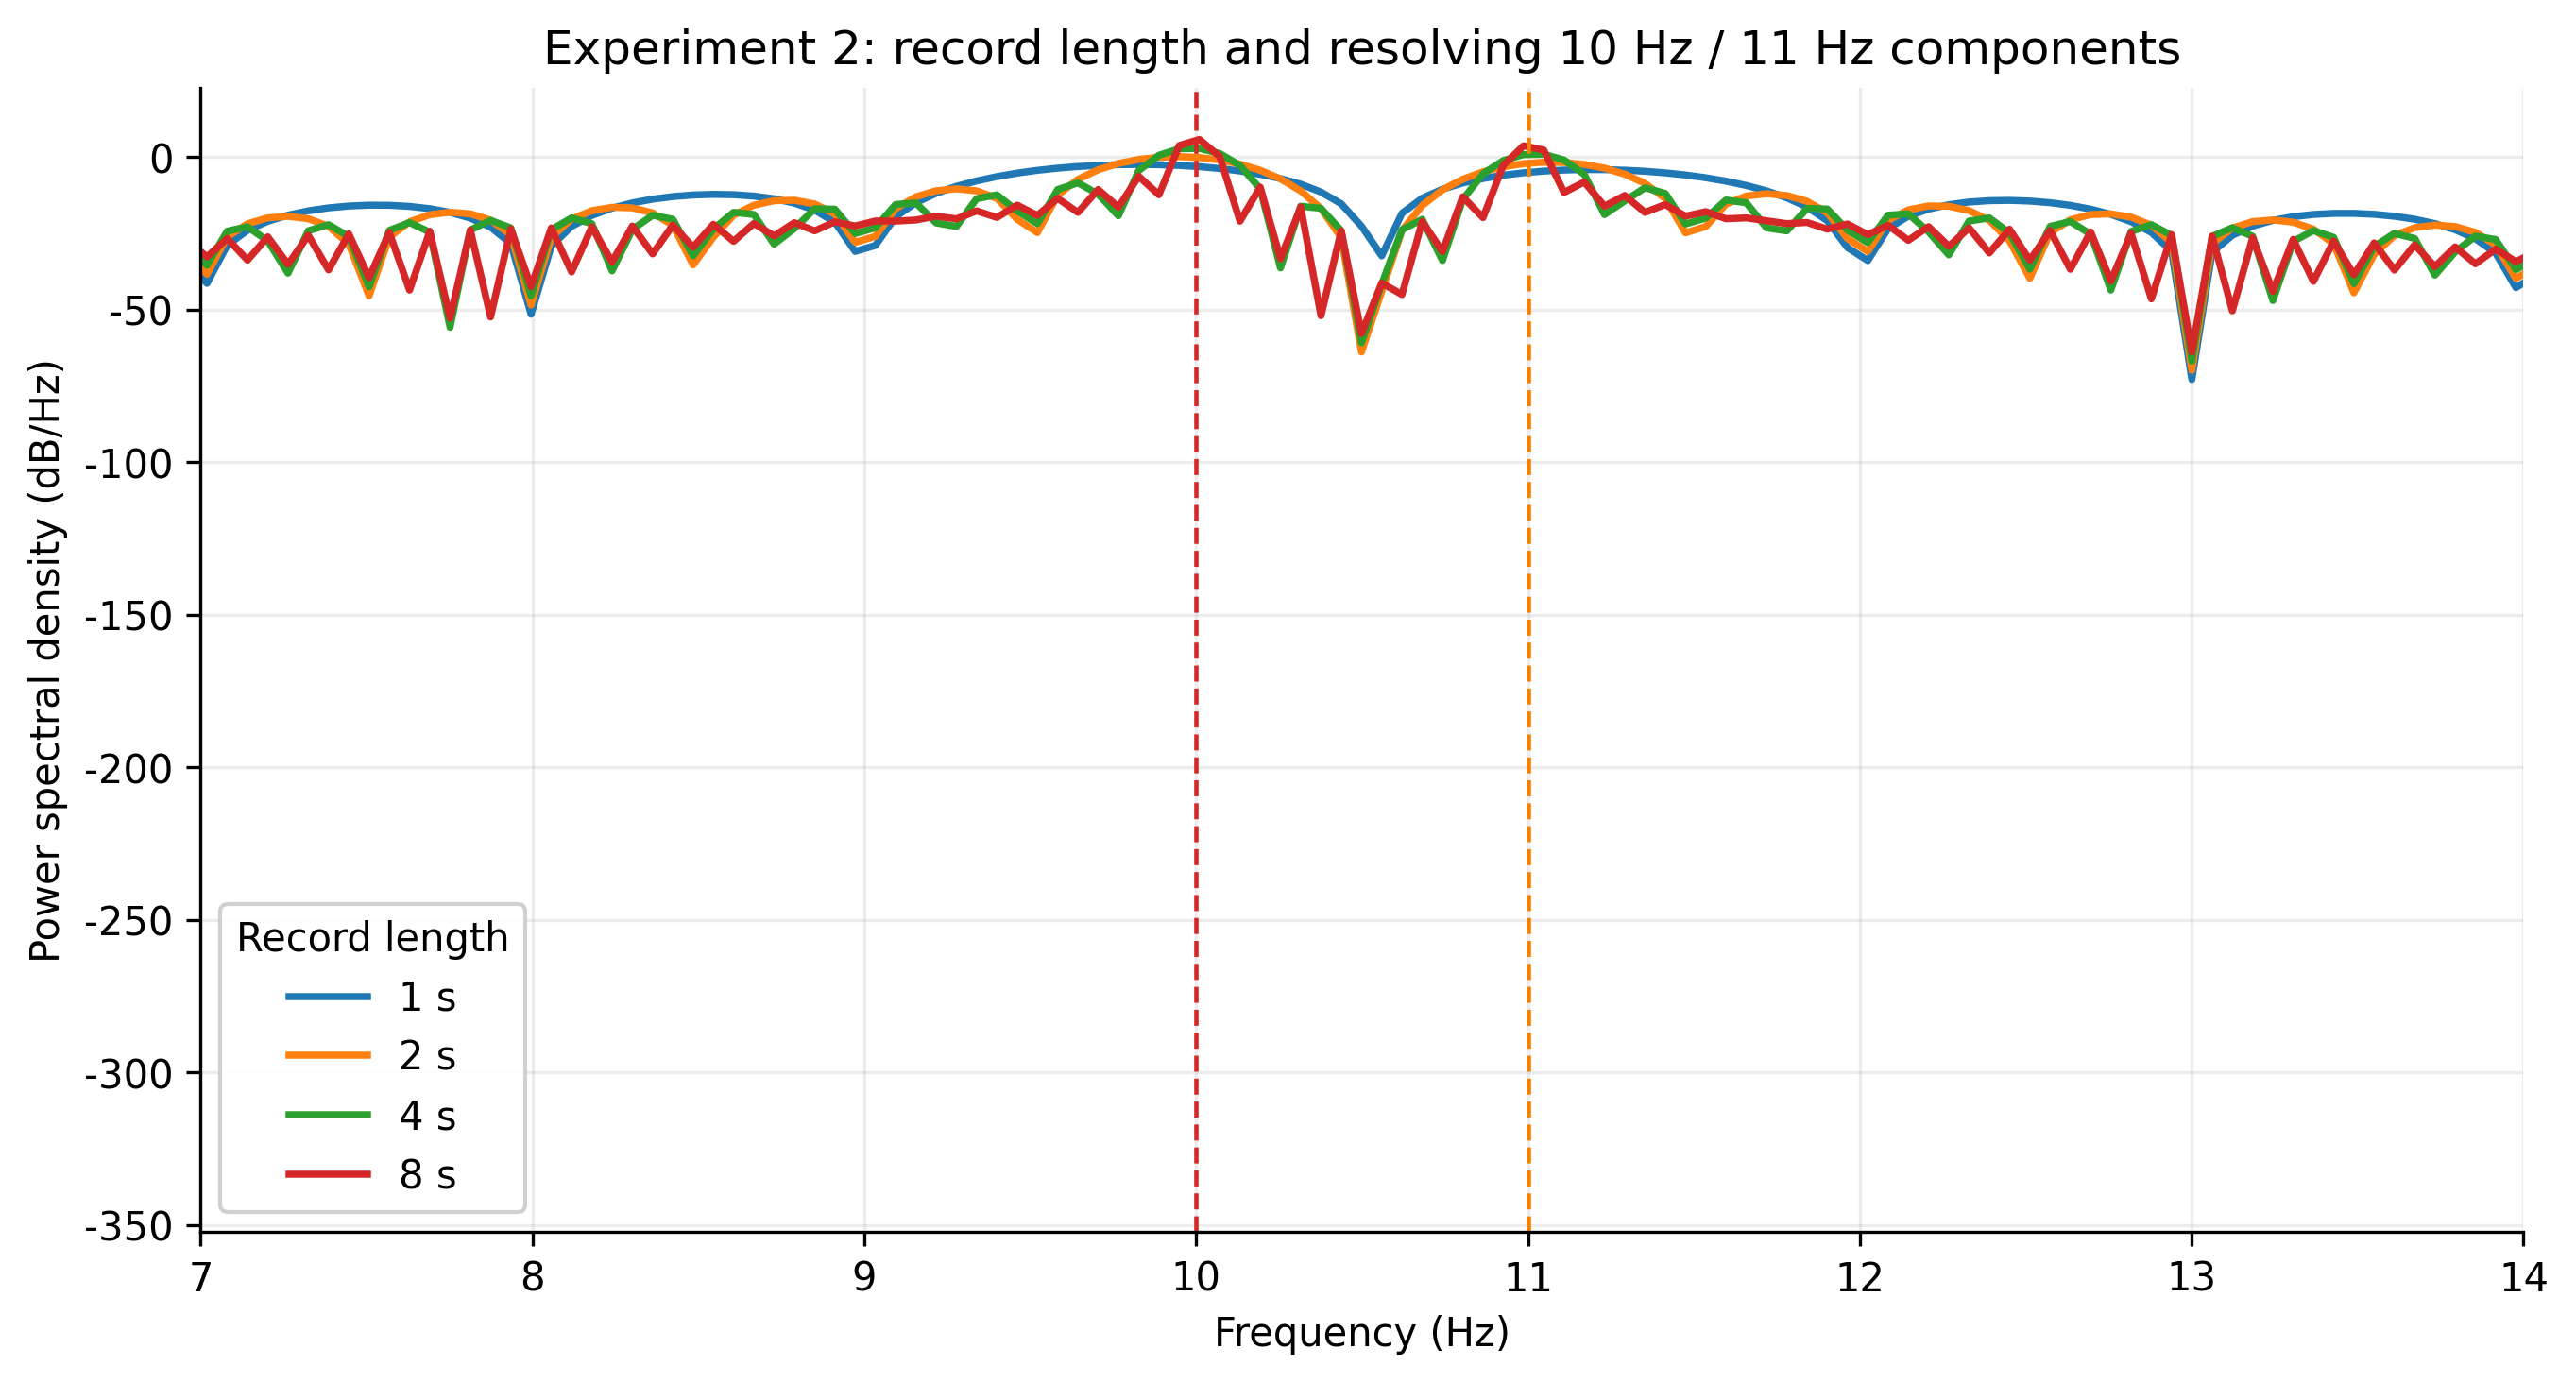
\includegraphics[width=\textwidth]{exp2_length_resolution_en.png}
\caption{Record length controls the ability to separate 10 Hz and 11 Hz components.}
\end{figure}

\input{generated_en/table_exp2_length.tex}

\begin{figure}[H]
\centering
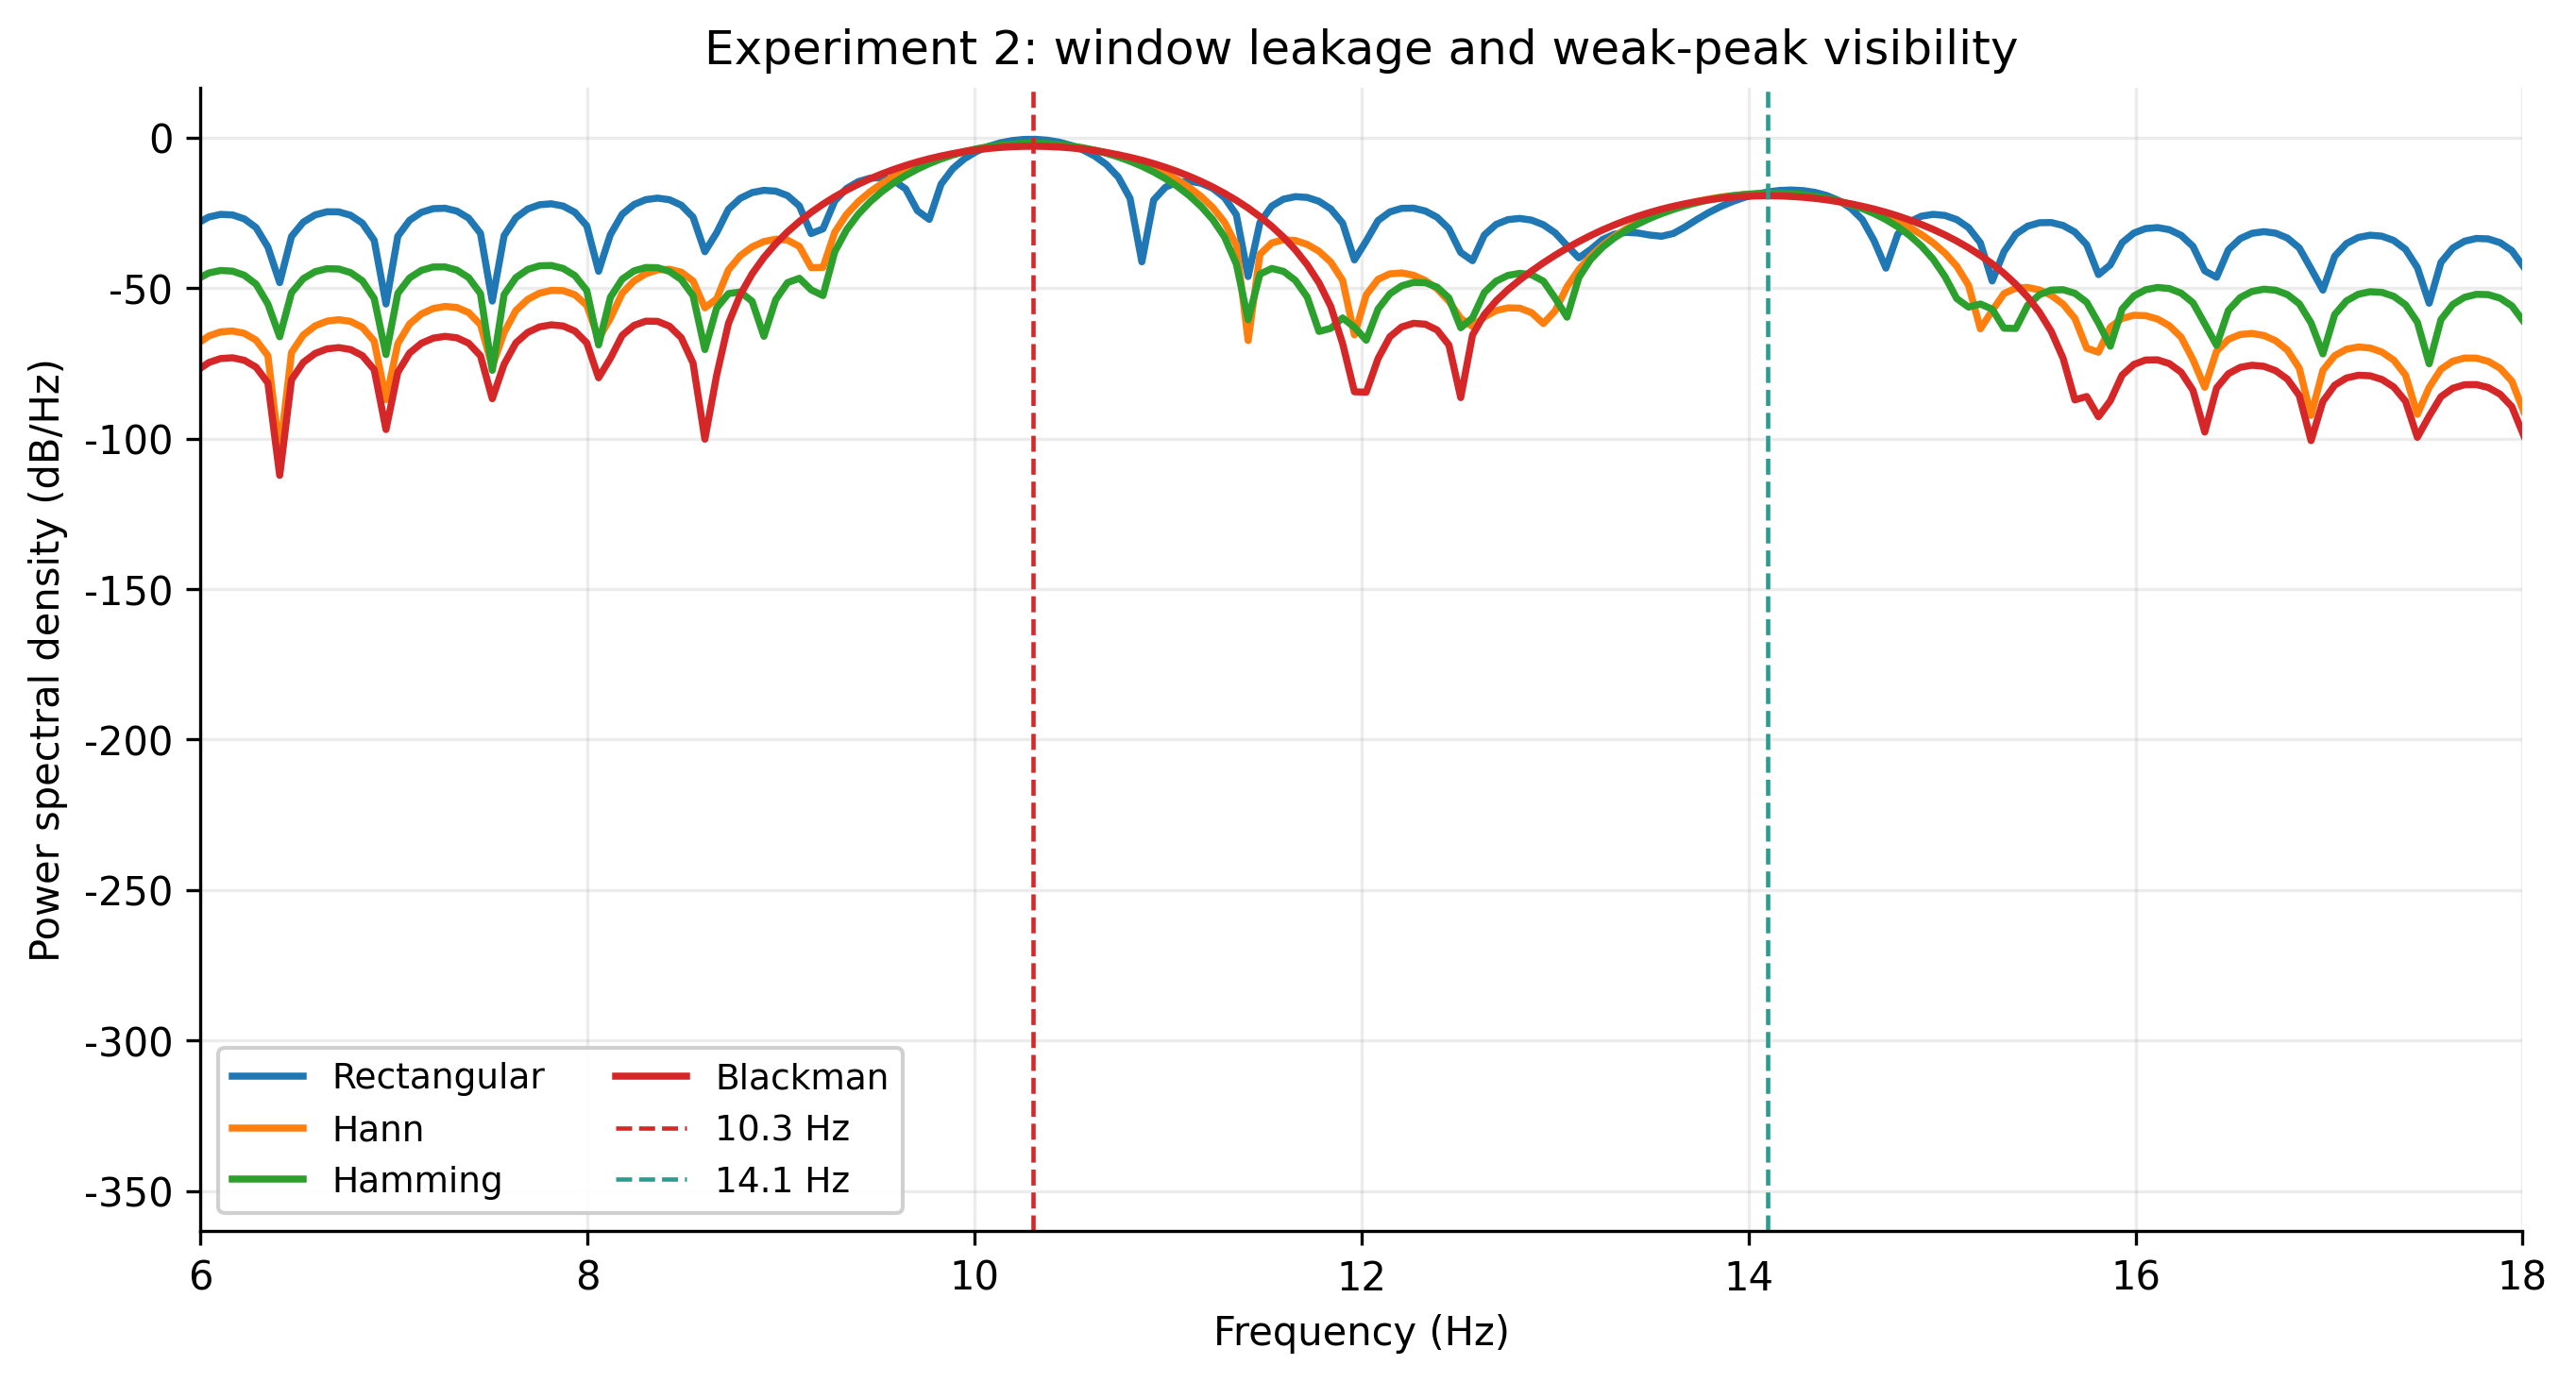
\includegraphics[width=\textwidth]{exp2_window_leakage_en.png}
\caption{Window choice changes sidelobe leakage and main-lobe width.}
\end{figure}

\input{generated_en/table_exp2_window.tex}

\begin{figure}[H]
\centering
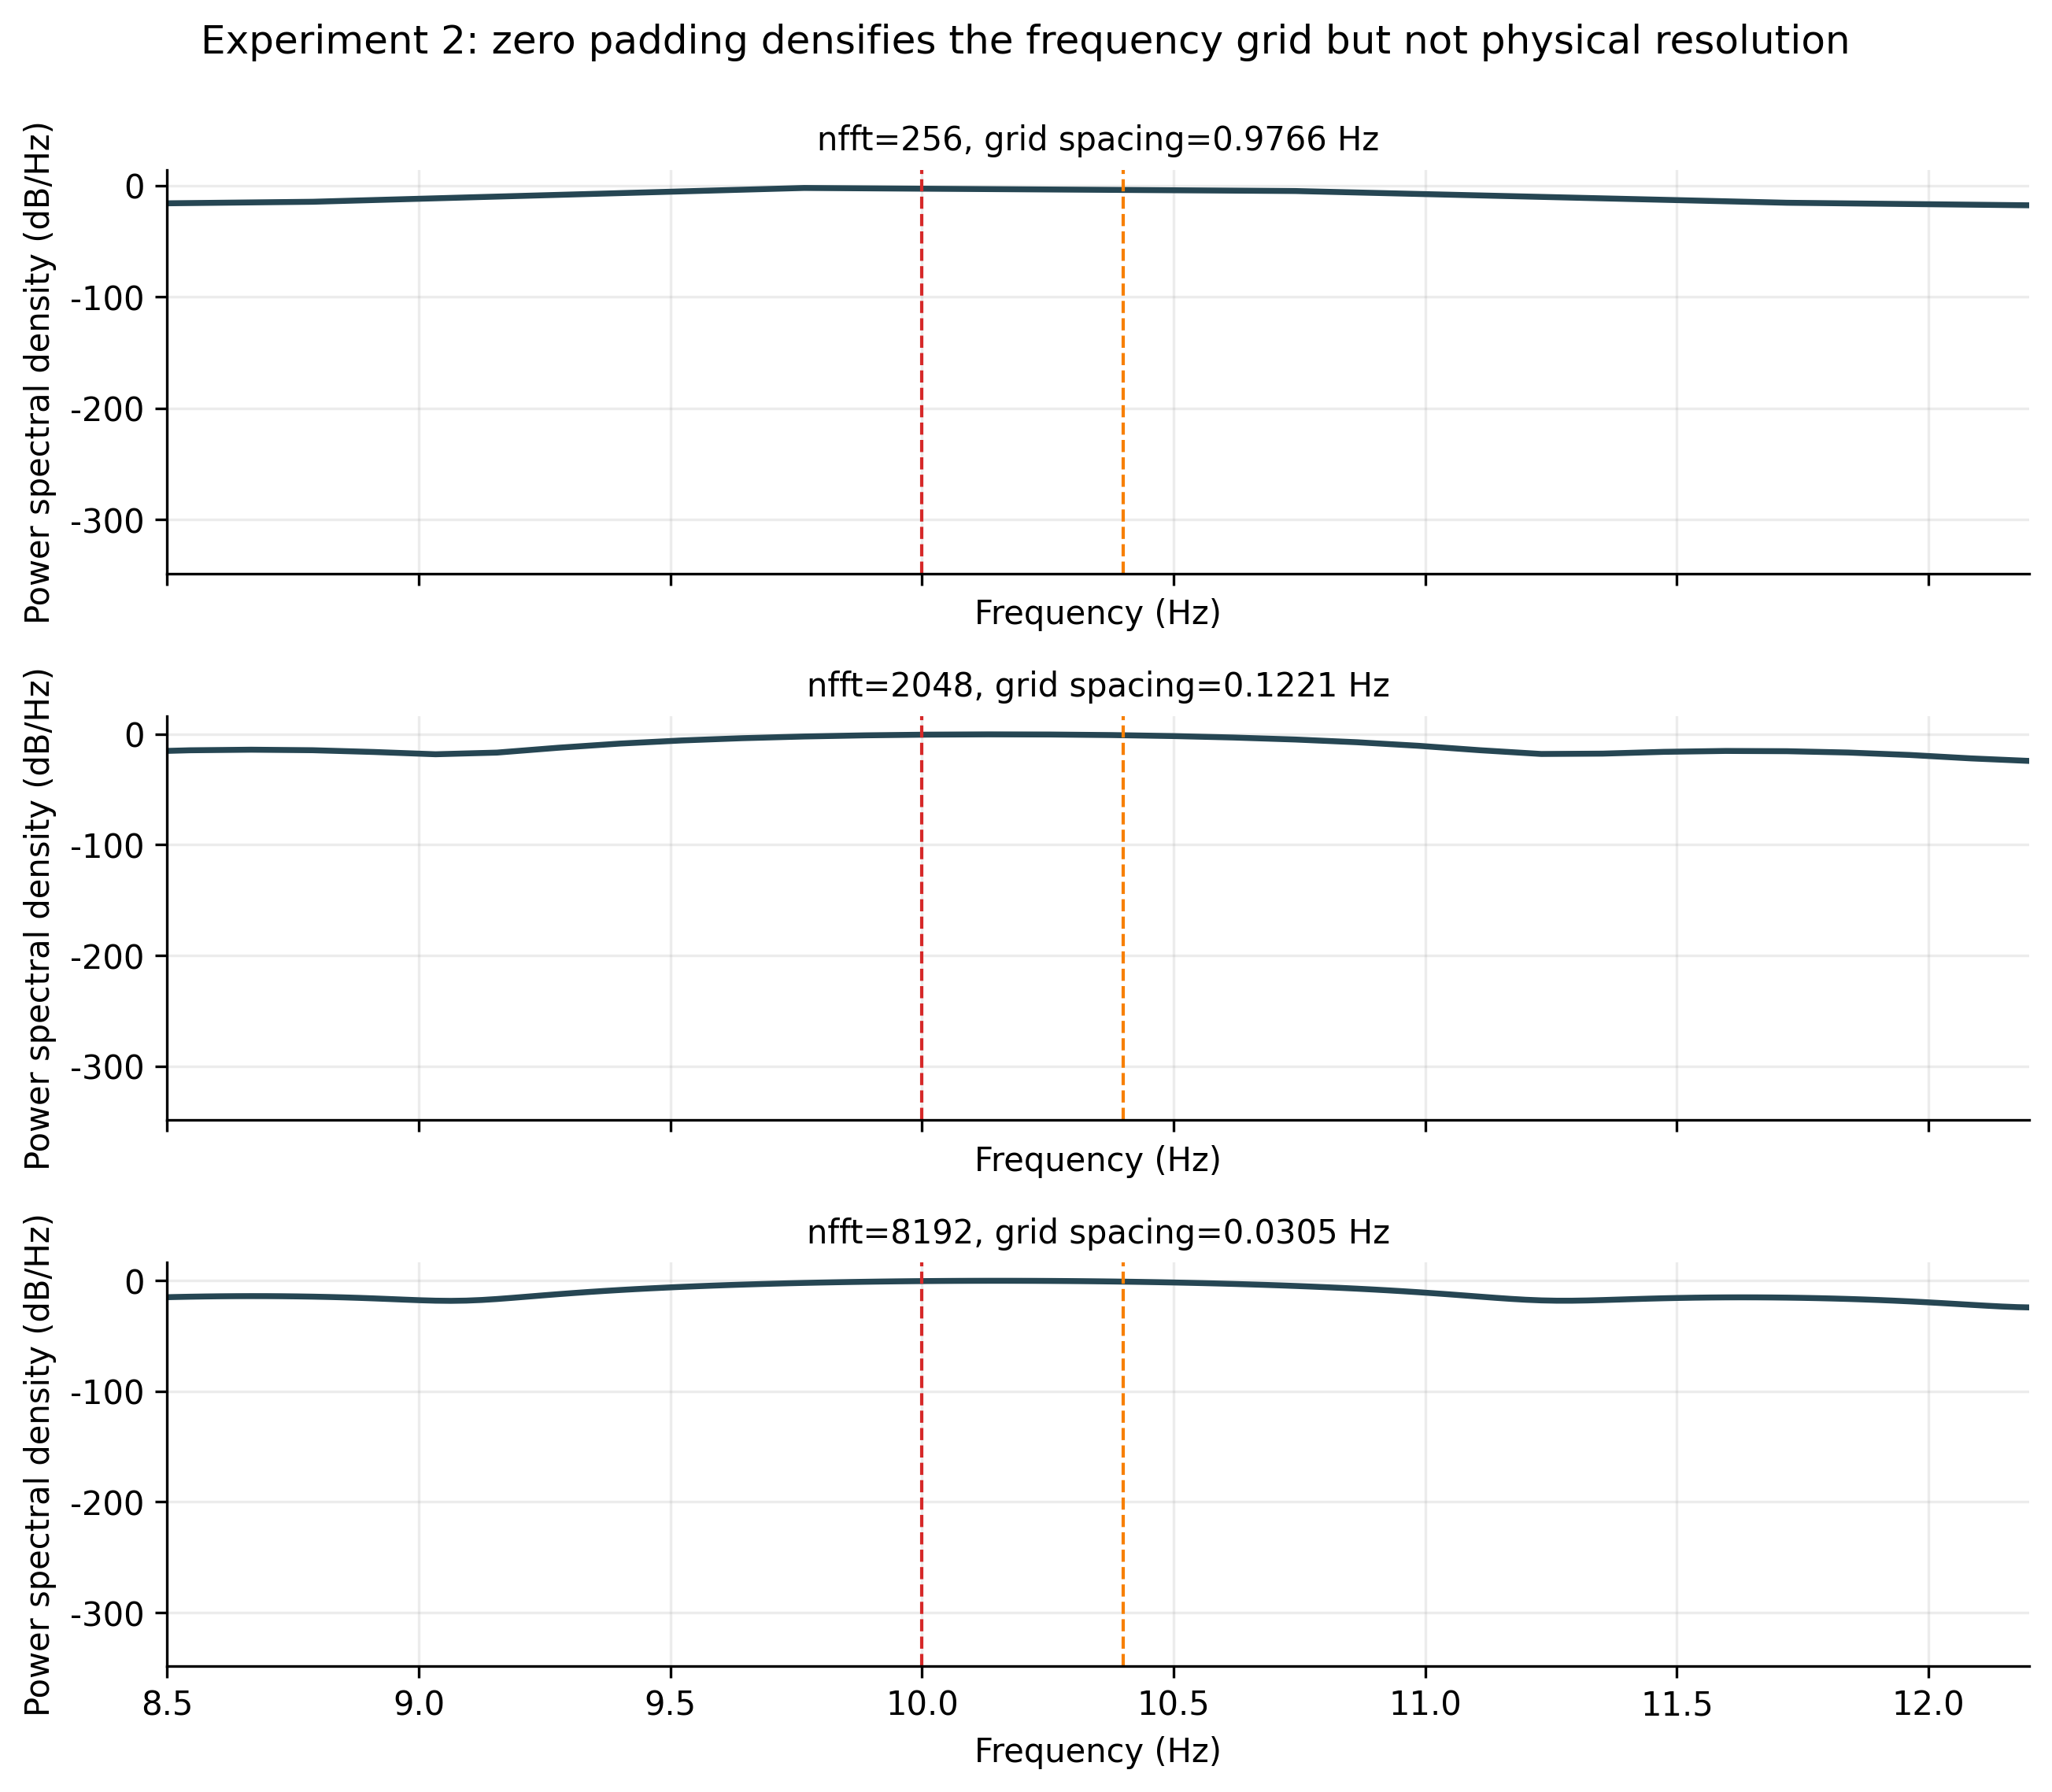
\includegraphics[width=\textwidth]{exp2_nfft_subplots_en.png}
\caption{Increasing NFFT densifies the plotted frequency grid but does not overcome the 1 s observation length.}
\end{figure}

\input{generated_en/table_exp2_nfft.tex}

\subsection{Real EEG}
The same ideas are tested on the real Oz EEG segment. The 10, 30, and 59 s comparisons isolate record length; the window comparison uses the same 30 s segment and NFFT 8192; the NFFT comparison keeps the same 30 s segment while using 7500, 15000, and 30000 FFT points.

\begin{figure}[H]
\centering
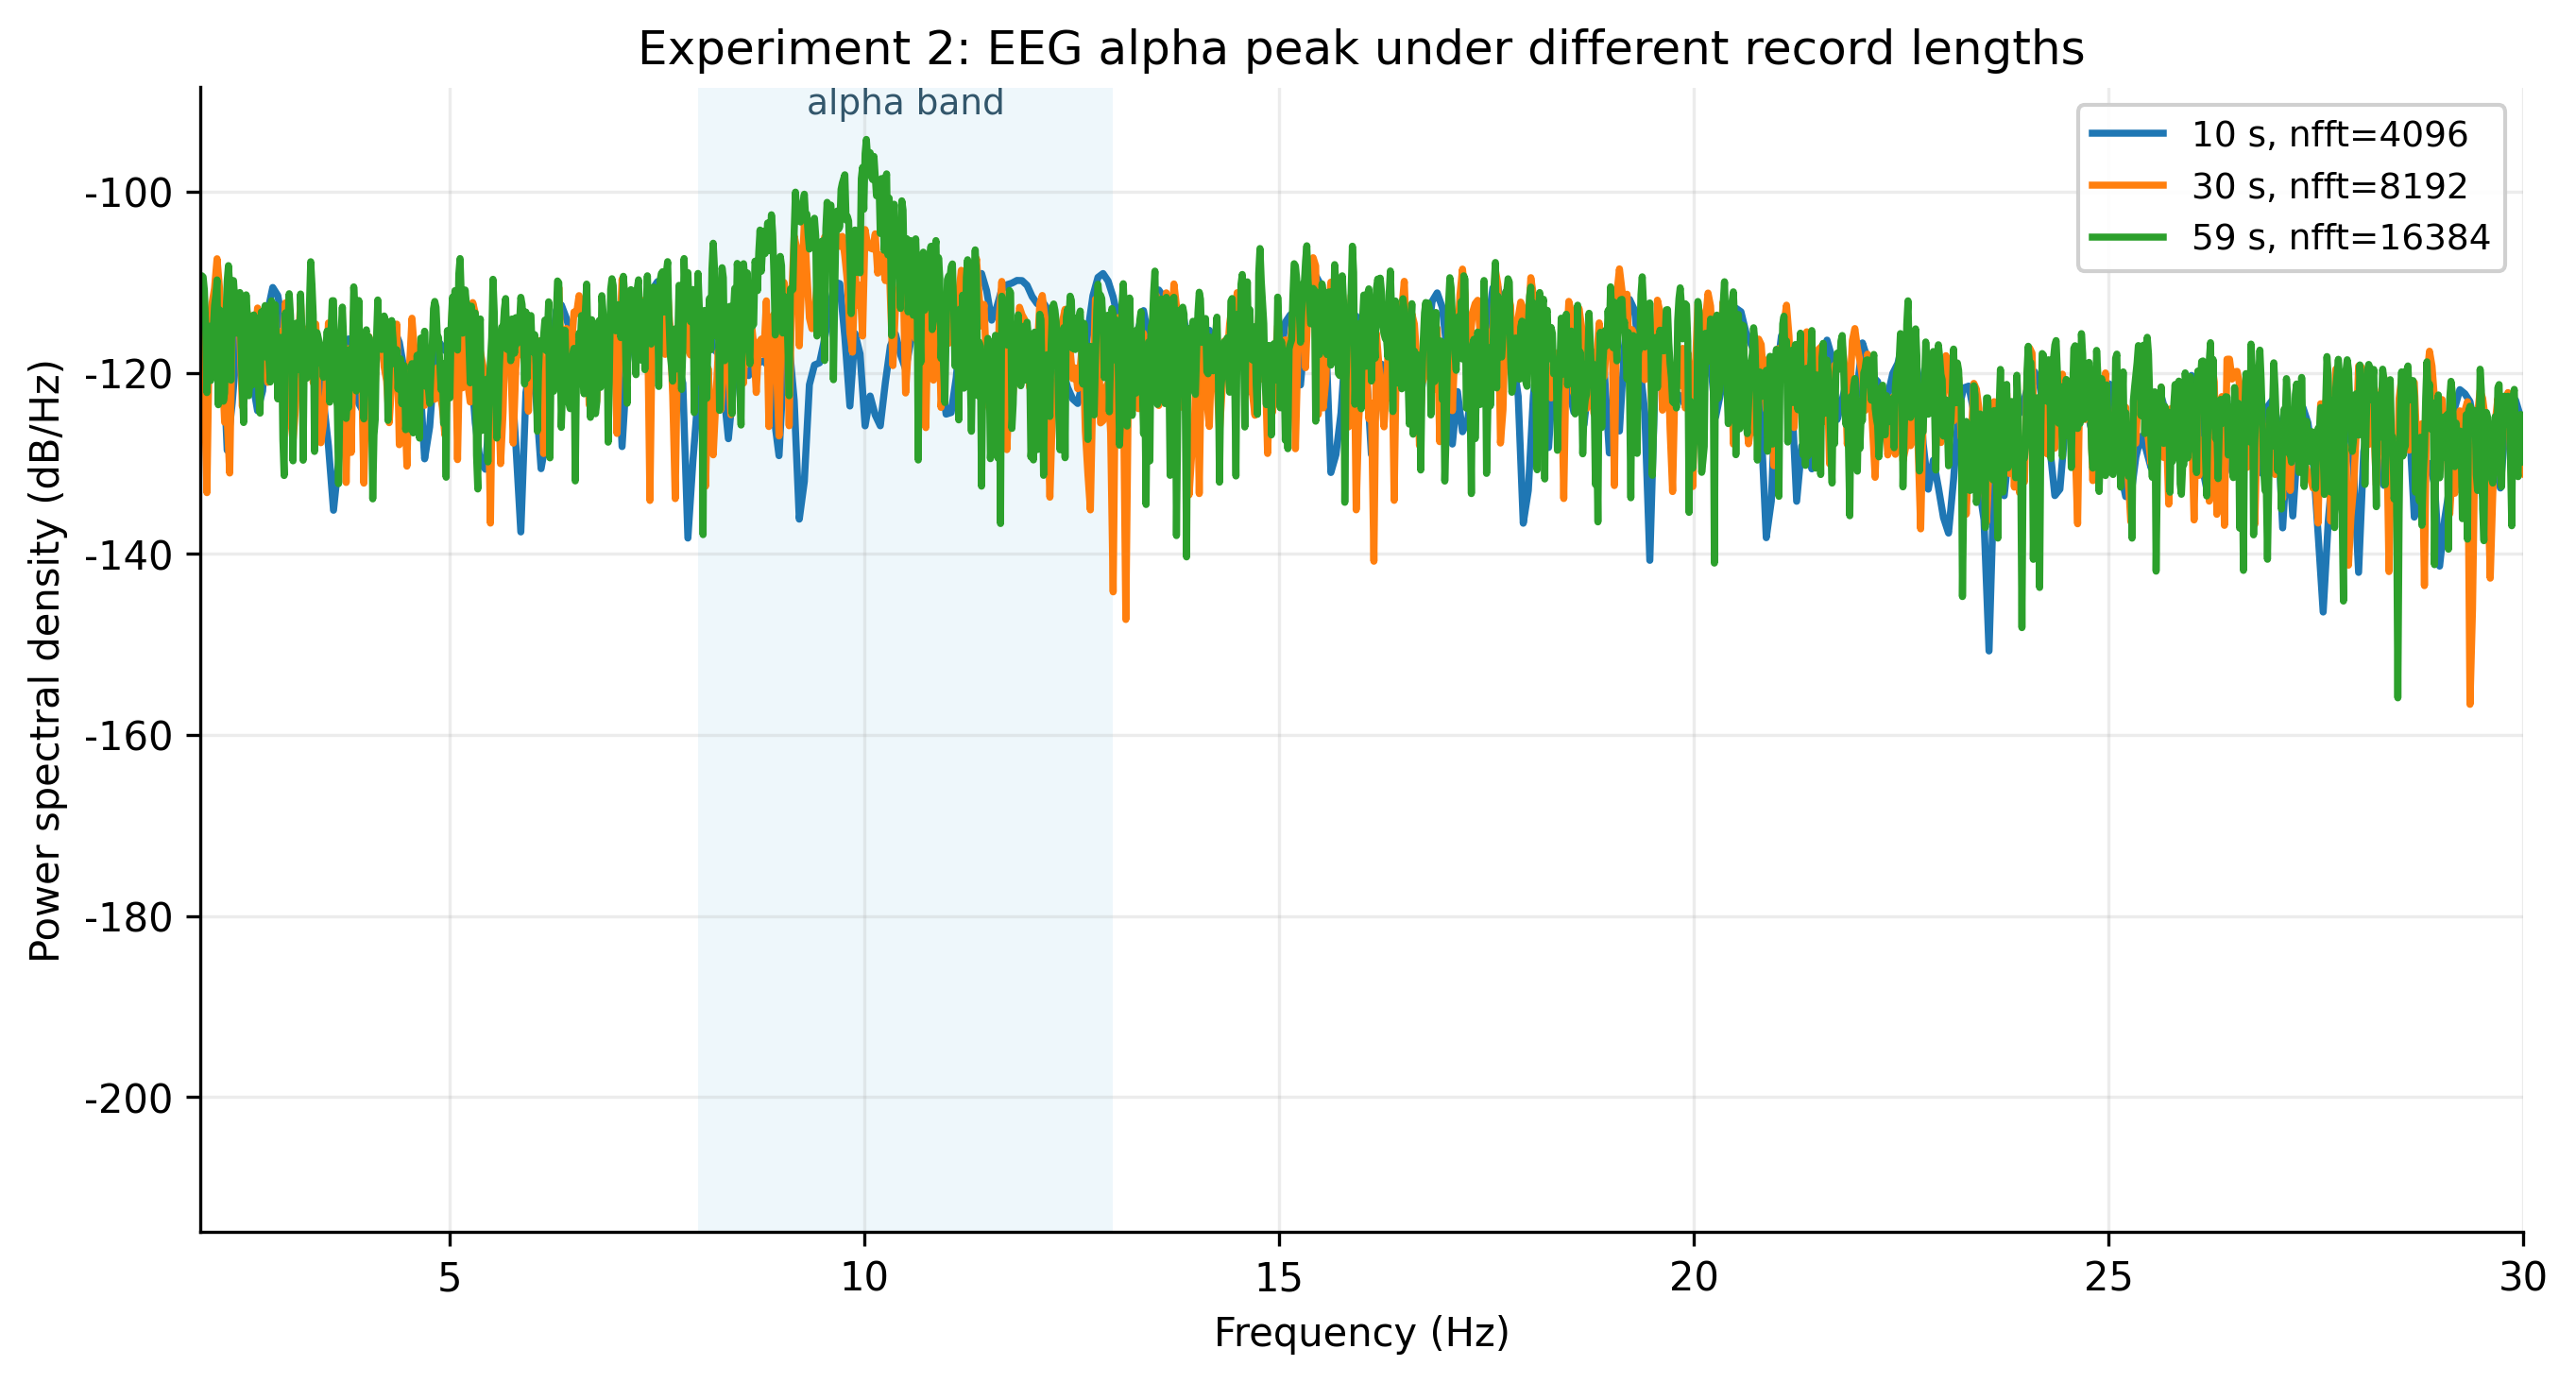
\includegraphics[width=\textwidth]{exp2_real_length_alpha_en.png}
\caption{Real EEG alpha shape under different record lengths.}
\end{figure}

\input{generated_en/table_exp2_real_length.tex}

\begin{figure}[H]
\centering
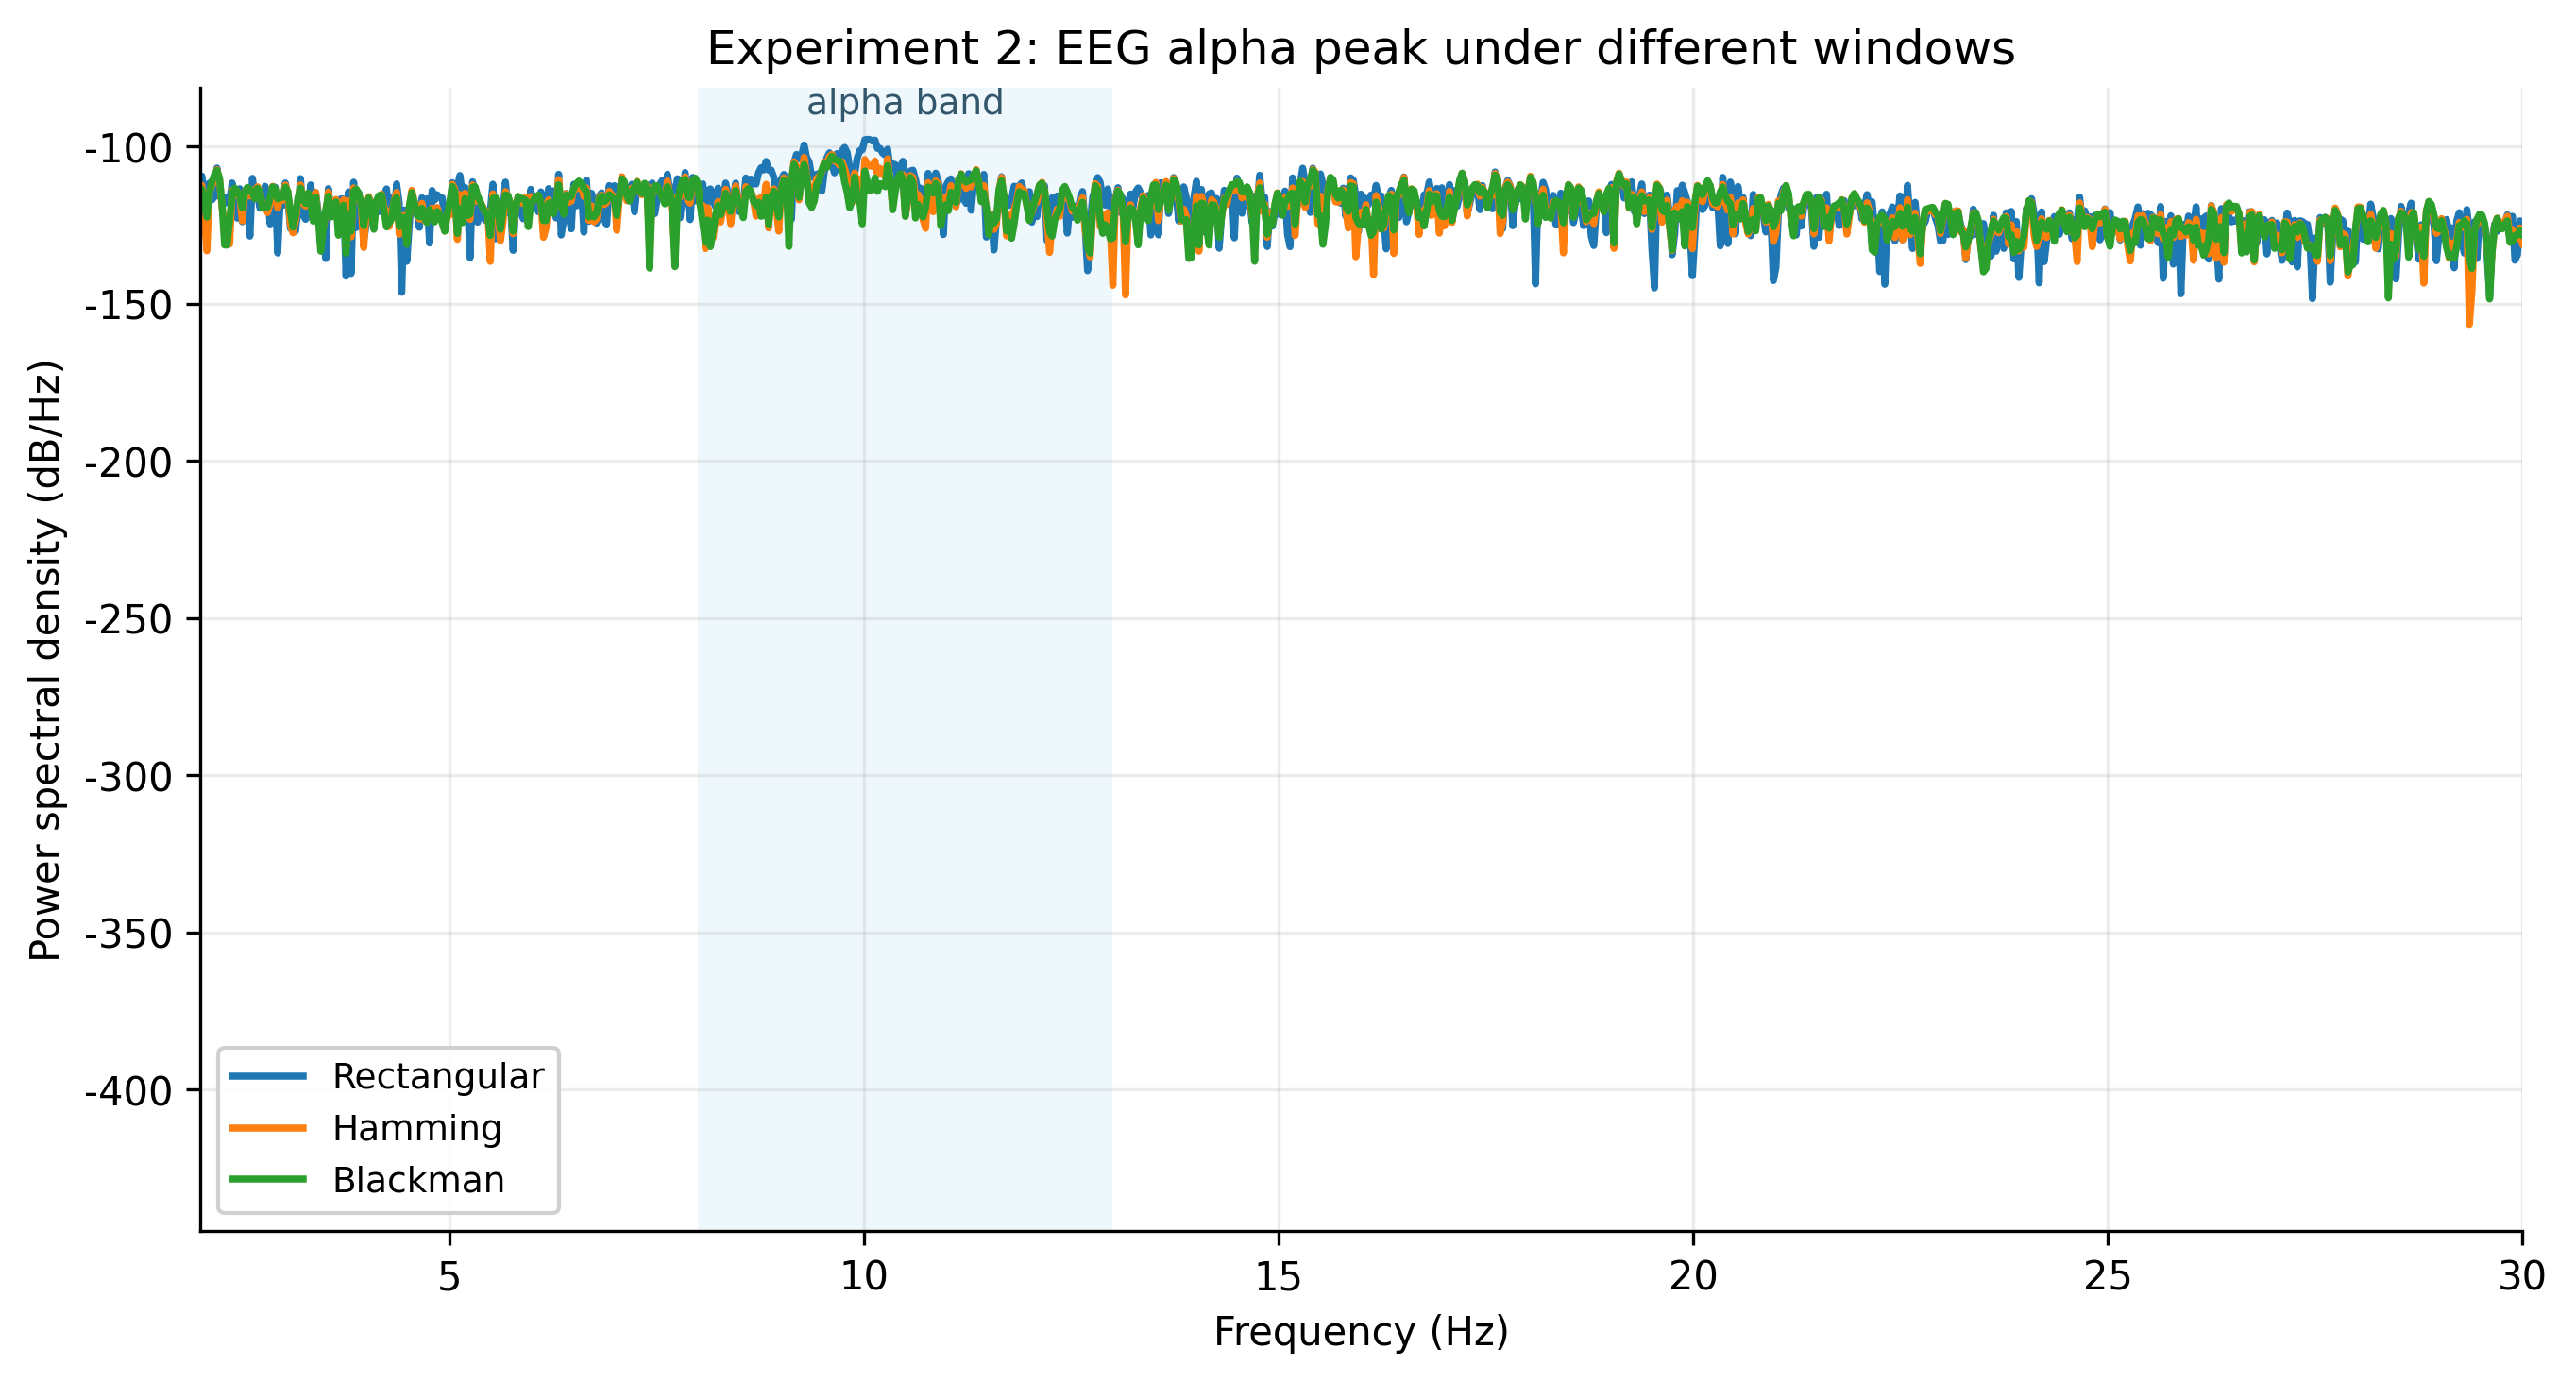
\includegraphics[width=\textwidth]{exp2_real_windows_alpha_en.png}
\caption{Real EEG alpha shape under different windows.}
\end{figure}

\input{generated_en/table_exp2_real_window.tex}

\begin{figure}[H]
\centering
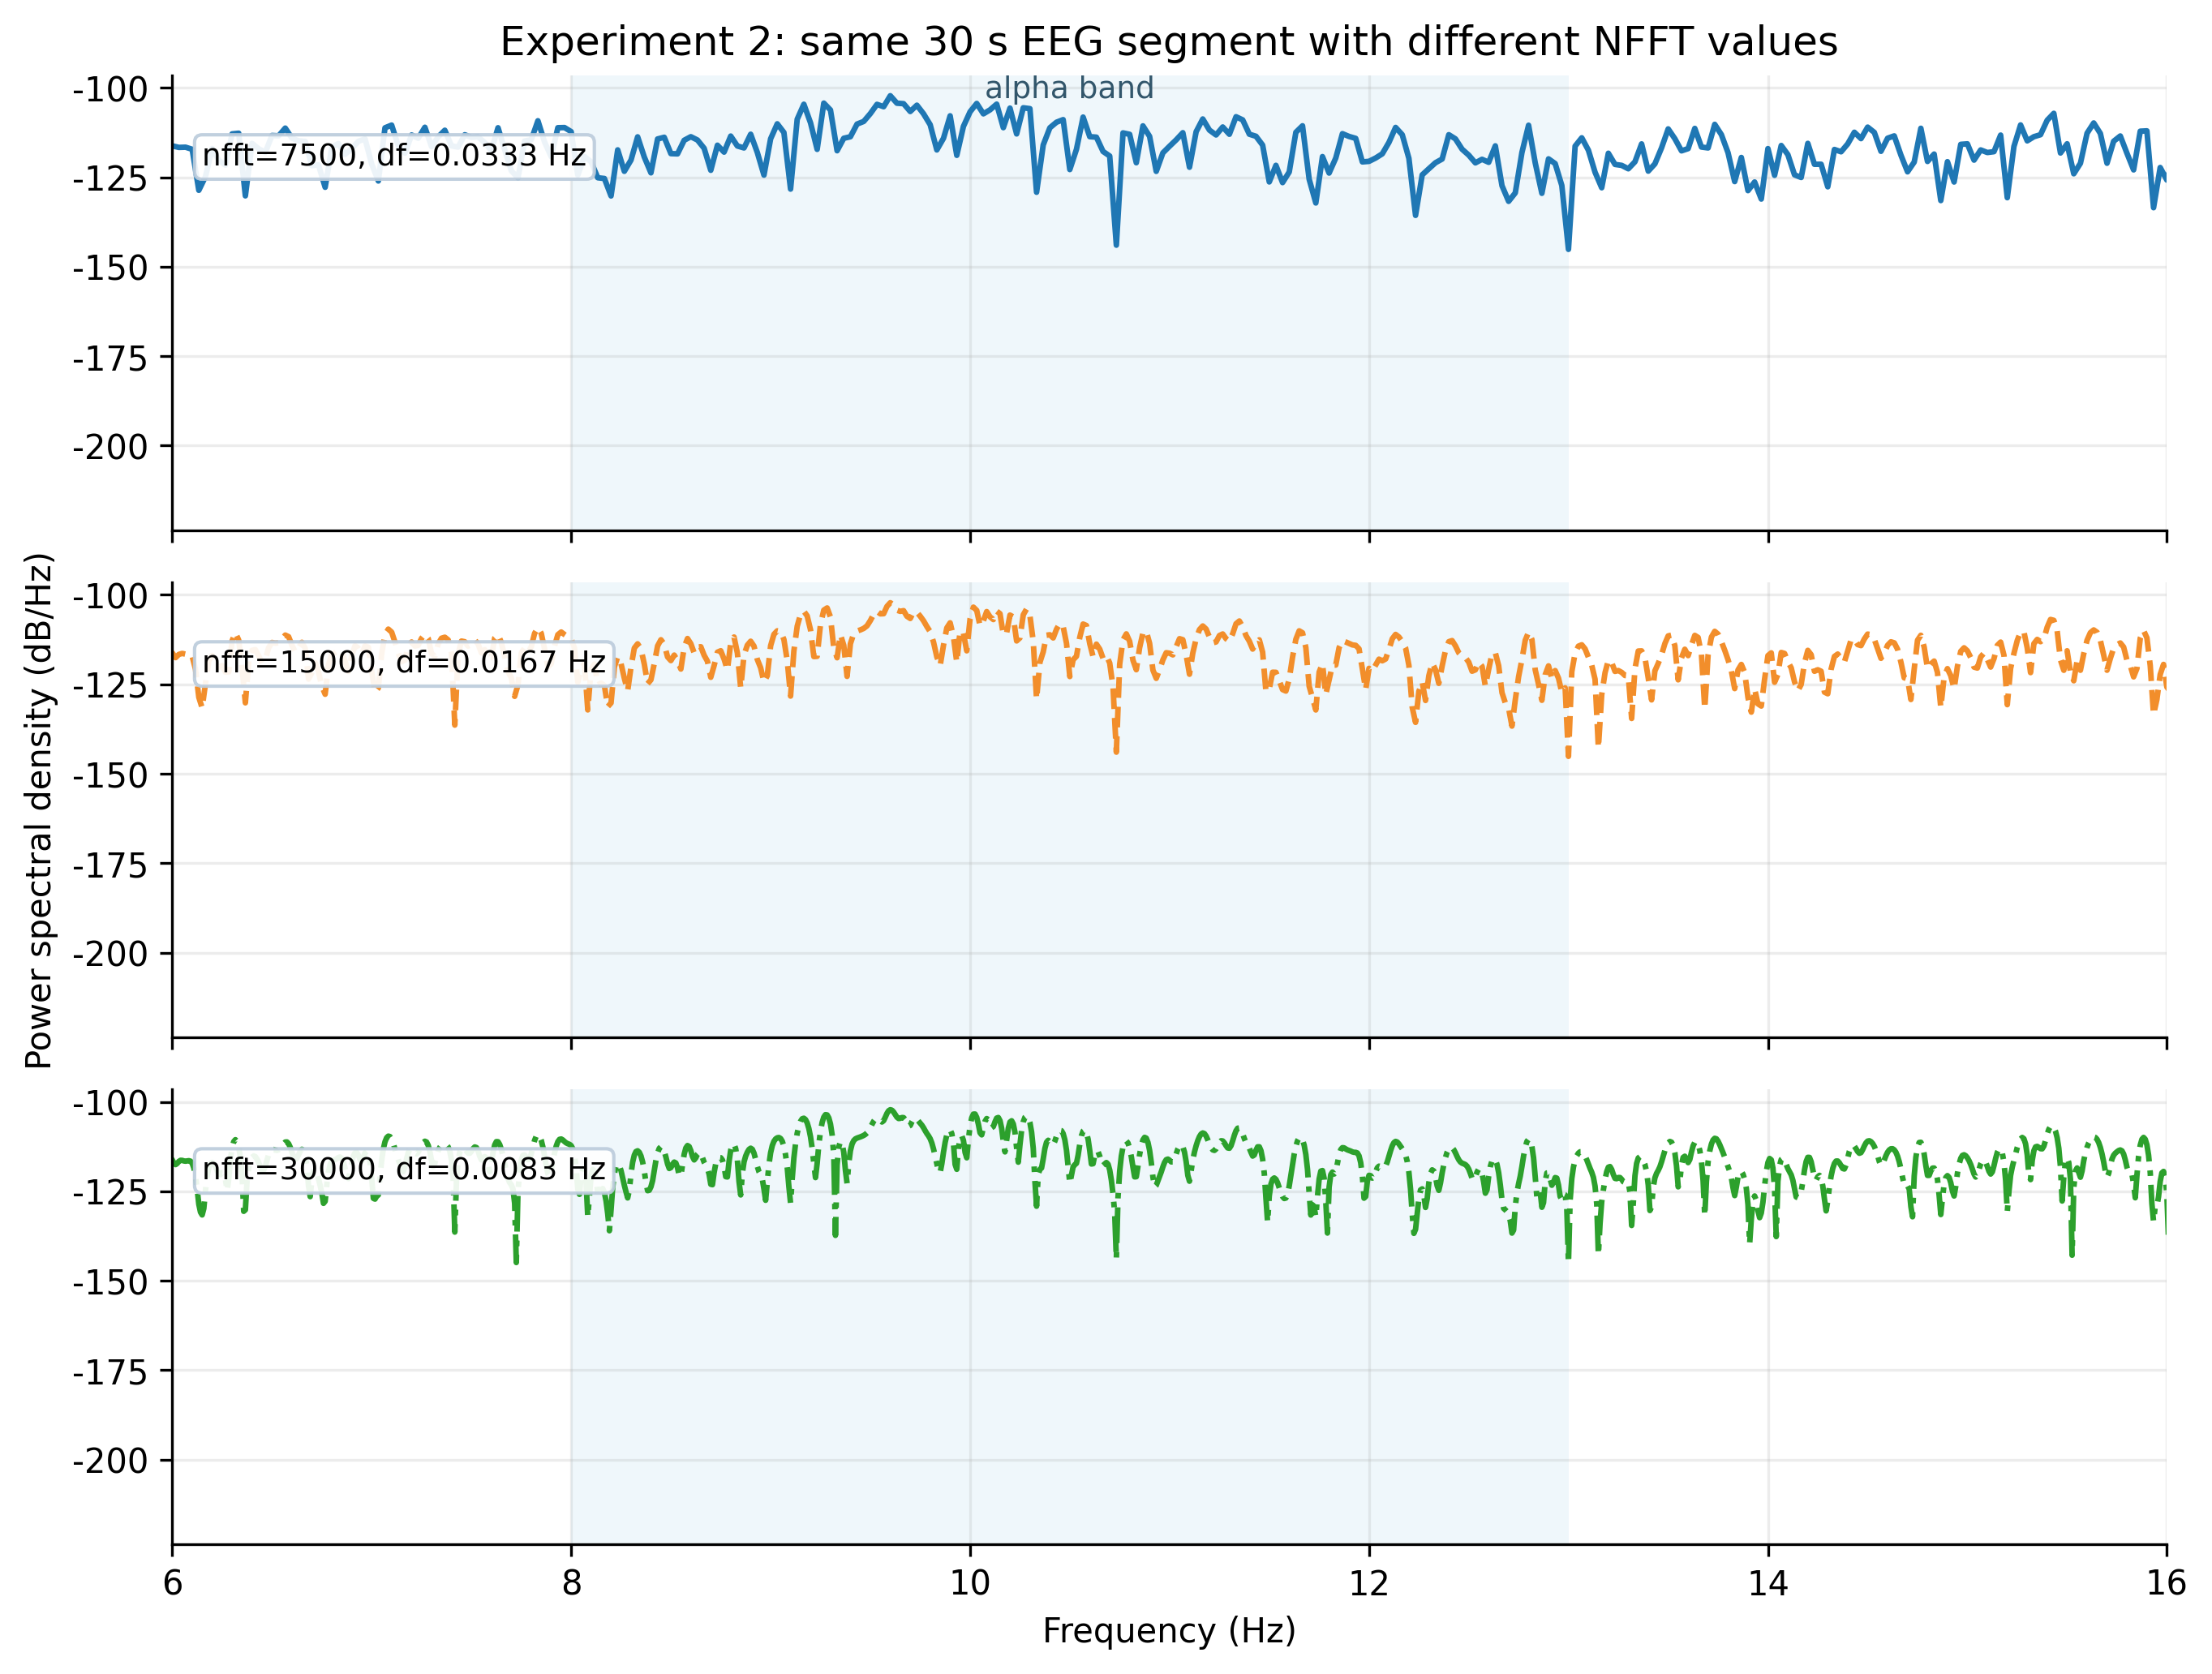
\includegraphics[width=\textwidth]{exp2_real_nfft_alpha_en.png}
\caption{Same 30 s EEG segment with different NFFT values.}
\end{figure}

\input{generated_en/table_exp2_real_nfft.tex}

\subsection{Discussion}
Longer records reduce the Rayleigh interval $1/T$ and narrow the main lobe, making close frequencies easier to separate. Low-sidelobe windows reduce leakage from a strong component into nearby frequencies but widen the main lobe, so leakage suppression and resolution are not free at the same time. Zero padding increases the number of frequency samples; it does not add observations and therefore does not increase physical resolution.

\textbf{Question: Why can increasing record length solve resolution problems while increasing NFFT usually cannot?}
Answer: Record length changes the information content and Rayleigh spacing. NFFT changes interpolation density on the same finite-data Fourier transform.

\textbf{Question: Why are high resolution, low leakage, and smoothness hard to optimize simultaneously?}
Answer: They map to competing design choices: long records improve resolution, low-sidelobe windows widen peaks, and averaging reduces variance at the cost of short-segment resolution.

\section{Experiment 3: Welch Versus AR Spectral Estimation}

\subsection{Synthetic Signal and AR Order Selection}
The artificial signal is
\[
x(t)=\sin(2\pi10t)+0.8\sin(2\pi11t)+w(t),
\]
with 2 s duration. Welch uses 1 s segments, 50\% overlap, and a Hamming window. AR spectra use Yule-Walker estimation with representative orders $p=4,16,32,128$, and FPE is scanned over $p=2,\ldots,30$.

\begin{figure}[H]
\centering
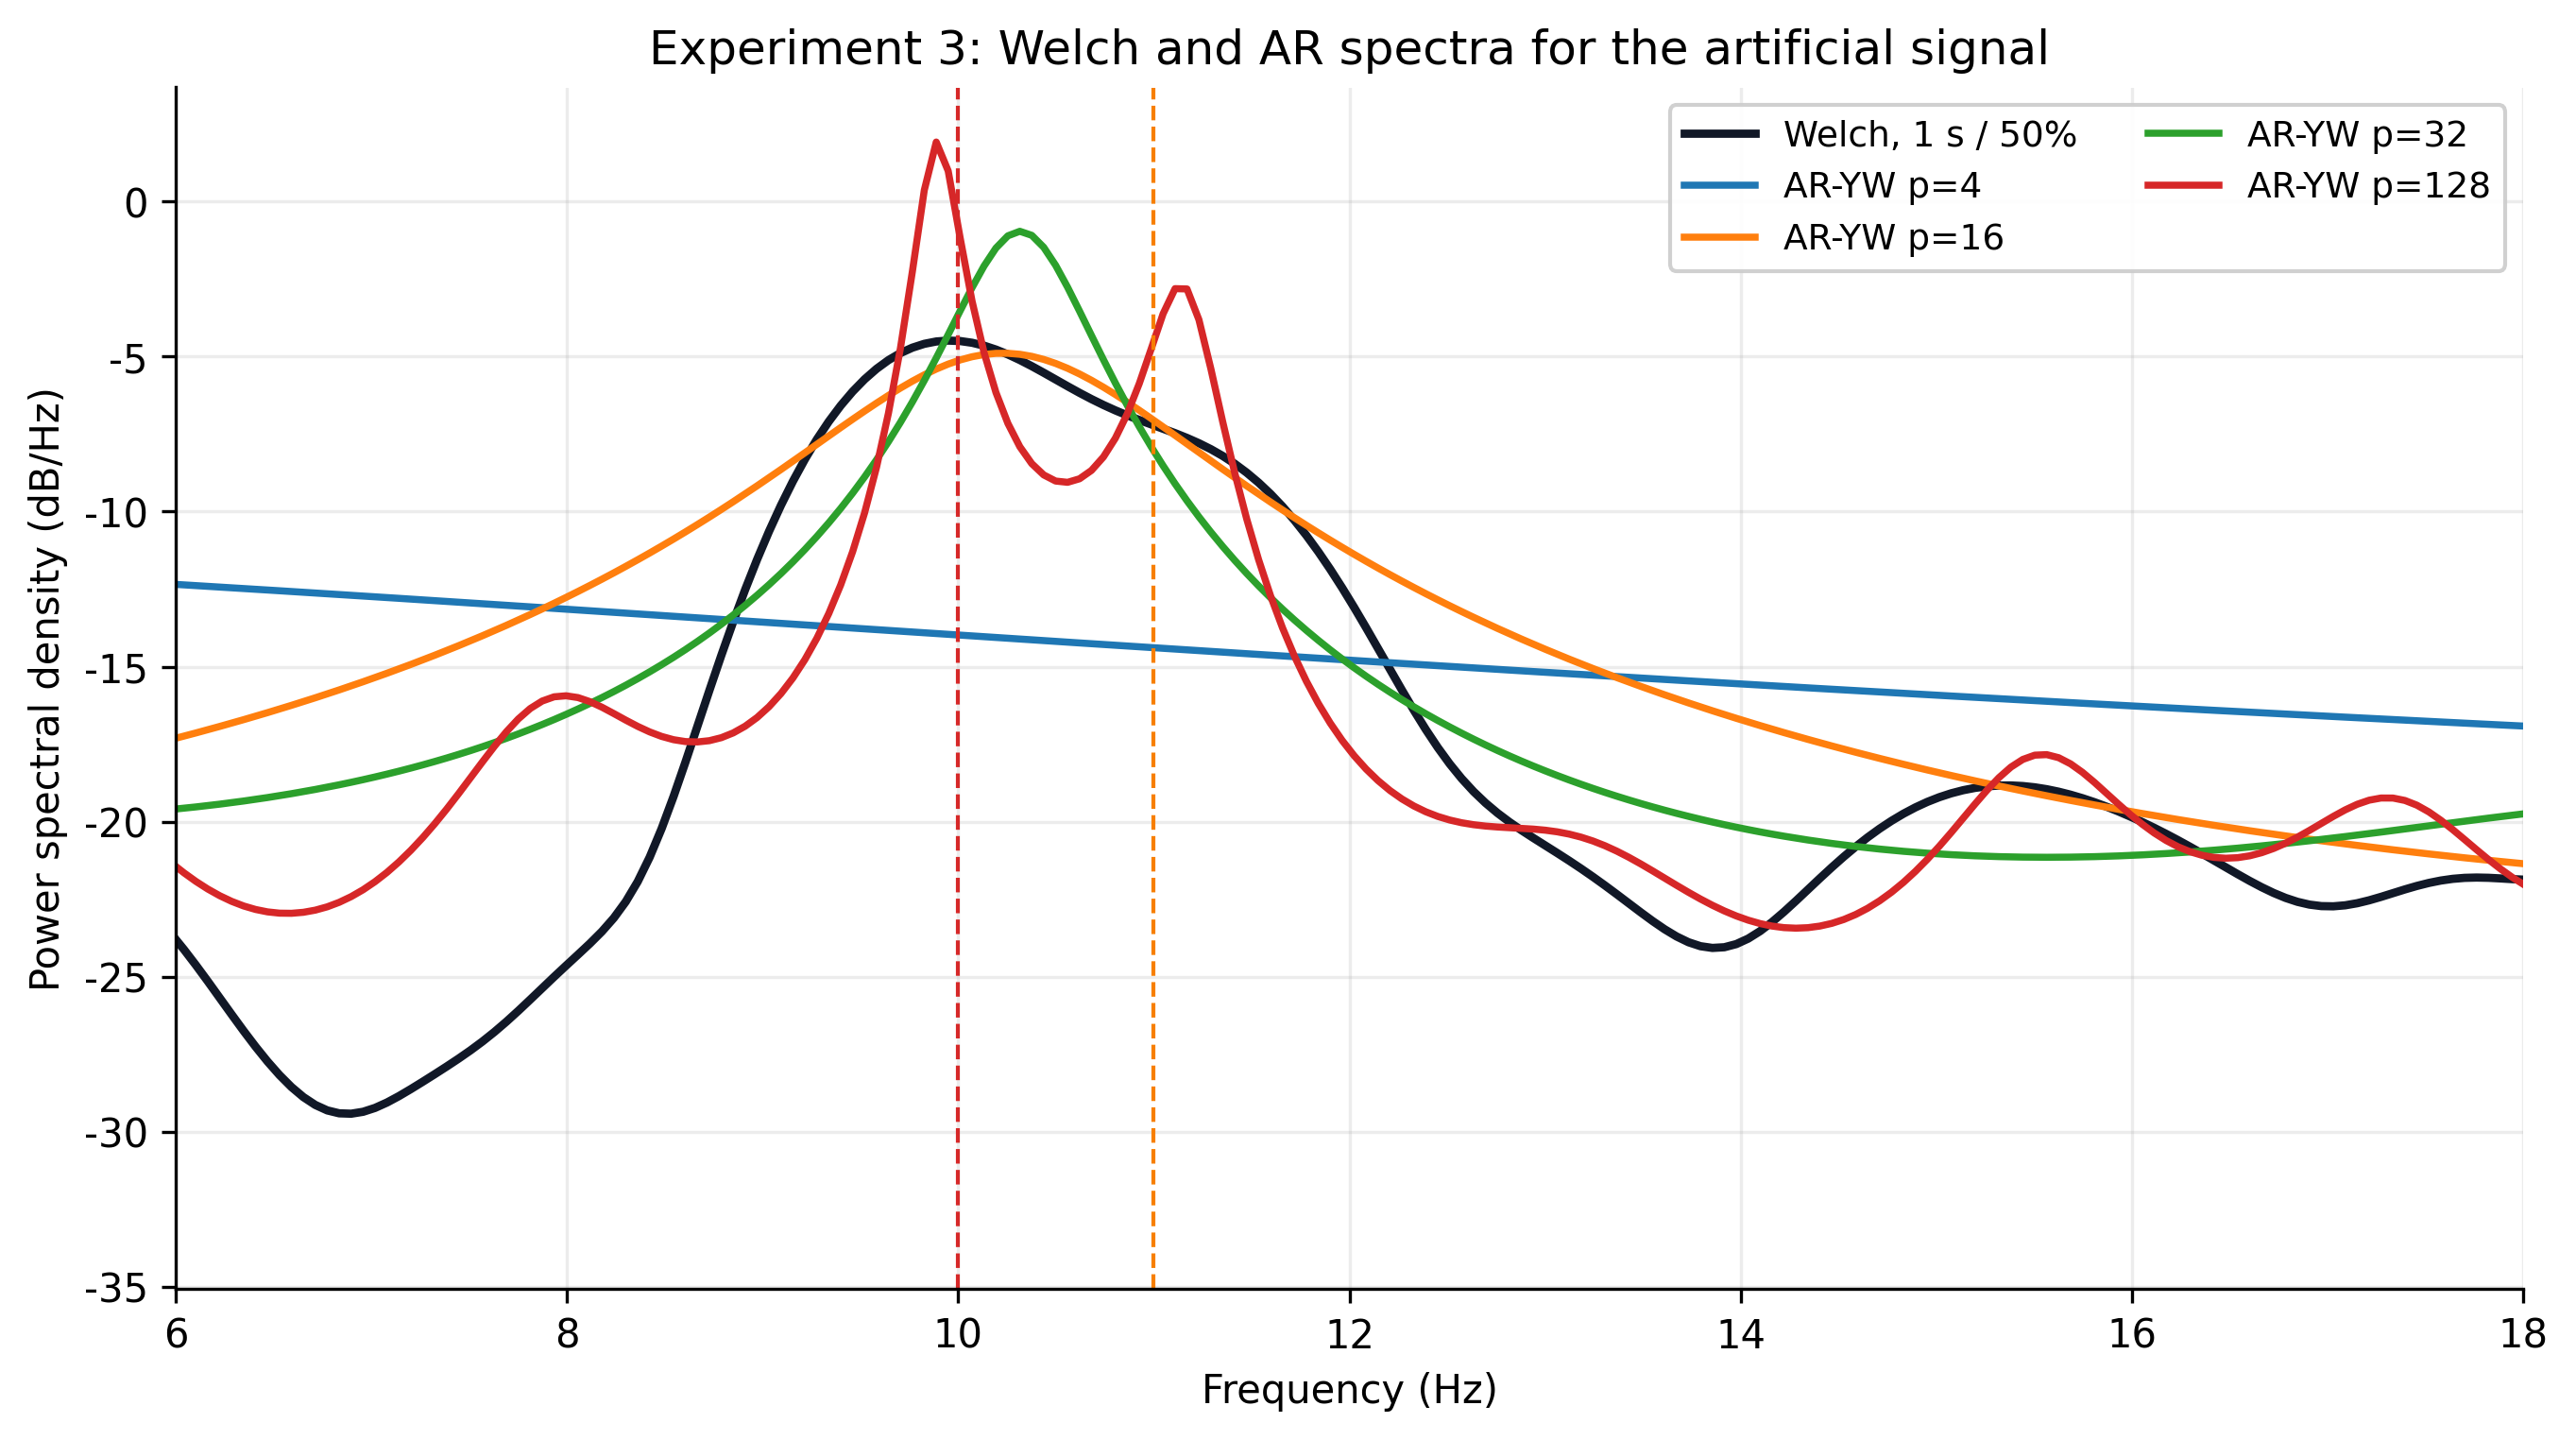
\includegraphics[width=\textwidth]{exp3_artificial_welch_ar_en.png}
\caption{Welch and representative AR spectra for the artificial signal.}
\end{figure}

\input{generated_en/table_exp3_artificial.tex}

\begin{figure}[H]
\centering
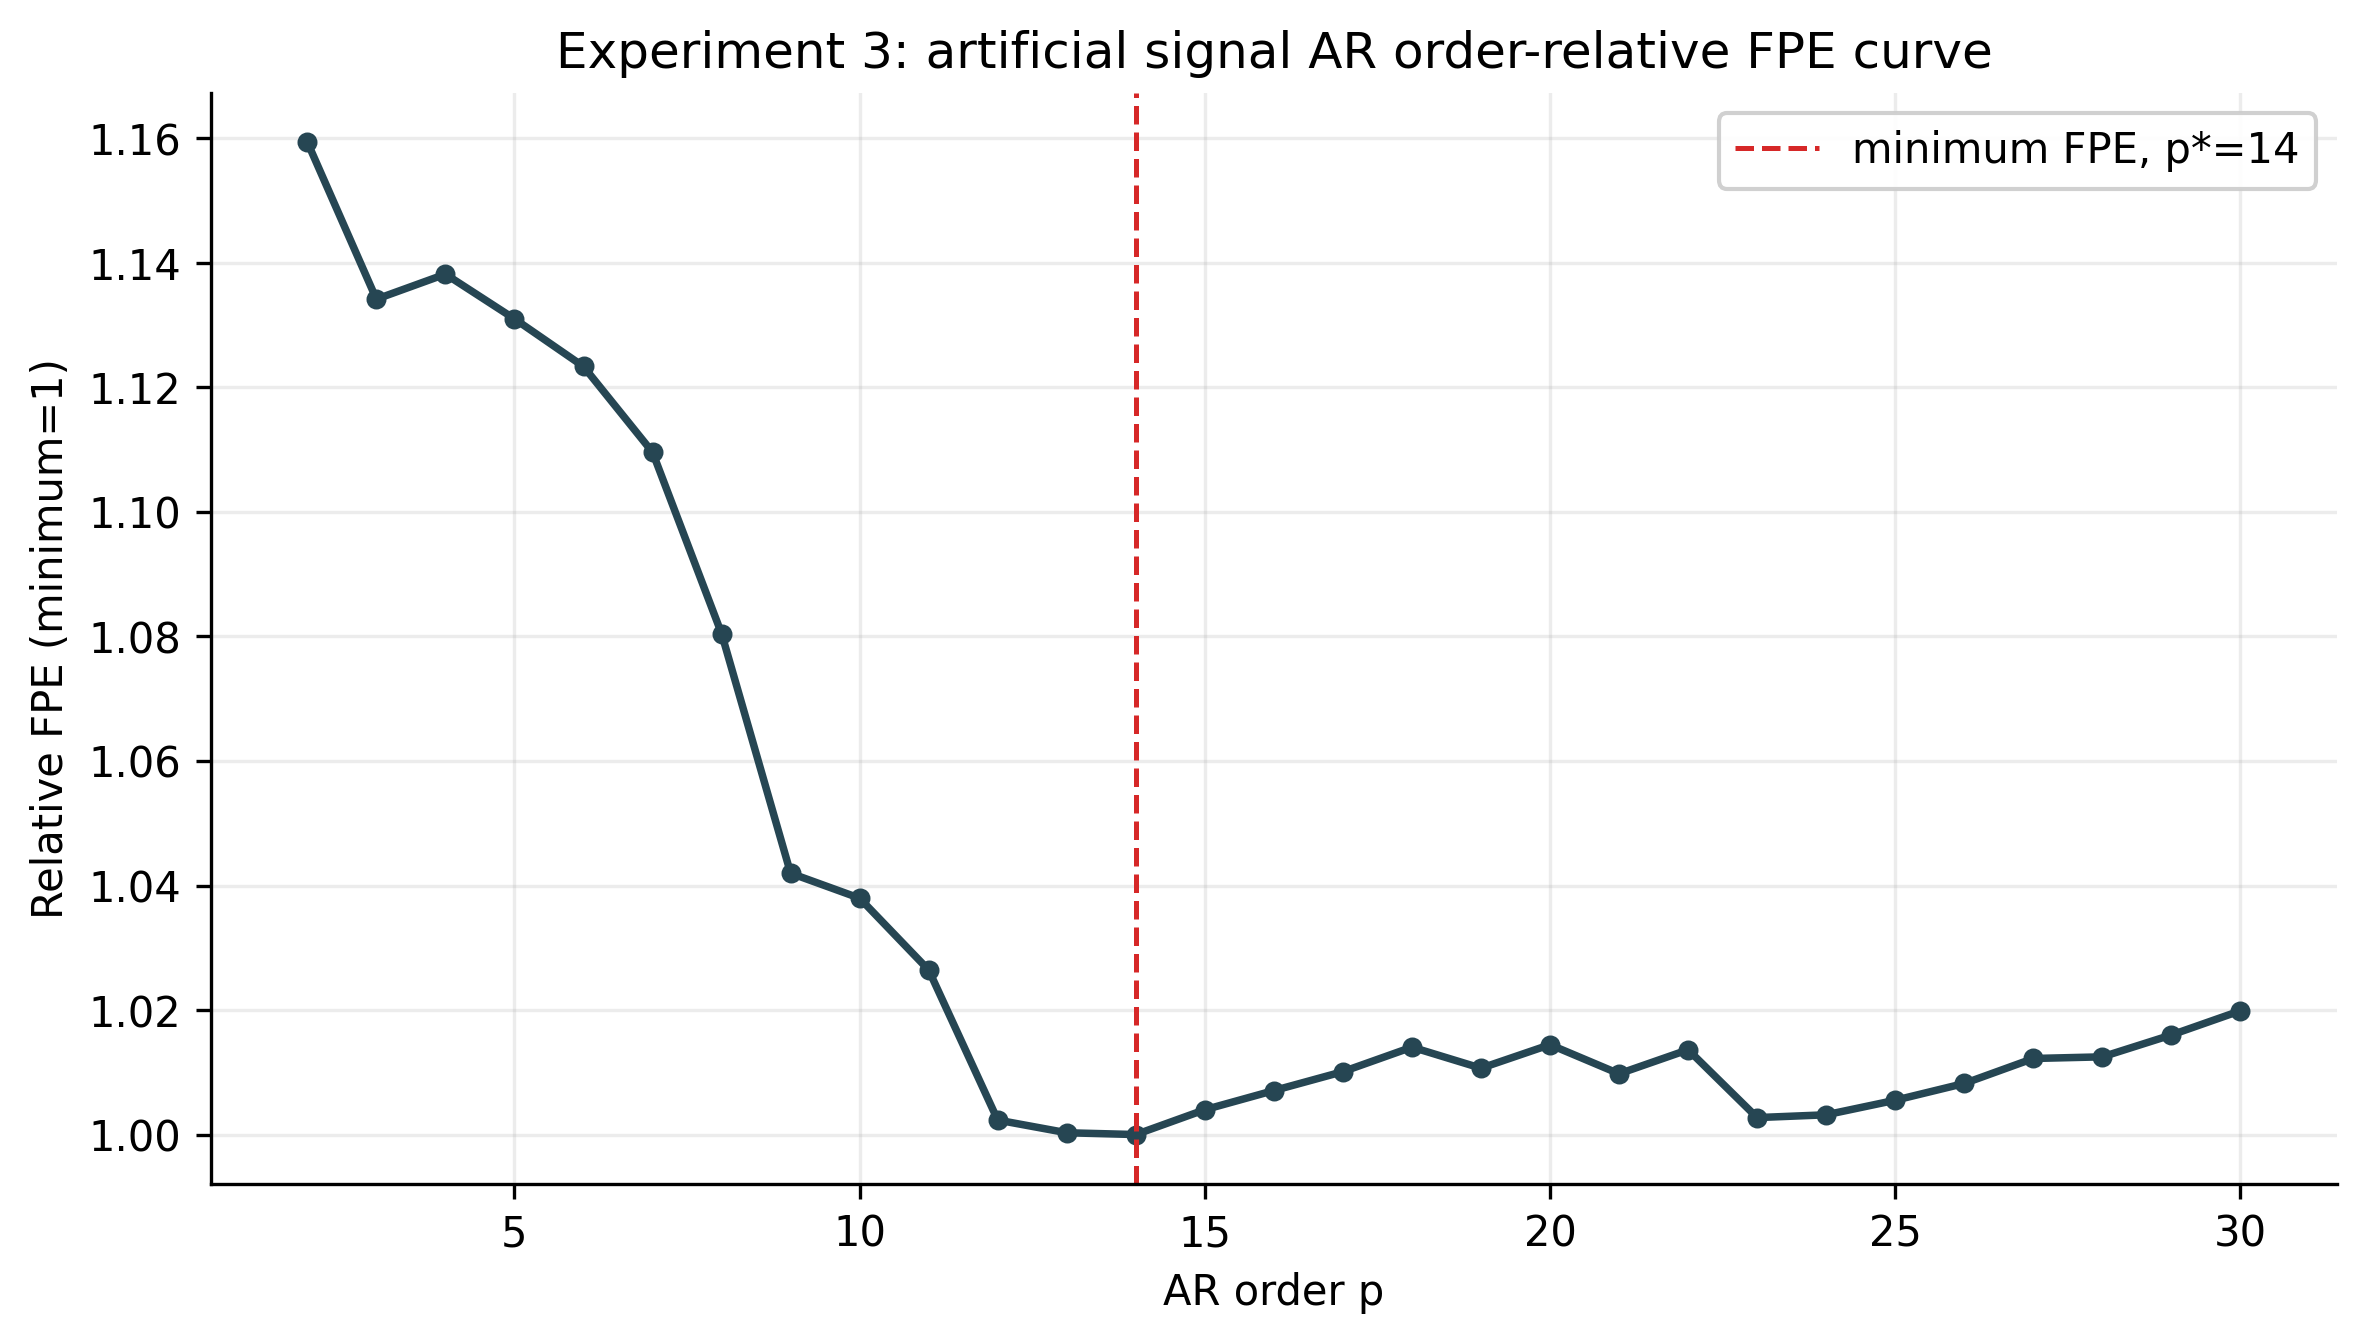
\includegraphics[width=0.86\textwidth]{exp3_artificial_fpe_en.png}
\caption{Relative FPE curve for the artificial signal, normalized by the minimum FPE.}
\end{figure}

\input{generated_en/table_exp3_artificial_fpe.tex}

\begin{figure}[H]
\centering
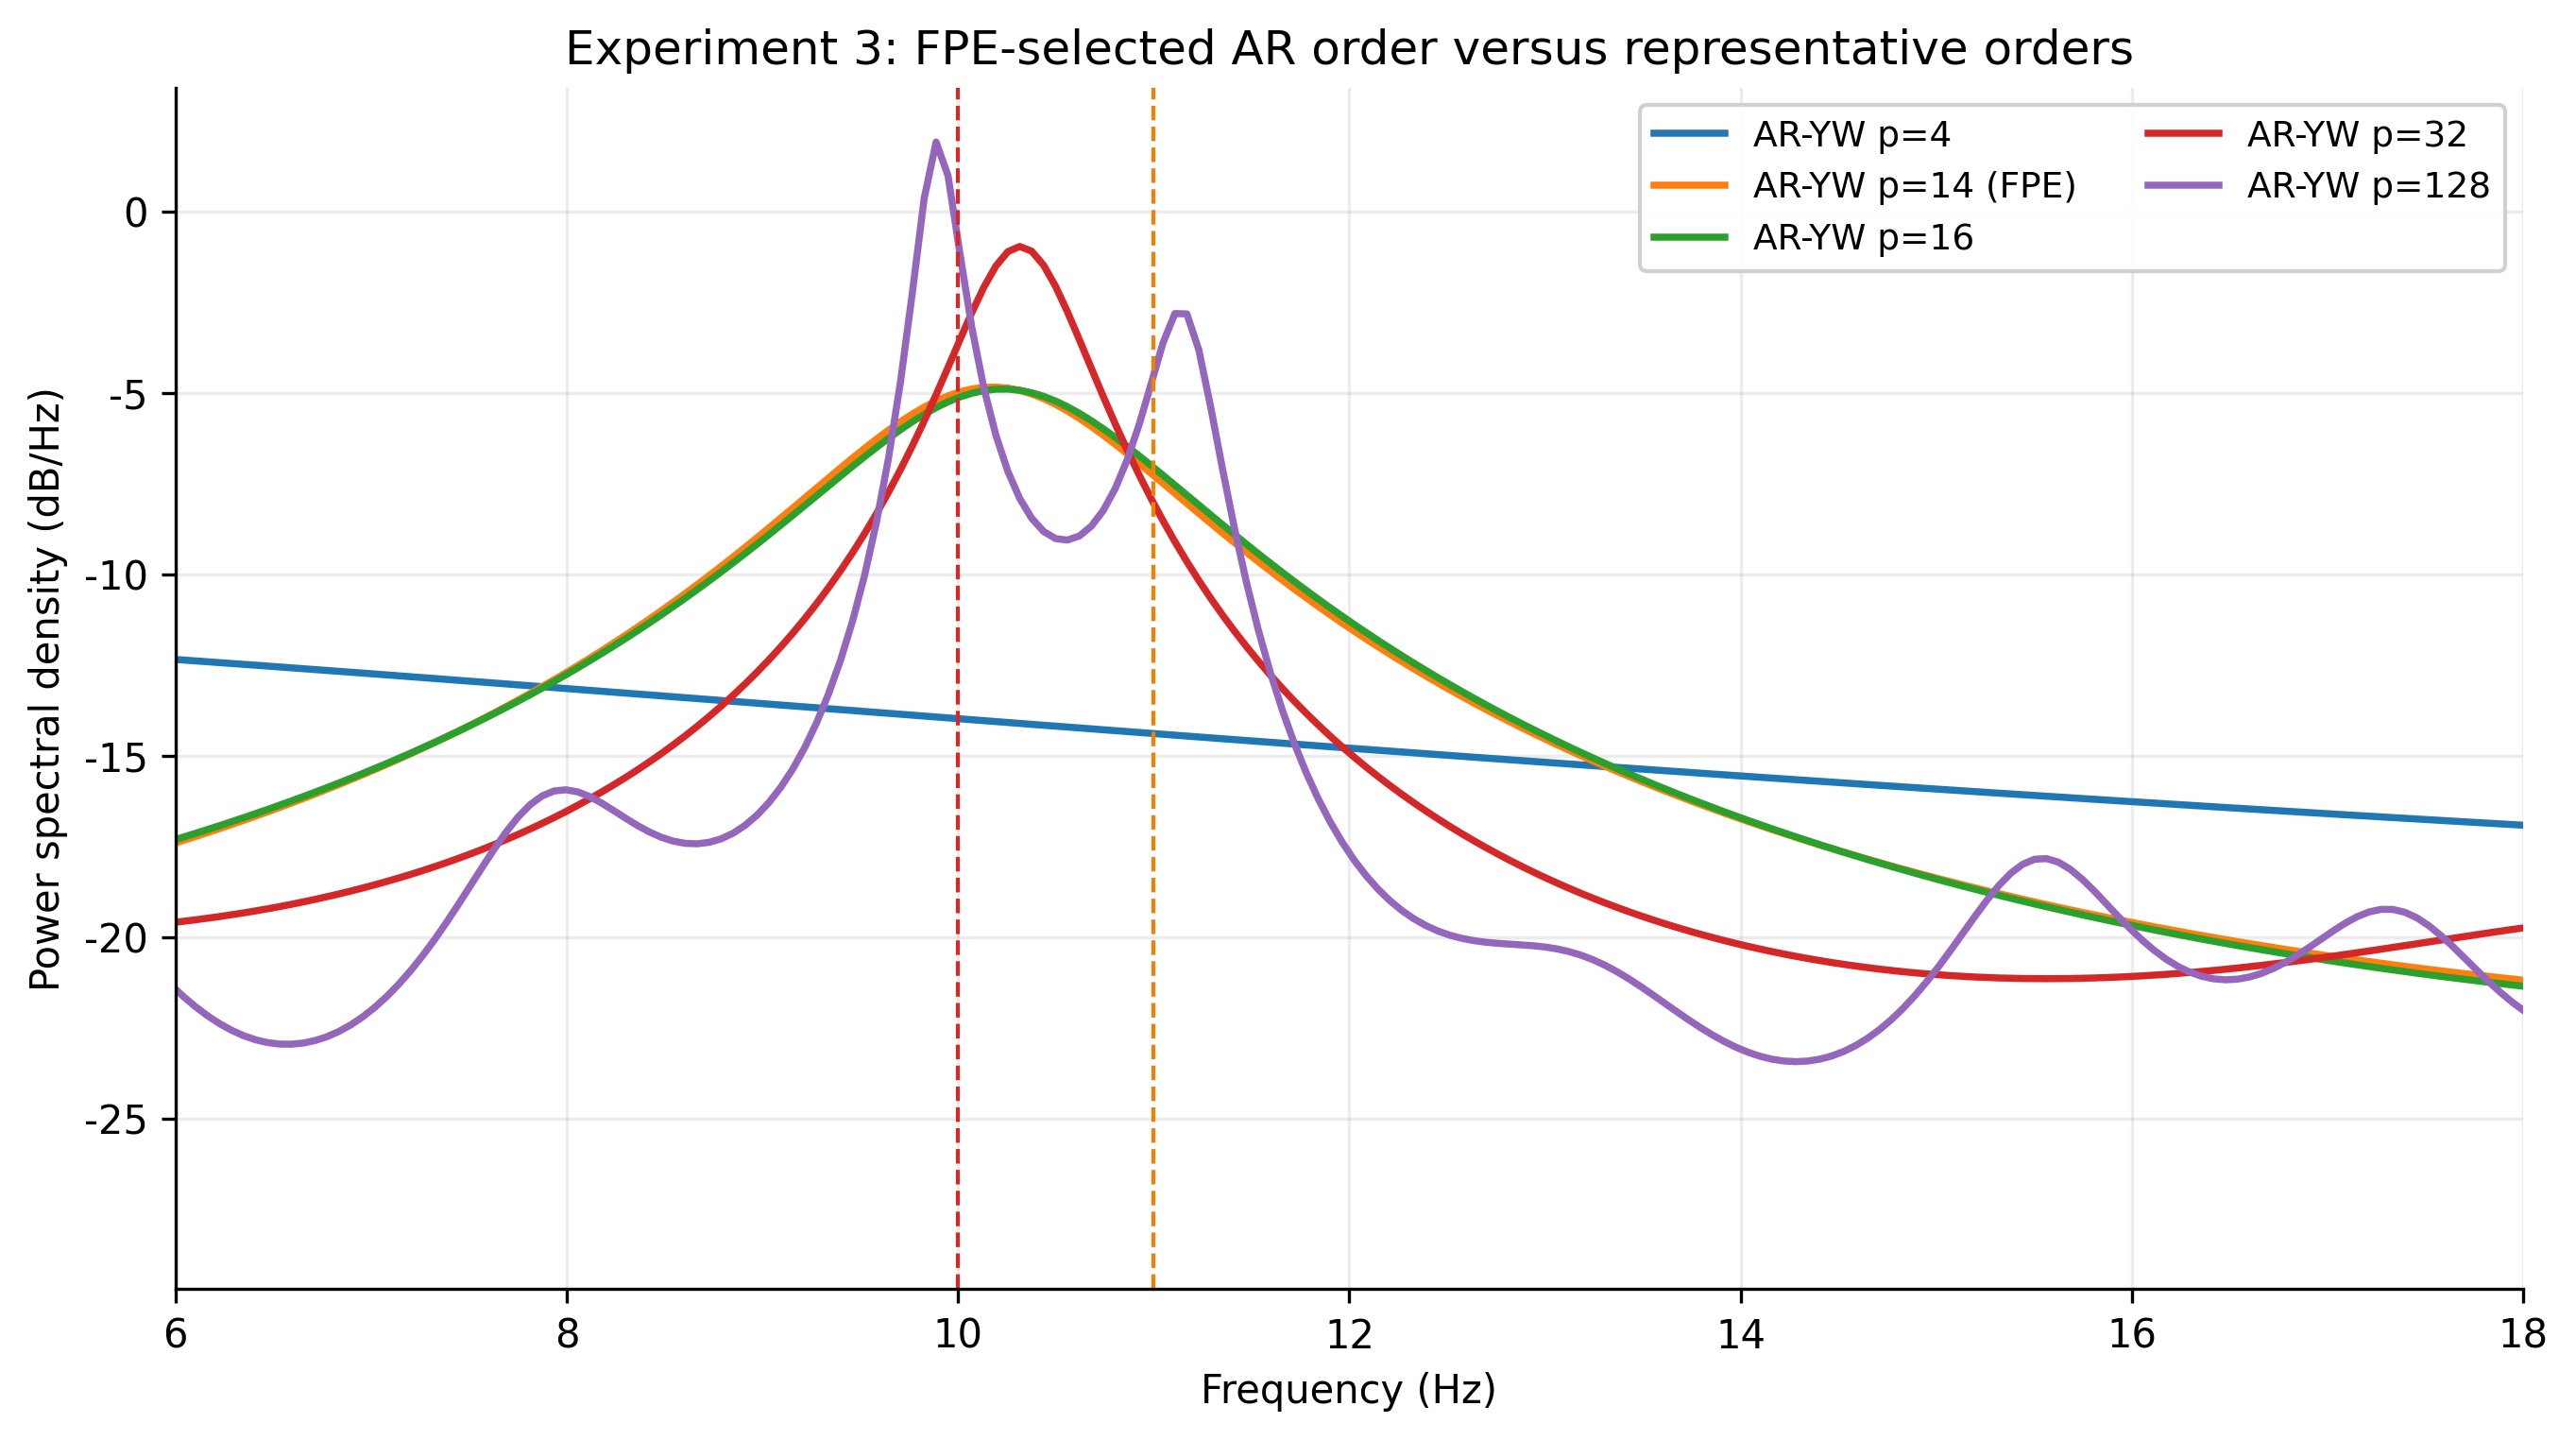
\includegraphics[width=\textwidth]{exp3_artificial_ar_pstar_en.png}
\caption{FPE-selected AR order compared with representative AR orders.}
\end{figure}

\input{generated_en/table_exp3_artificial_risk.tex}

\subsection{Real EEG}
For real EEG, the Oz segment 126.61--134.61 s is analyzed. Welch uses 2 s segments with 50\% overlap. AR spectra use representative orders $p=4,16,32,64$ and the FPE-selected order over $p=2,\ldots,80$.

\begin{figure}[H]
\centering
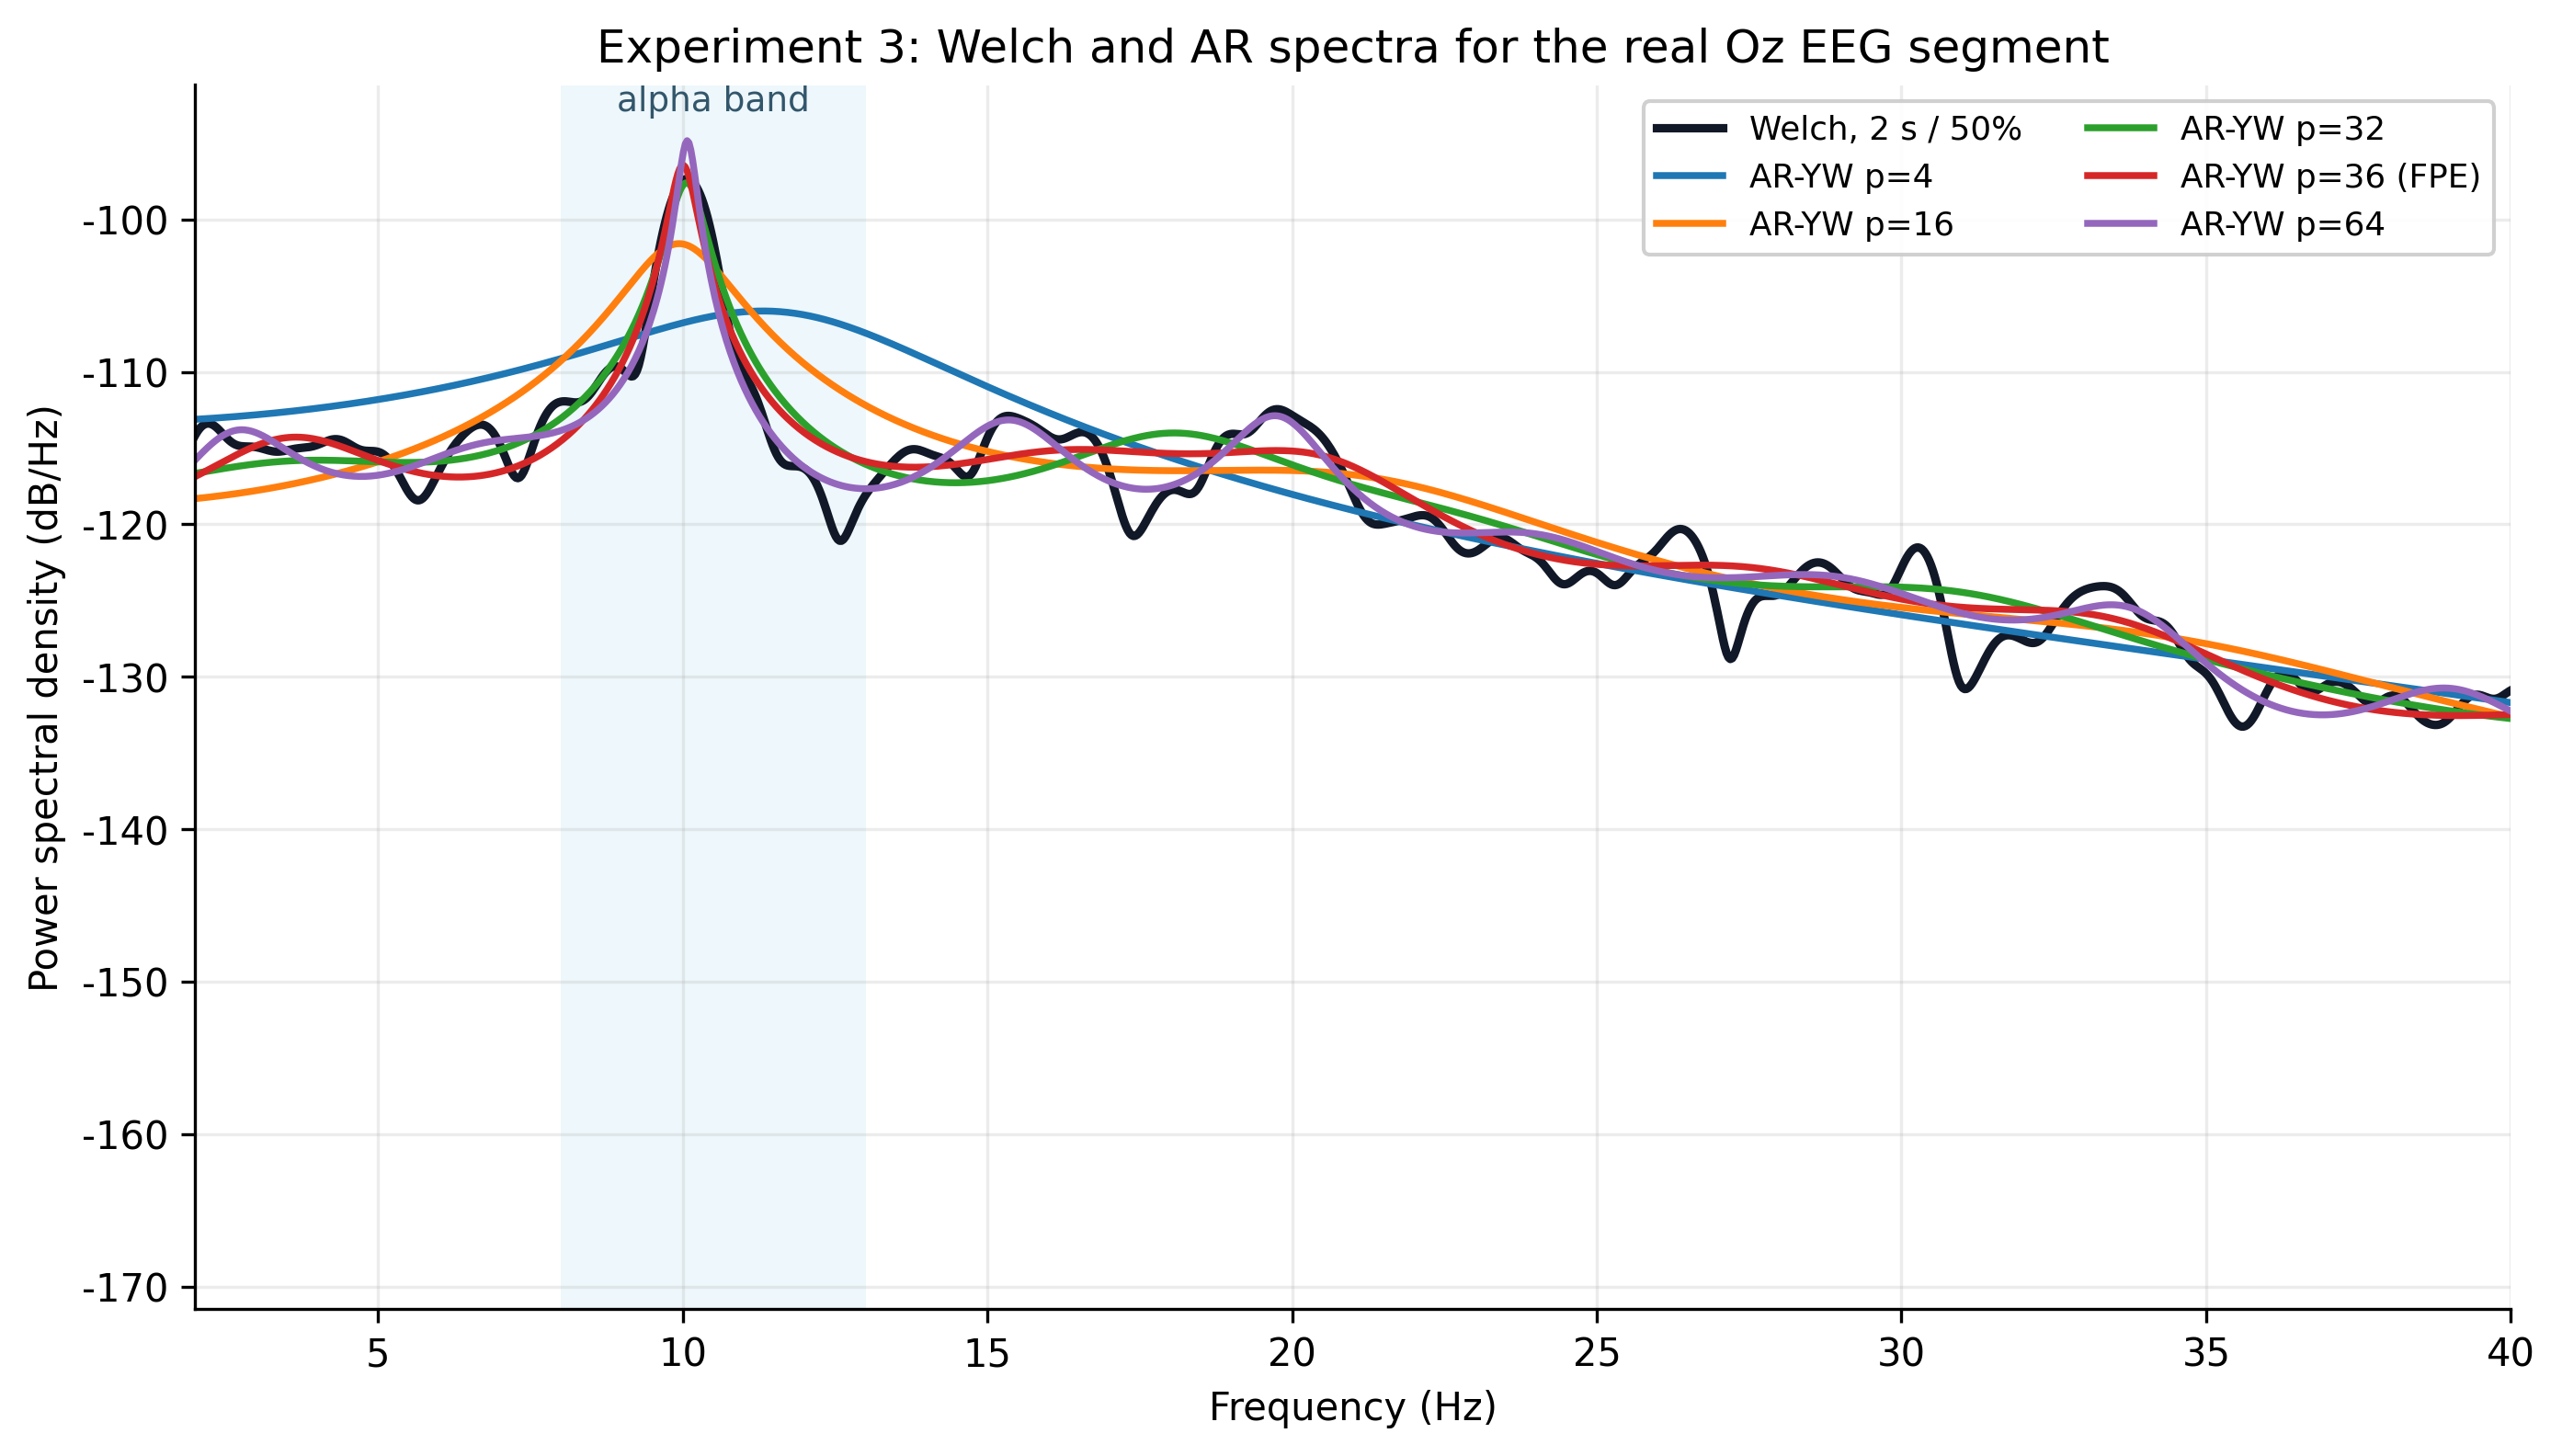
\includegraphics[width=\textwidth]{exp3_real_welch_ar_en.png}
\caption{Welch and AR spectra for the real Oz EEG segment.}
\end{figure}

\begin{figure}[H]
\centering
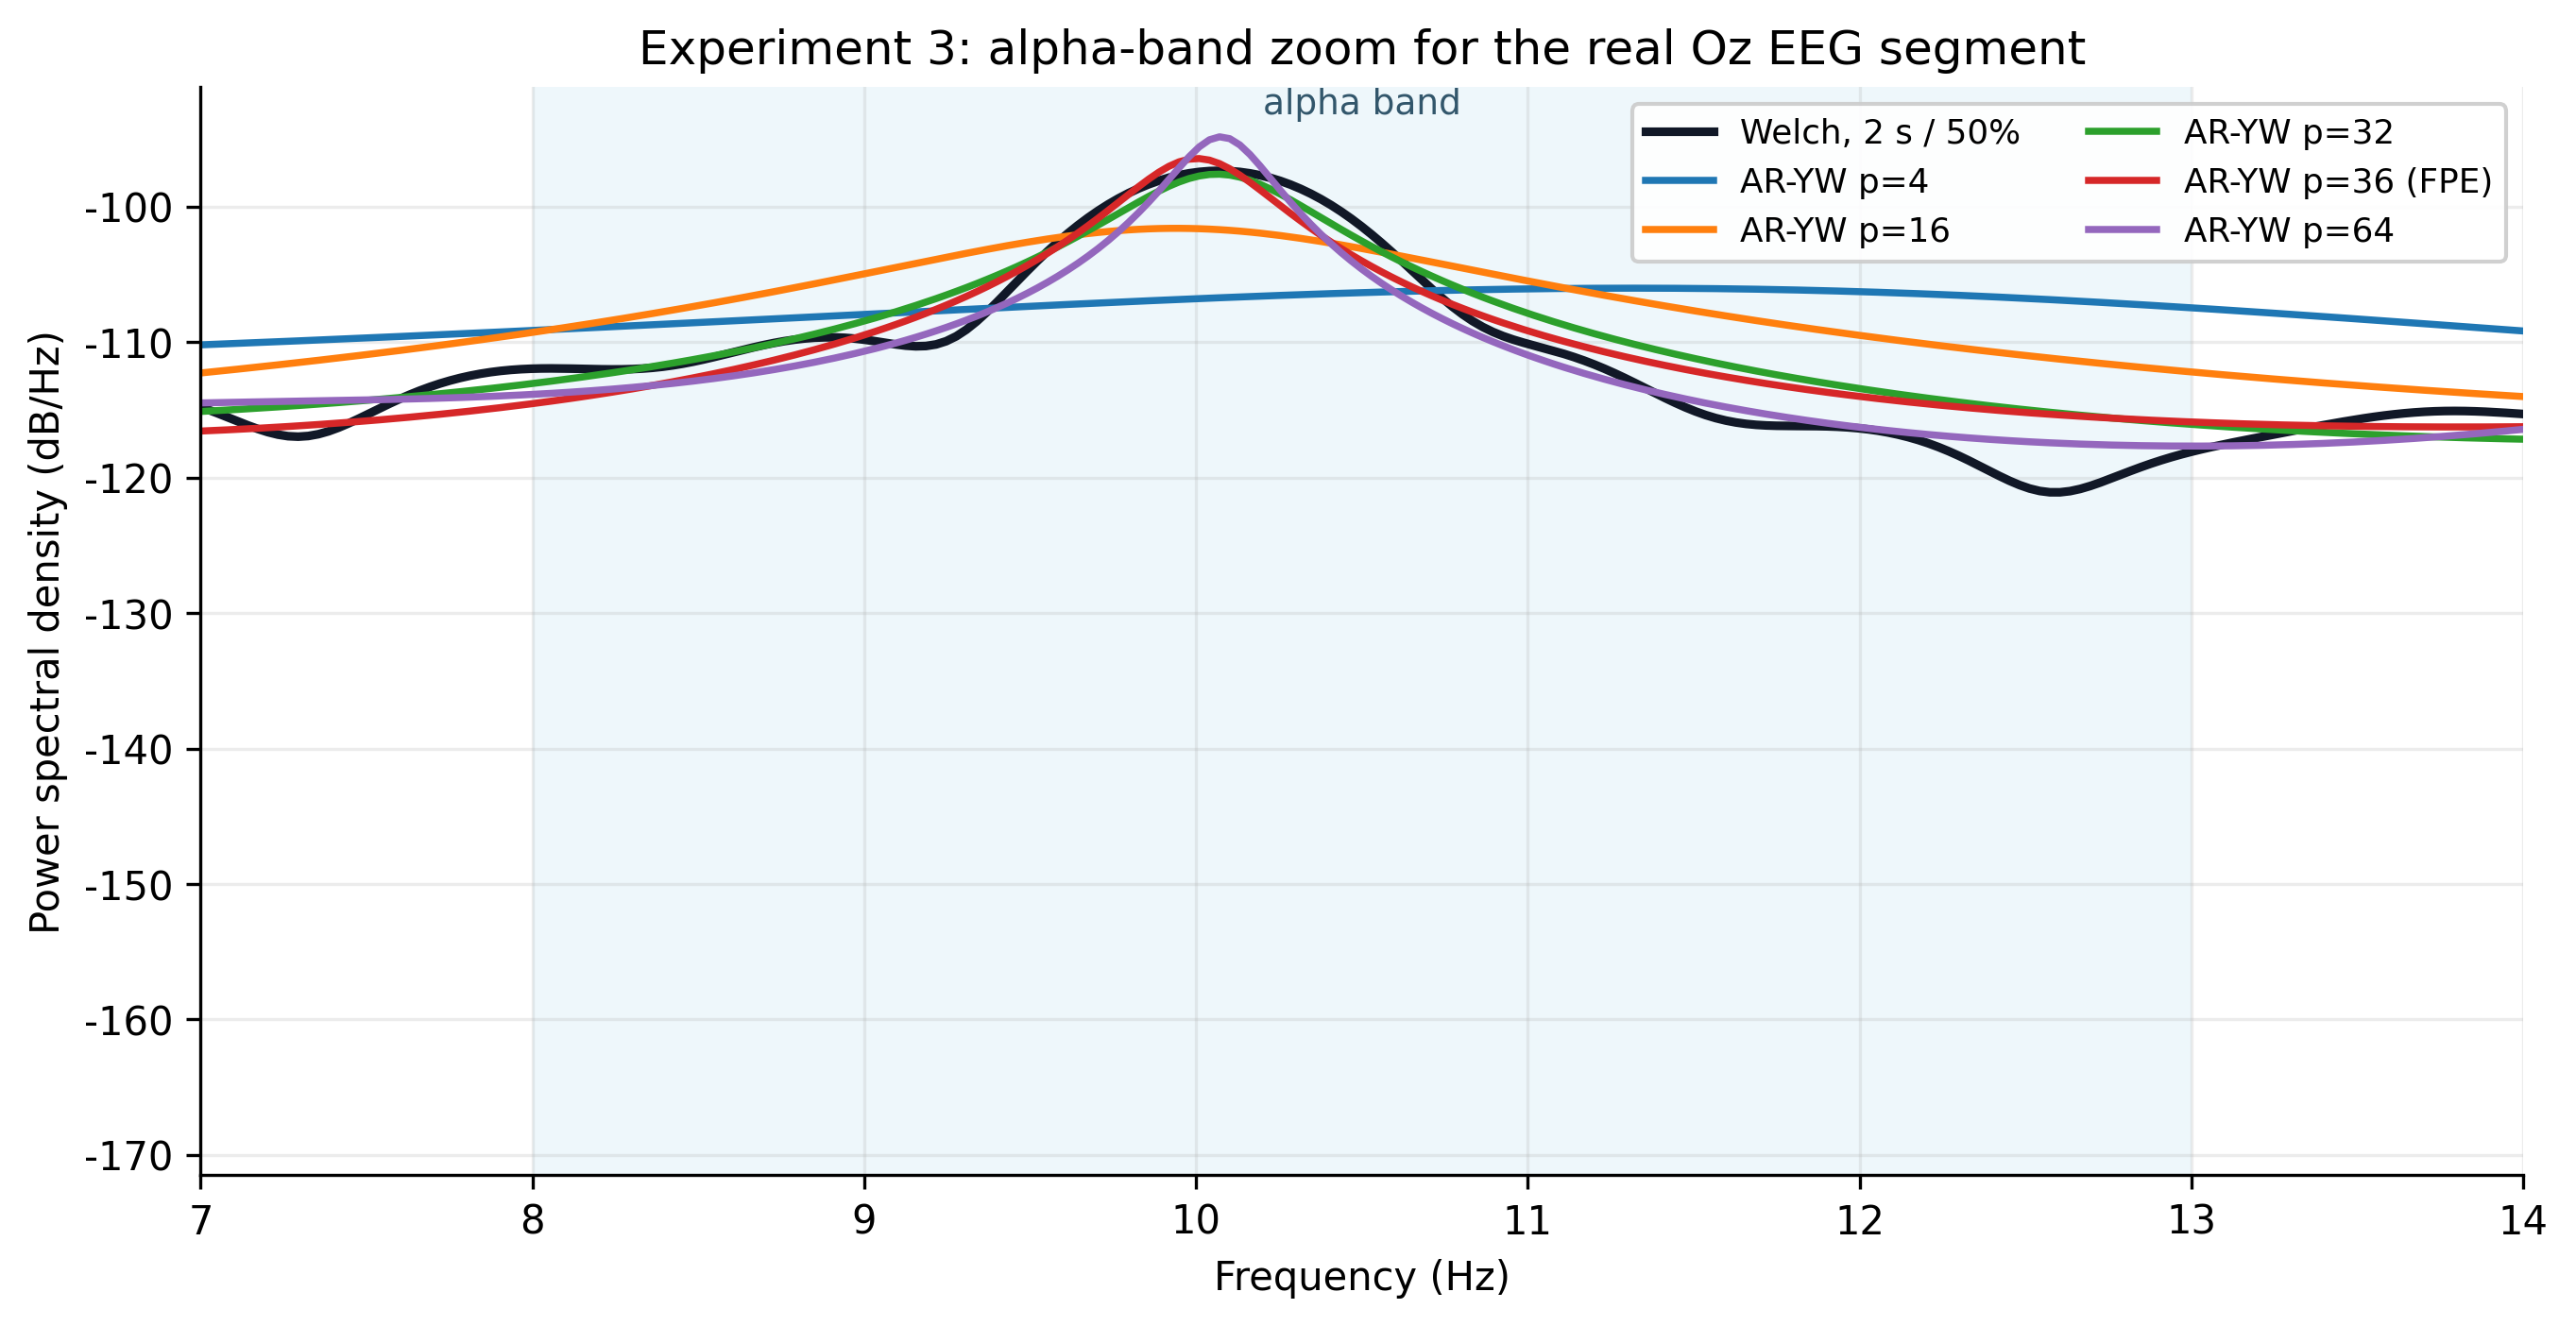
\includegraphics[width=\textwidth]{exp3_real_welch_ar_alpha_zoom_en.png}
\caption{Alpha-band zoom for the real Oz EEG segment.}
\end{figure}

\input{generated_en/table_exp3_real.tex}
\input{generated_en/table_exp3_real_risk.tex}

\begin{figure}[H]
\centering
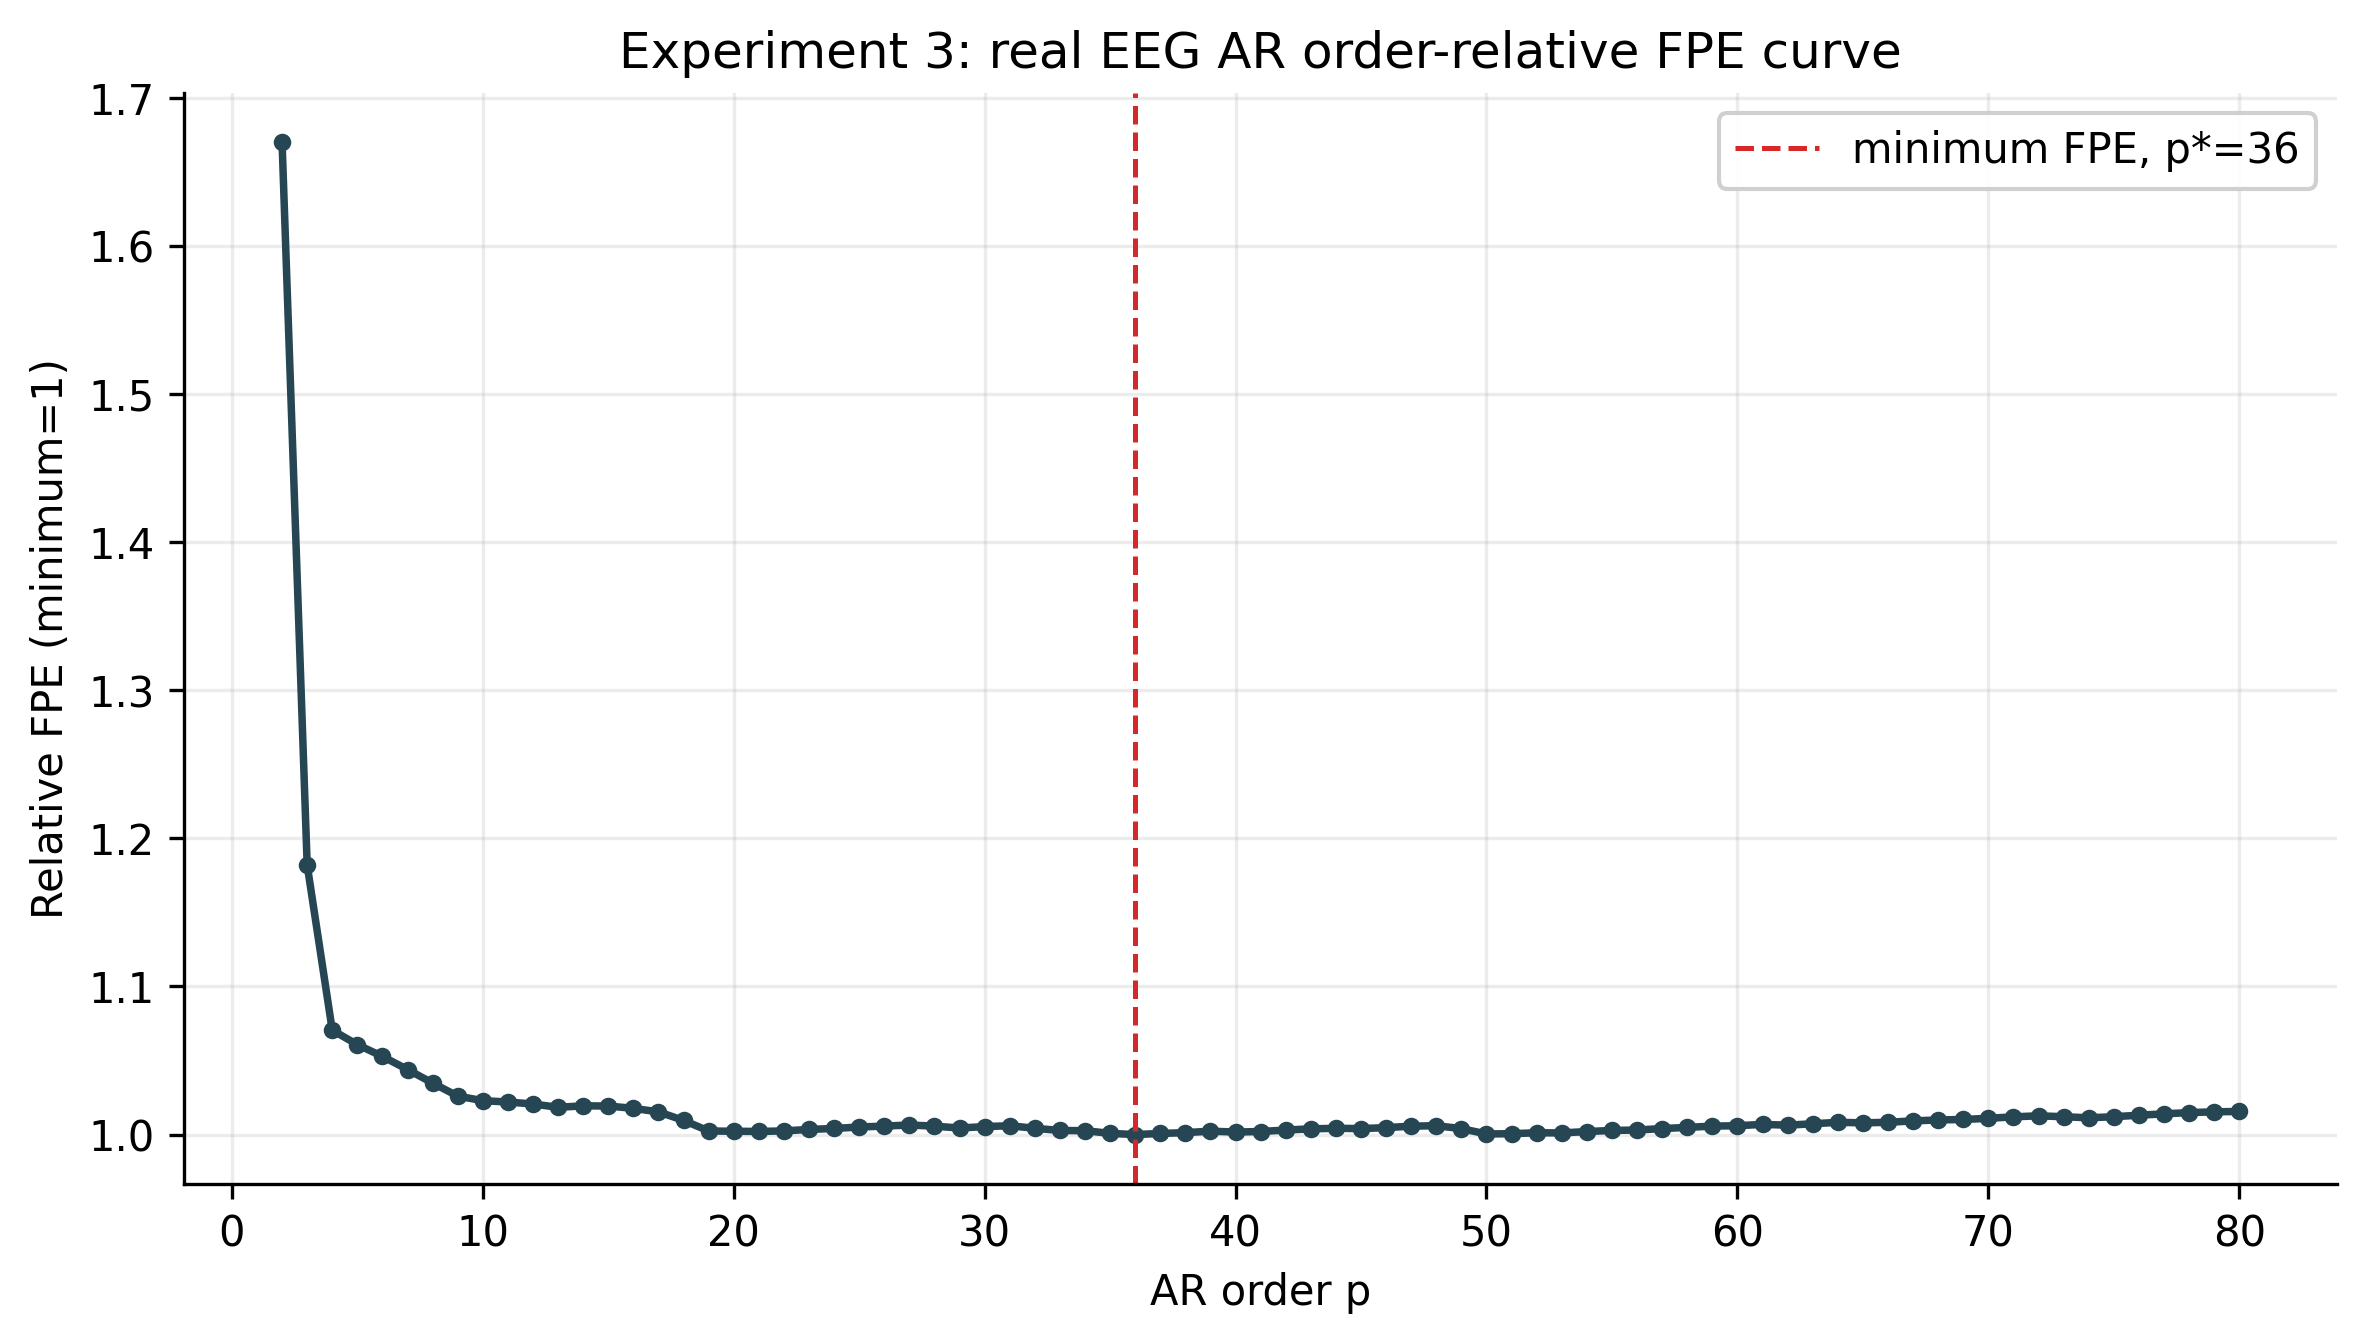
\includegraphics[width=0.86\textwidth]{exp3_real_fpe_en.png}
\caption{Relative FPE curve for the real EEG segment, normalized by the minimum FPE.}
\end{figure}

\input{generated_en/table_exp3_real_fpe.tex}

\subsection{Discussion}
AR spectra can look sharper than Welch spectra on short data because the fitted autoregressive model extrapolates a parametric spectral shape rather than averaging noisy periodograms. Low AR orders oversmooth and merge close components. High orders can split peaks and create pseudo-peaks. FPE minimizes a prediction-error criterion, but the visually or physiologically most credible spectrum still needs context from bandwidth, peak stability, and background behavior.

\textbf{Question: Why is a sharper AR alpha peak not automatically more physiological?}
Answer: Sharpness can come from model order and pole placement rather than neural rhythm. In real EEG, very narrow peaks and extra local peaks can be artifacts of overfitting.

\section{Experiment 4: Periodogram Instability and Welch Averaging}

\subsection{Same Random Process, Multiple Realizations}
Thirty independent 8 s signals are generated as $\sin(2\pi10t)+w_k(t)$. Each realization is analyzed by an 8 s Hamming periodogram and by Welch with 2 s segments, 50\% overlap, and a Hamming window.

\begin{figure}[H]
\centering
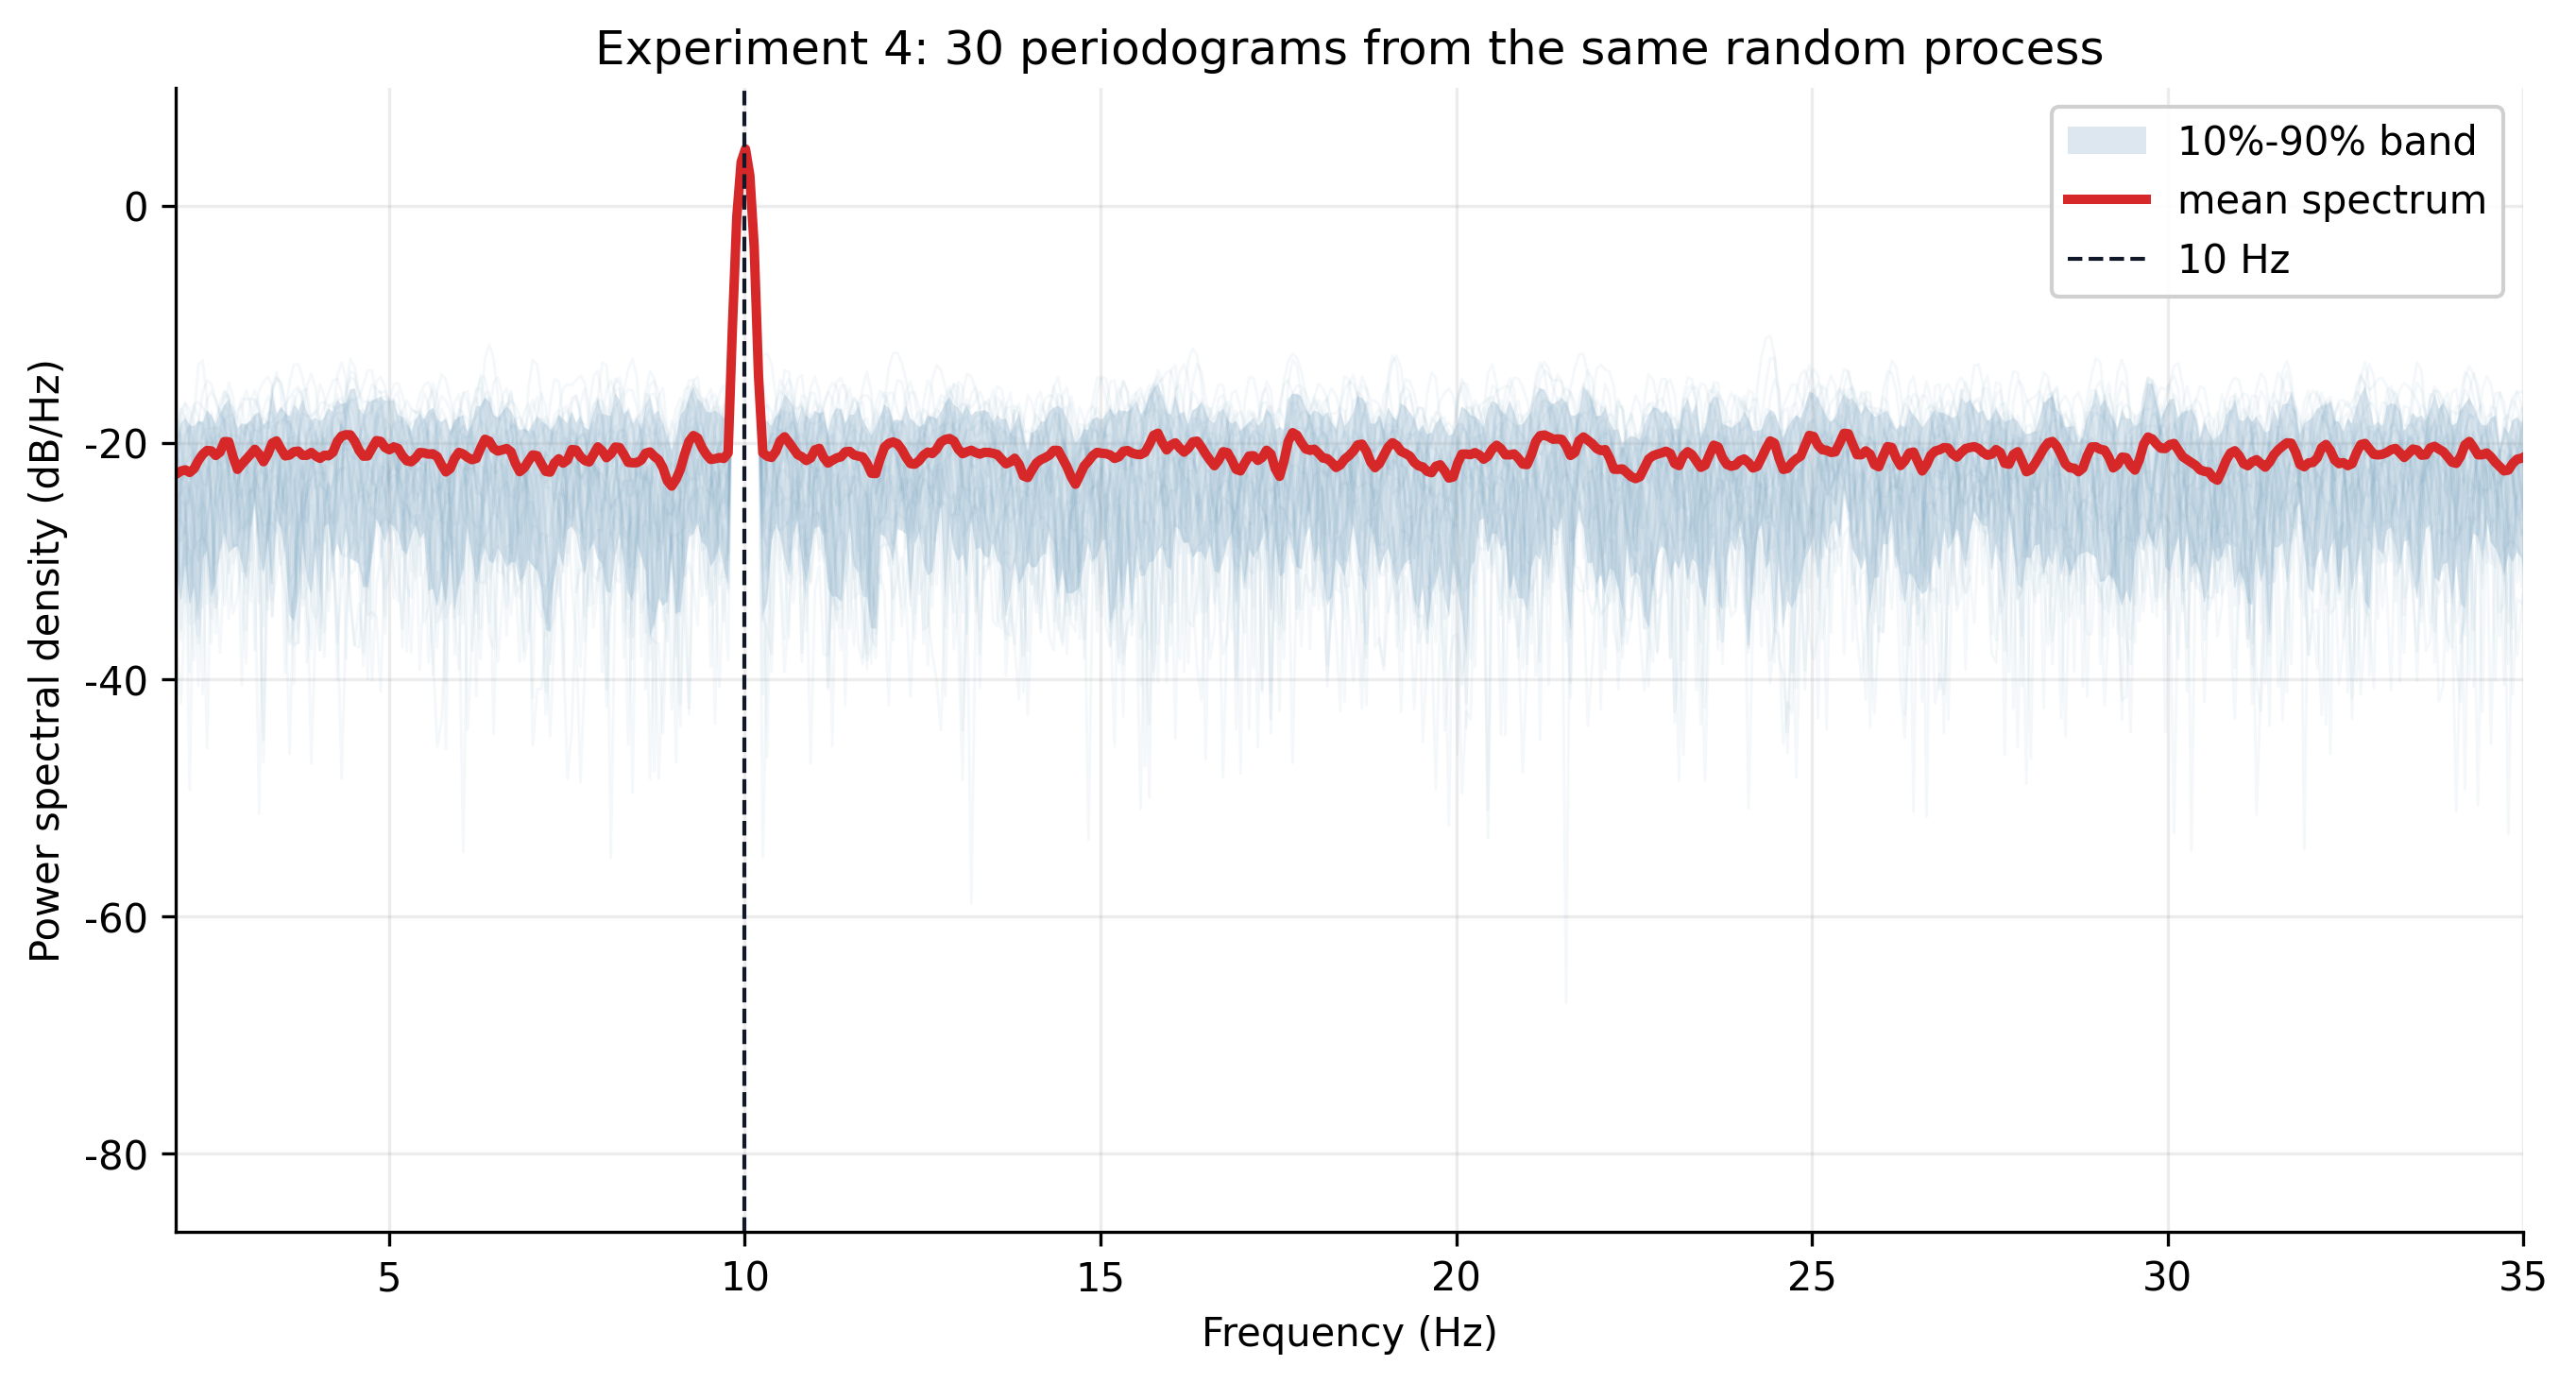
\includegraphics[width=\textwidth]{exp4_artificial_periodogram_30_en.png}
\caption{Thirty single periodograms from the same random process.}
\end{figure}

\begin{figure}[H]
\centering
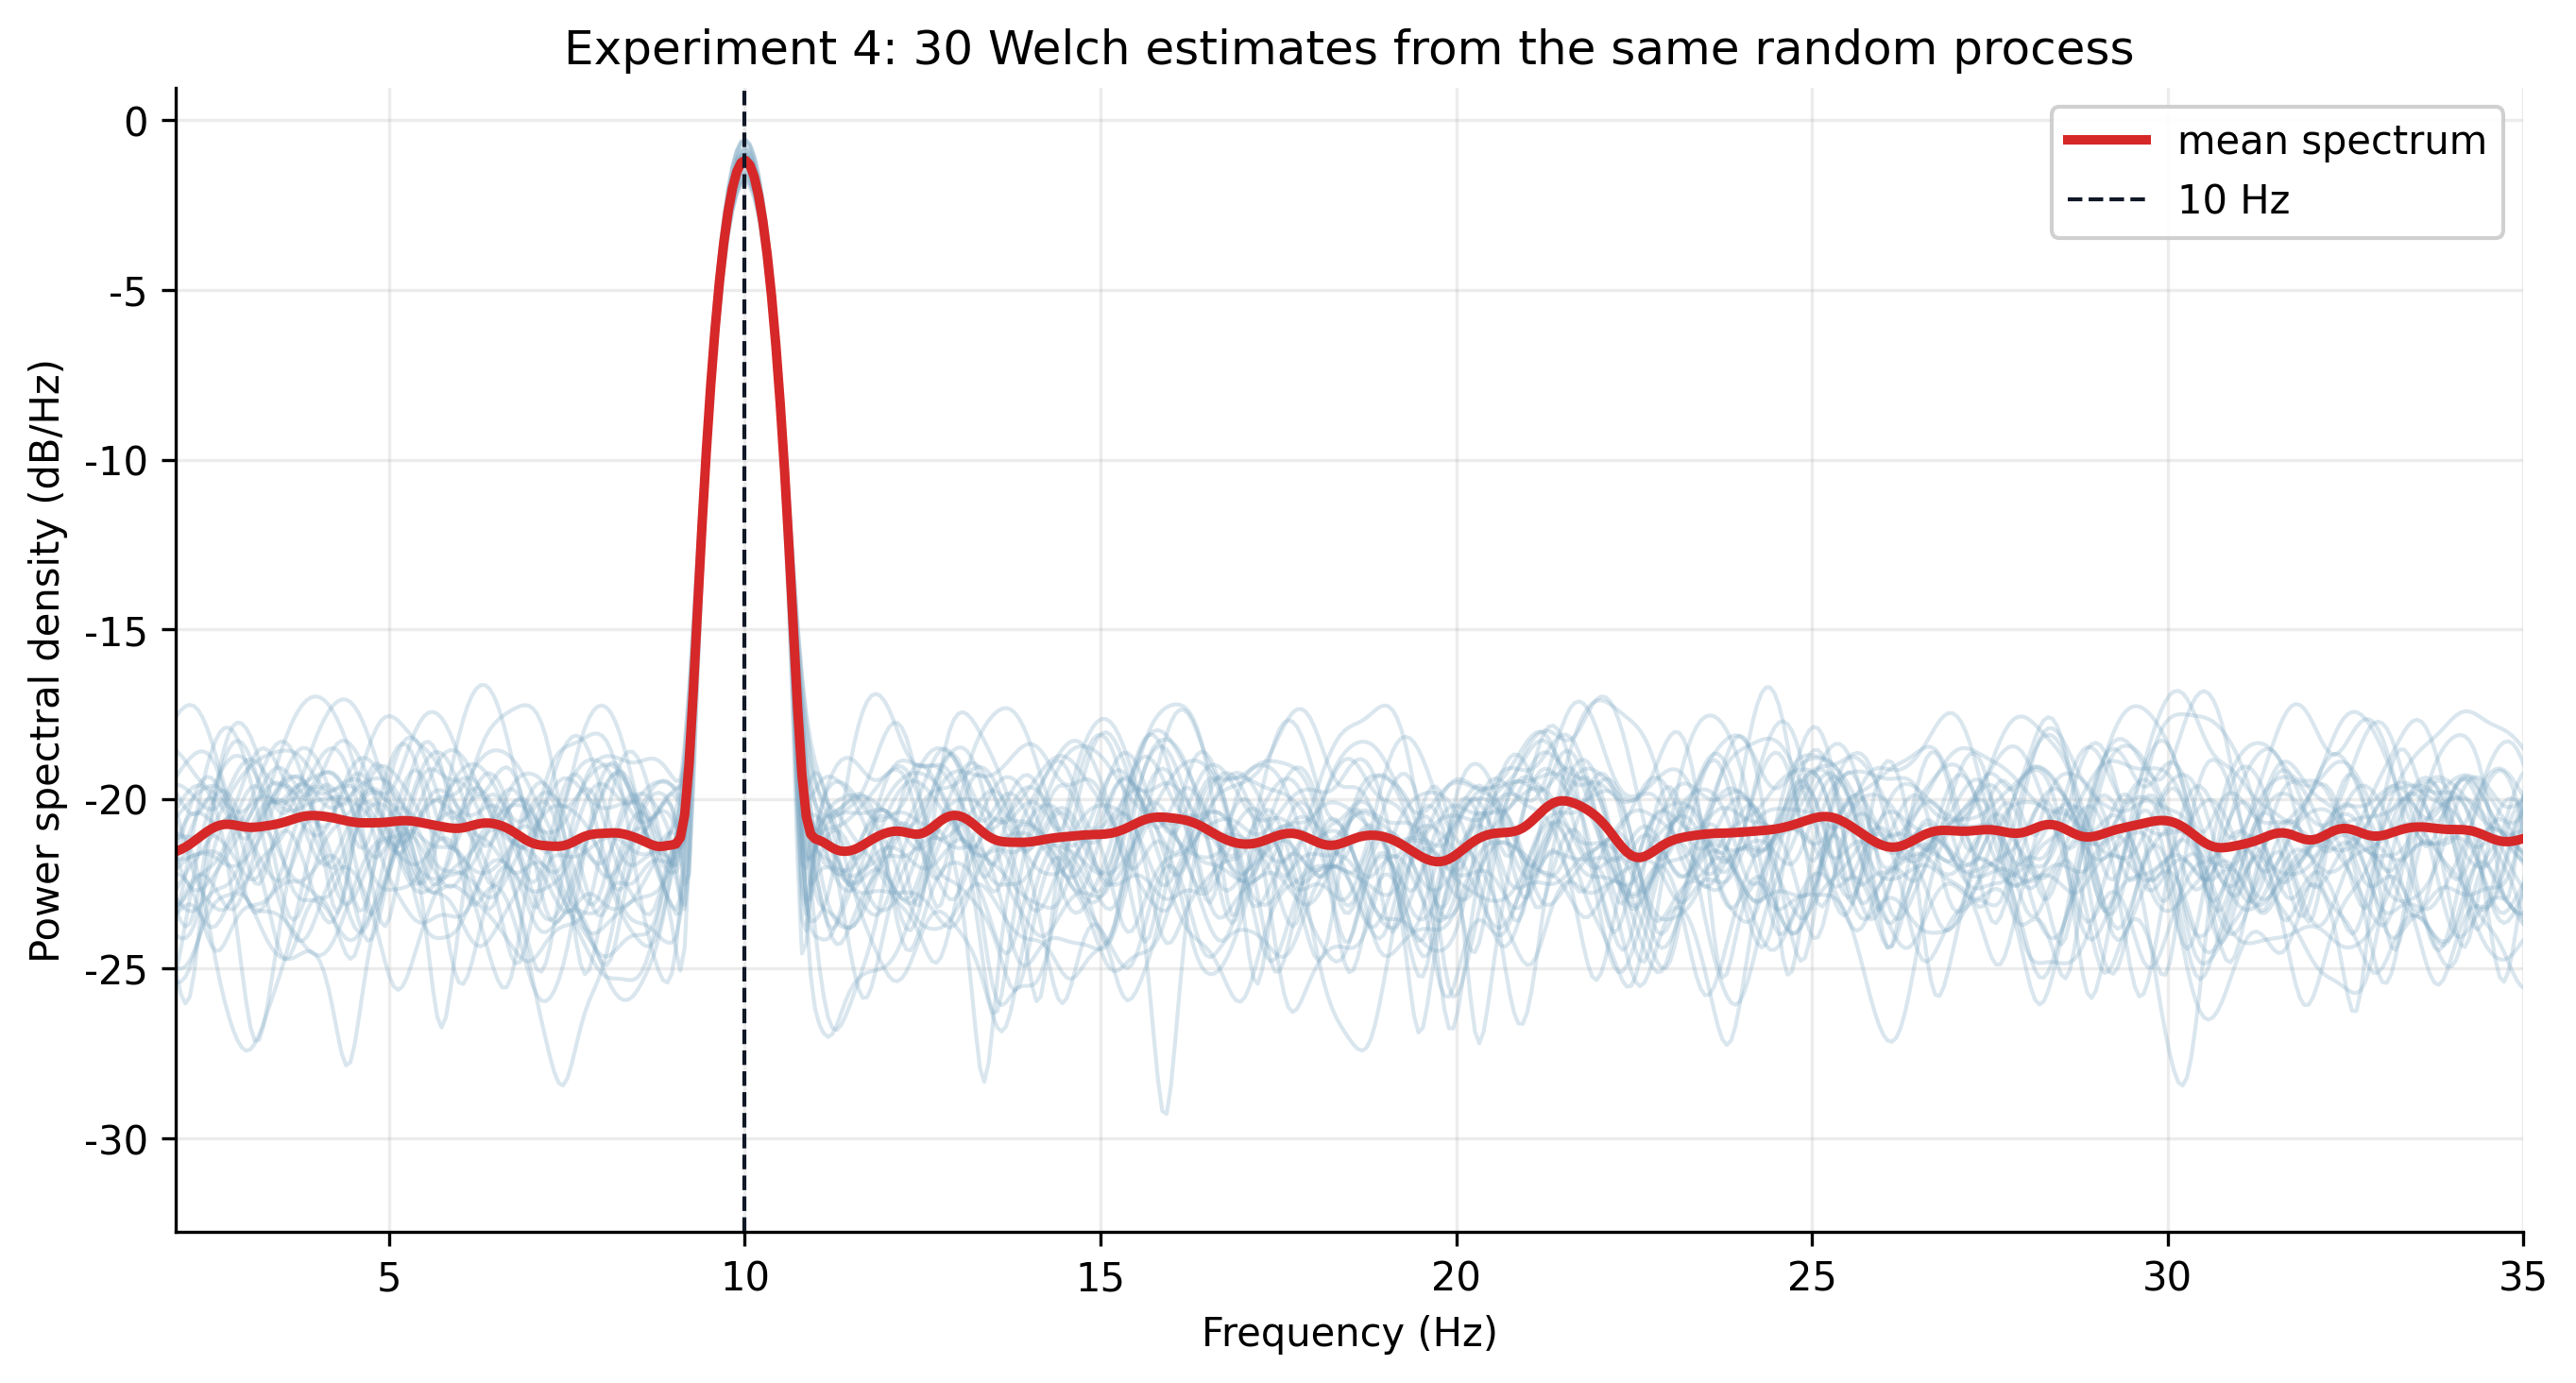
\includegraphics[width=\textwidth]{exp4_artificial_welch_30_en.png}
\caption{Thirty Welch spectra from the same random process.}
\end{figure}

\begin{figure}[H]
\centering
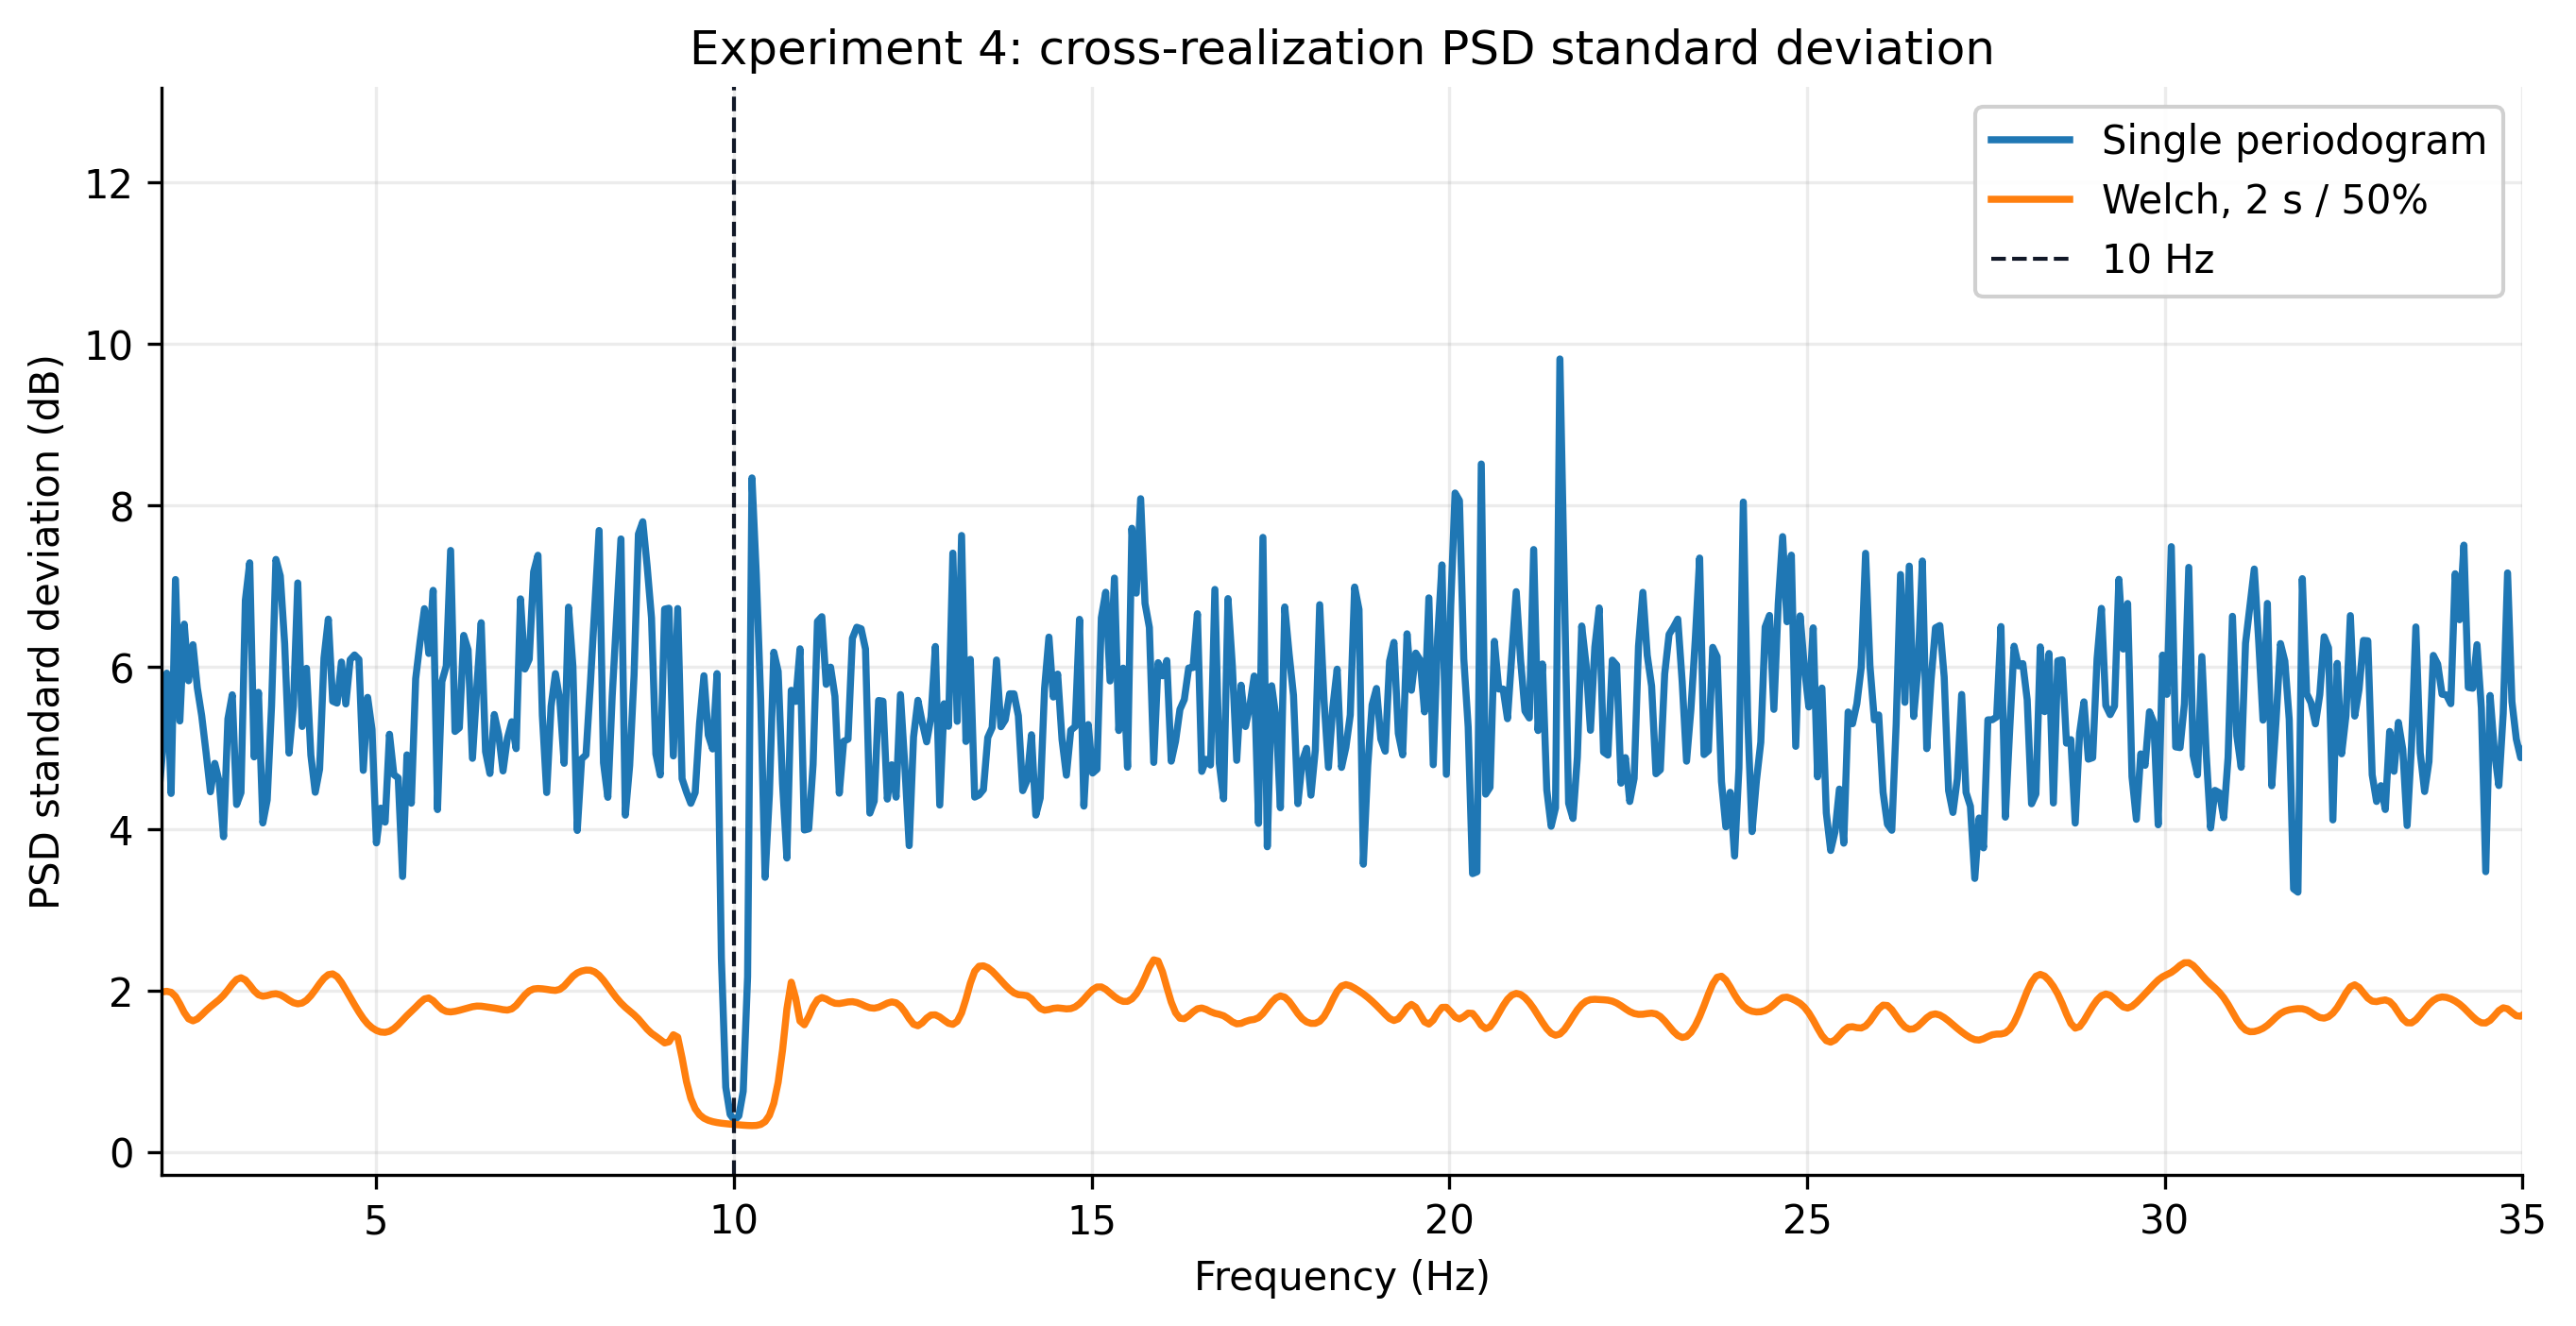
\includegraphics[width=\textwidth]{exp4_artificial_std_comparison_en.png}
\caption{Cross-realization pointwise PSD standard deviation.}
\end{figure}

\input{generated_en/table_exp4_realizations.tex}

\subsection{Welch Segment Length}
\begin{figure}[H]
\centering
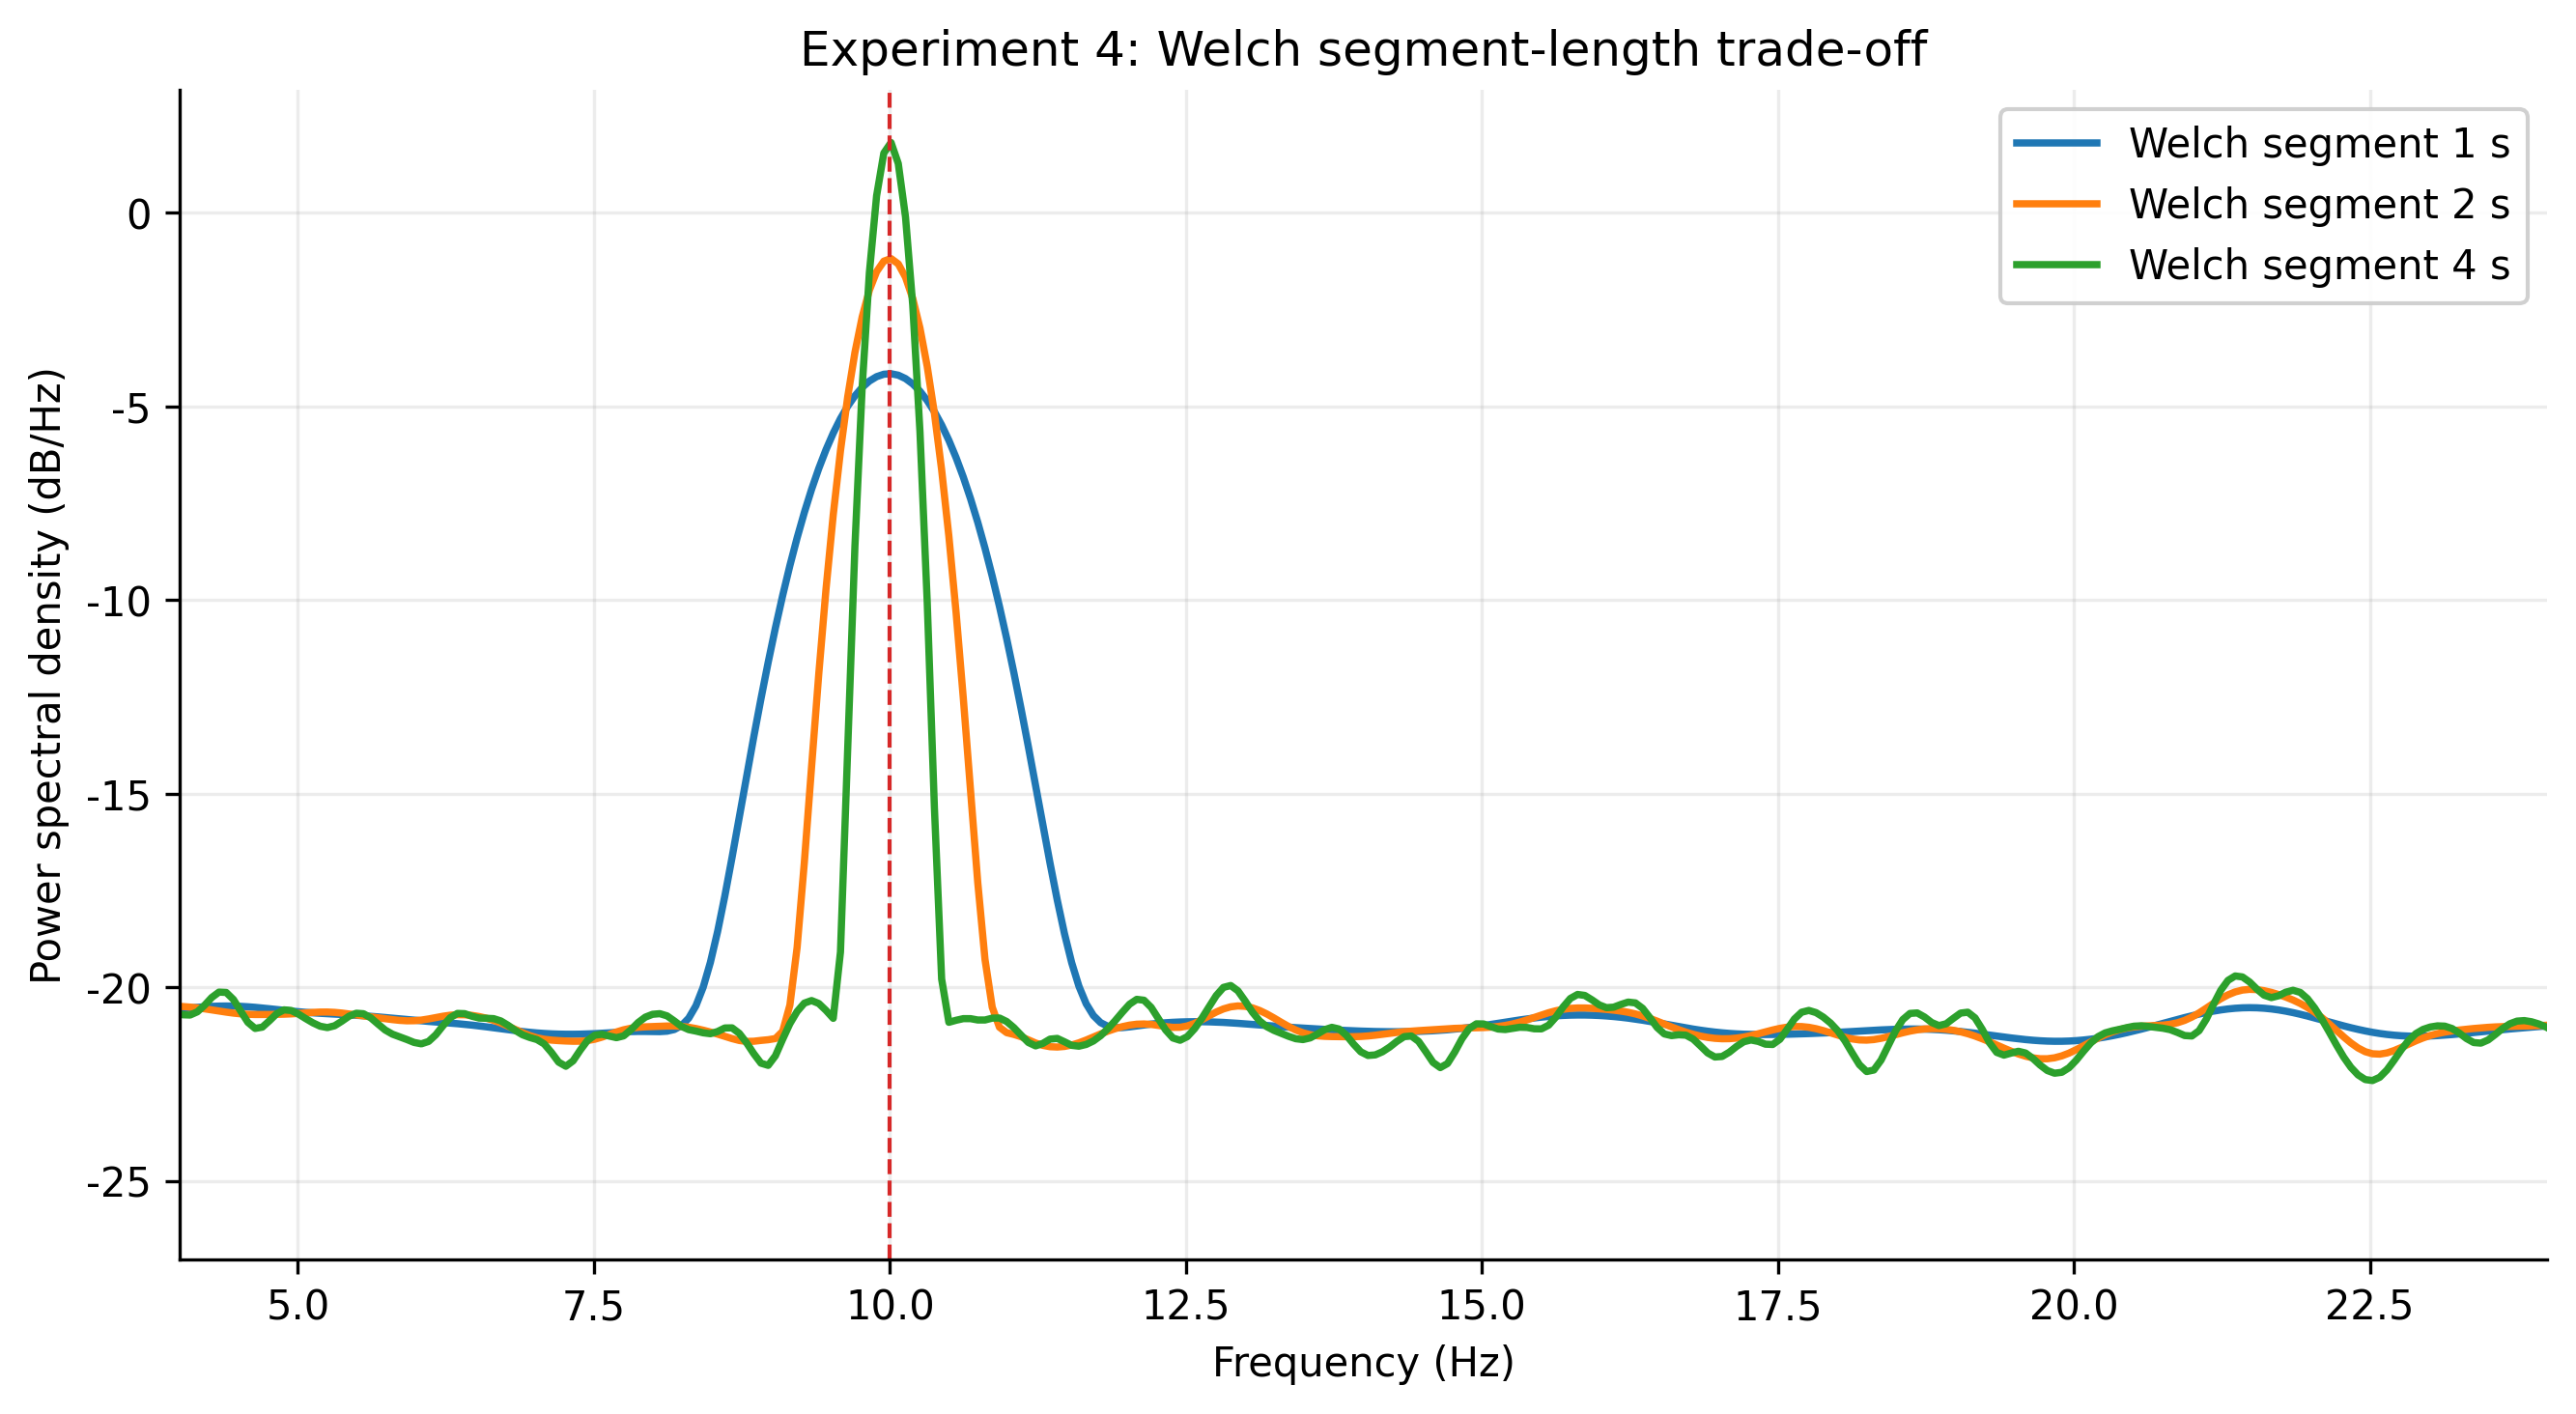
\includegraphics[width=\textwidth]{exp4_welch_segment_lengths_en.png}
\caption{Mean Welch spectra for different segment lengths.}
\end{figure}

\input{generated_en/table_exp4_segment.tex}

\subsection{Real EEG Windows}
The real Oz segment 58.84--112.84 s is split into nine non-overlapping 6 s windows. Each window is analyzed by a 6 s Hamming periodogram and by Welch with 2 s segments.

\begin{figure}[H]
\centering
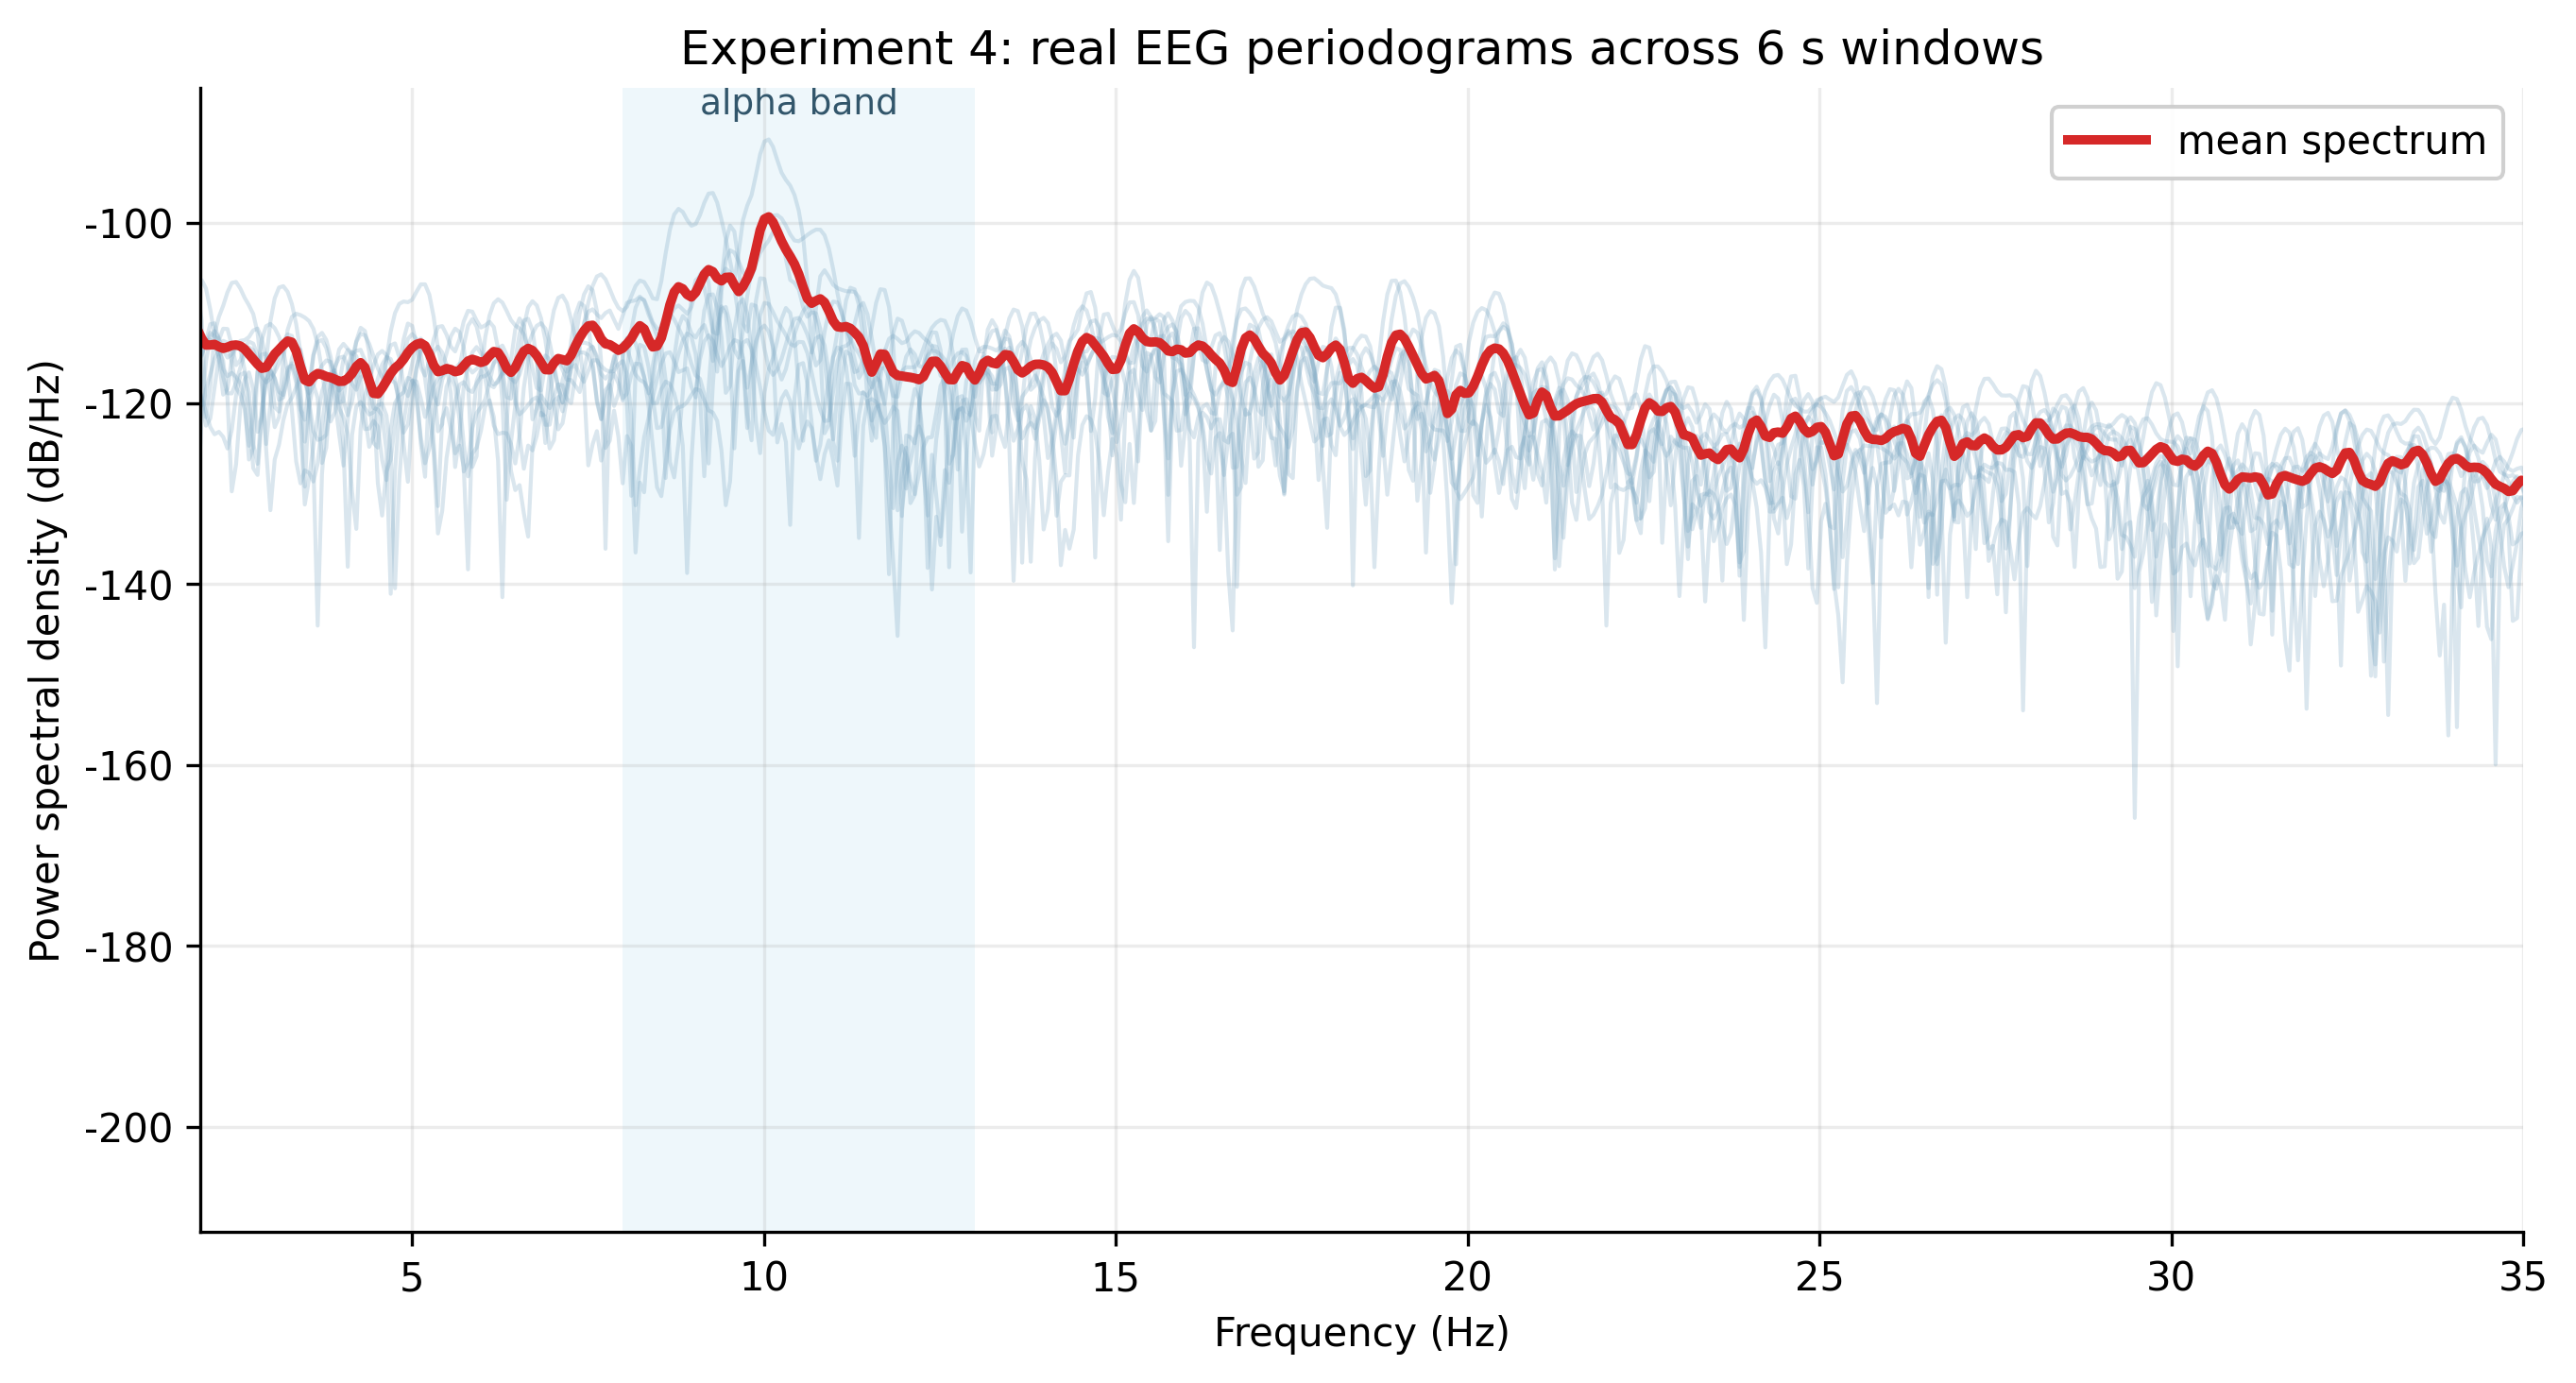
\includegraphics[width=\textwidth]{exp4_real_periodogram_windows_en.png}
\caption{Real EEG periodograms across nine 6 s windows.}
\end{figure}

\begin{figure}[H]
\centering
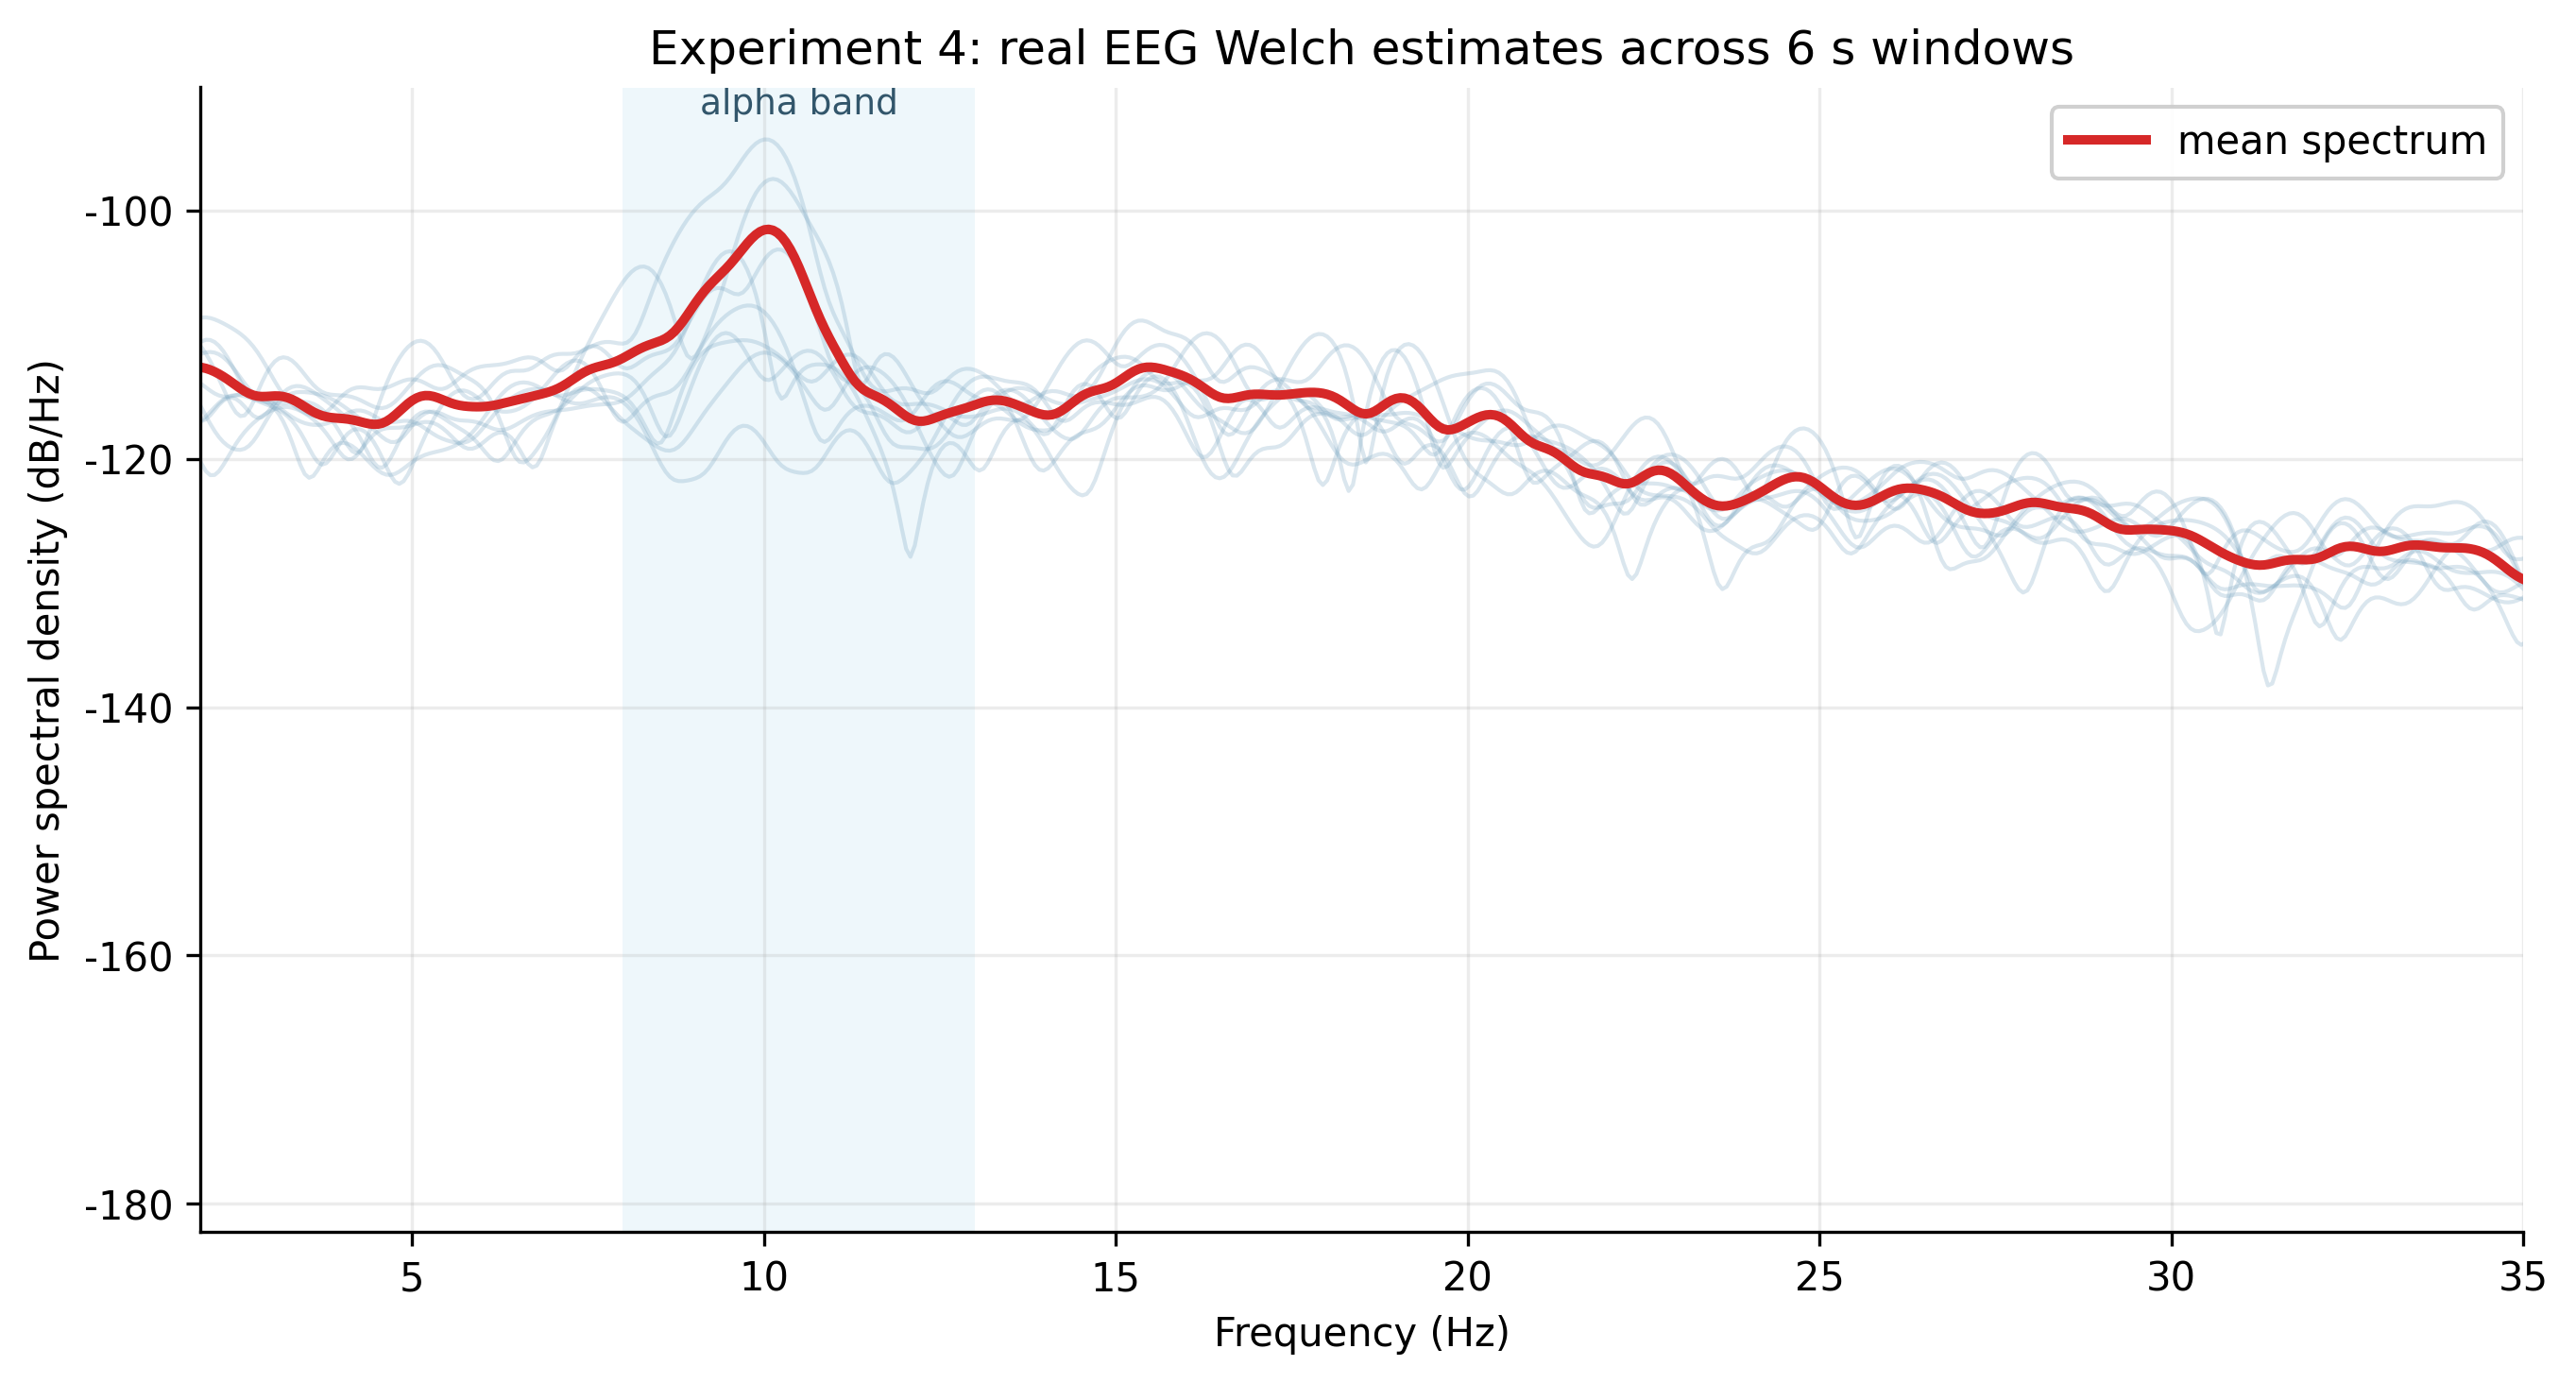
\includegraphics[width=\textwidth]{exp4_real_welch_windows_en.png}
\caption{Real EEG Welch spectra across nine 6 s windows.}
\end{figure}

\begin{figure}[H]
\centering
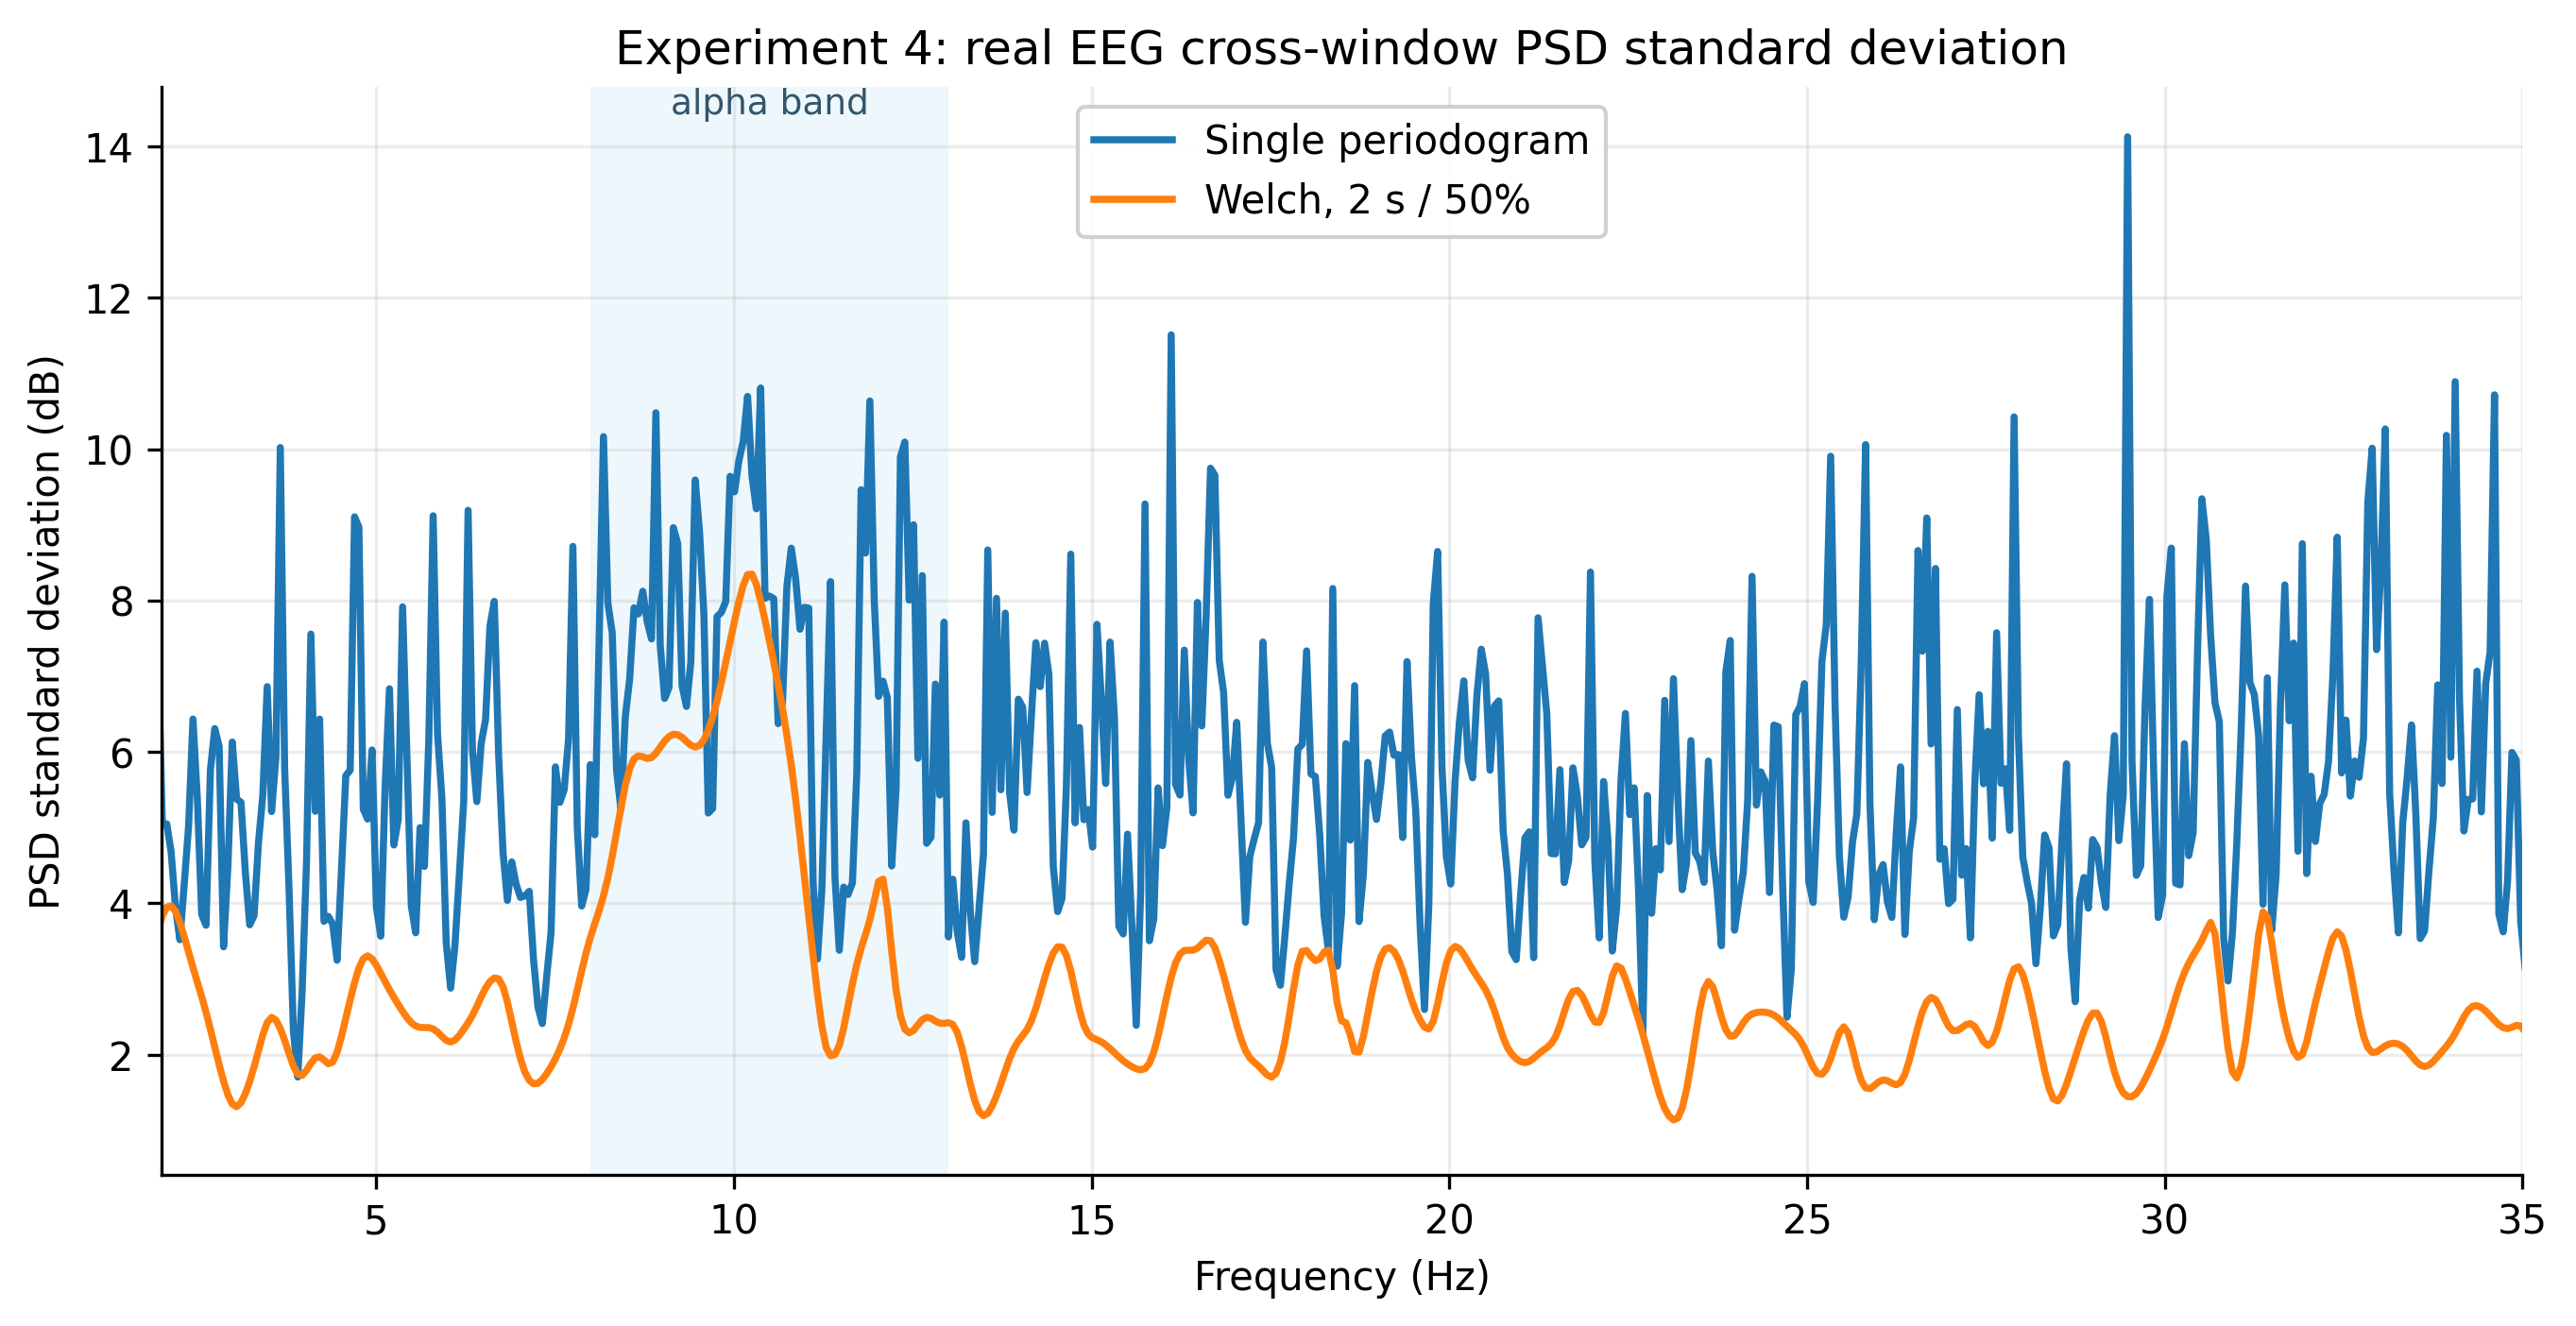
\includegraphics[width=\textwidth]{exp4_real_std_comparison_en.png}
\caption{Cross-window PSD standard deviation for the real EEG segment.}
\end{figure}

\input{generated_en/table_exp4_real.tex}

\subsection{Discussion}
Single periodograms fluctuate strongly across independent realizations even when the underlying random process is unchanged. Welch reduces estimator variance by averaging segment spectra. The cost is lower effective frequency resolution because each segment is shorter. In real EEG, Welch can reduce fine-scale estimator variance and jaggedness, but peak-frequency and prominence variability may still be dominated by nonstationary physiology rather than by the estimator alone.

\textbf{Question: What instability does Welch reduce?}
Answer: It reduces estimator variance across realizations or windows by averaging multiple segment periodograms. It does not eliminate true physiological variation across time.

\textbf{Question: Why is a more stable cross-window EEG spectrum not necessarily closer to the instantaneous neural state?}
Answer: Stability may come from temporal averaging. It can suppress meaningful short-lived neural changes while improving estimator smoothness.

\section{Overall Conclusions}

The four experiments support one central conclusion: a spectrum is not a neutral picture of the signal. It is an estimate shaped by record length, windowing, averaging, model order, and display choices. For synthetic signals, the ground-truth frequencies make the trade-offs explicit. For real closed-eye EEG, the same trade-offs directly affect alpha-band interpretation.

First, the direct FFT, periodogram, autocorrelation, and Welch estimates all detect the dominant spectral content, but their peak height, smoothness, bandwidth, and background floor differ. The full-lag biased autocorrelation implementation is intentionally close to the direct rectangular-window FFT, which is consistent with Wiener-Khinchin. This is defensible mathematically, but it also clarifies that a teacher or analyst may obtain a visibly different autocorrelation spectrum if the autocorrelation sequence is truncated or additionally windowed.

Second, physical frequency resolution is controlled by observation length. Larger NFFT values make the frequency grid denser and the plotted curve smoother, but they do not add information to the signal. Therefore a dense frequency axis must not be confused with a truly resolvable pair of close components.

Third, Welch averaging improves statistical stability by reducing estimator variance. This is clear in the cross-realization and cross-window standard-deviation plots. The price is a loss of effective frequency resolution when shorter segments are used. In real EEG, Welch reduces jagged estimator fluctuations, but true nonstationary physiological changes can still dominate alpha peak-frequency or prominence variability.

Fourth, AR spectra can look attractive because they generate sharp peaks from short data. However, AR sharpness depends strongly on model order. Low order can hide close peaks, while high order can split peaks or create pseudo-peaks. FPE is a useful prediction-error criterion, but it is not a guarantee of the most physiologically credible spectrum.

\section{Appendix A: Code Organization}

The implementation separates numerical computation, figure rendering, metric export, and report compilation so that the report can be edited without rerunning every experiment.

\begin{itemize}
  \item \texttt{src/spectral\_methods.py}: direct FFT, periodogram, autocorrelation, Welch, Yule-Walker AR, FPE, alpha metrics, valley-depth metrics, pointwise standard deviation, and peak-width utilities.
  \item \texttt{src/data\_io.py}: EEGLAB/MNE loading, direct \texttt{.fdt} fallback loading, volt-unit conversion, Oz channel lookup, and time-segment extraction.
  \item \texttt{src/plotting.py}: shared plotting style for the Chinese figures.
  \item \texttt{experiments/exp1.py}--\texttt{experiments/exp4.py}: experiment-specific computation, CSV metric export, cache writing, and Chinese figure generation.
  \item \texttt{experiments/run\_all.py}: full numerical reproduction pipeline for all four experiments.
  \item \texttt{experiments/run\_all\_en.py}: English figure rendering and the mechanism diagram used in this report and README.
  \item \texttt{report/report.tex}: Chinese report source.
  \item \texttt{report/report\_en.tex}: English report source.
  \item \texttt{report/build\_report.py}: Chinese table generation and PDF compilation.
  \item \texttt{report/build\_report\_en.py}: English table generation and PDF compilation.
  \item \texttt{outputs/tables/}: CSV metric tables used by both reports.
  \item \texttt{outputs/figures\_en/}: English figures used by GitHub and this English report.
\end{itemize}

\section{Appendix B: Core Code Snippets}

\subsection{Unified One-Sided PSD Scaling}
All FFT-based spectra use window-power normalization and one-sided energy doubling. This makes the PSD scale comparable across windows and methods.

\begin{lstlisting}[language=Python,caption={One-sided PSD scaling used by direct FFT and periodogram estimates.}]
def one_sided_from_fft(y, fs, nfft, scale_sum_sq):
    spec = np.fft.rfft(y, n=nfft)
    pxx = (np.abs(spec) ** 2) / (fs * scale_sum_sq)
    if nfft % 2 == 0:
        pxx[1:-1] *= 2.0
    else:
        pxx[1:] *= 2.0
    freqs = np.fft.rfftfreq(nfft, d=1.0 / fs)
    return freqs, pxx
\end{lstlisting}

\subsection{Welch Estimation}
Welch estimation is delegated to SciPy with explicit segment length, overlap, Hamming window, and density scaling.

\begin{lstlisting}[language=Python,caption={Welch PSD configuration.}]
freqs, pxx = signal.welch(
    demean(x),
    fs=fs,
    window="hamming",
    nperseg=int(round(segment_s * fs)),
    noverlap=int(round(segment_s * fs * overlap)),
    nfft=nfft,
    detrend=False,
    return_onesided=True,
    scaling="density",
)
\end{lstlisting}

\subsection{Yule-Walker AR and FPE}
AR coefficients are estimated with the Yule-Walker normal equations. FPE is then computed from the estimated driving-noise variance.

\begin{lstlisting}[language=Python,caption={Yule-Walker AR estimation and FPE.}]
r_full = signal.correlate(x, x, mode="full", method="fft") / n
r = r_full[n - 1 : n + order]
coeffs = solve_toeplitz((r[:order], r[:order]), -r[1 : order + 1])
noise_var = r[0] + np.dot(coeffs, r[1 : order + 1])
fpe = noise_var * (n + order + 1) / (n - order - 1)
\end{lstlisting}

\subsection{Alpha Metrics}
Alpha analysis uses a fixed 8--13 Hz peak band and a 15--30 Hz background band.

\begin{lstlisting}[language=Python,caption={Alpha peak, prominence, and width metrics.}]
peak_f, peak_db = band_peak(freqs, pxx_db, (8.0, 13.0))
background_db = band_mean_db(freqs, pxx_db, (15.0, 30.0))
alpha_prominence_db = peak_db - background_db
alpha_width_hz = minus_3db_width(freqs, pxx_db, (8.0, 13.0))
\end{lstlisting}

\subsection{EEG Unit Consistency}
The fallback EEGLAB reader converts microvolt-scale \texttt{.fdt} values to volts so that it matches MNE's \texttt{raw.get\_data()} convention.

\begin{lstlisting}[language=Python,caption={Fallback EEGLAB unit conversion.}]
raw = np.fromfile(fdt_path, dtype="<f4").reshape(n_channels, n_samples, order="F")
data_v = raw.astype(float) * 0.000001
return EEGData(X=data_v, fs=fs, ch_names=ch_names, unit="V", scale_factor=0.000001)
\end{lstlisting}

\section{Appendix C: Reproduction and Verification Commands}

\subsection{Environment Setup}
\begin{verbatim}
python -m venv .venv
.\.venv\Scripts\python.exe -m pip install --upgrade pip
.\.venv\Scripts\python.exe -m pip install -r requirements.txt
\end{verbatim}

\subsection{Full Reproduction}
\begin{verbatim}
.\.venv\Scripts\python.exe -m experiments.run_all
.\.venv\Scripts\python.exe -m experiments.run_all_en
.\.venv\Scripts\python.exe report\build_report_en.py
\end{verbatim}

\subsection{Chinese Report Build}
The Chinese report source is retained for reproducibility but the Chinese PDF is not published in the GitHub repository.

\begin{verbatim}
.\.venv\Scripts\python.exe report\build_report.py
\end{verbatim}

\subsection{Verification}
\begin{verbatim}
$files = @(Get-ChildItem src,experiments -Filter *.py |
  ForEach-Object { $_.FullName }) +
  @((Resolve-Path report\build_report.py).Path,
    (Resolve-Path report\build_report_en.py).Path)
.\.venv\Scripts\python.exe -m py_compile @files

pdftoppm -png -r 130 outputs\pdf\Spectral_Estimation_Lab_Report_EN.pdf ^
  tmp\pdfs\english_report_page
\end{verbatim}

Additional numerical checks used in development verified that all CSV tables contain no NaN/Inf numeric entries, that MNE and direct \texttt{.fdt} fallback loading give the same Oz-segment standard deviation after unit conversion, and that the English LaTeX log contains no missing-character, overfull-box, or fatal compilation errors.

\end{document}
